\documentclass[
%   crop, % erzeugt Schnittmarken auf A4
]{kspbook}
\setlength{\overfullrule}{5pt}
%\usepackage[utf8]{inputenc} % direct input of unicode chars like äöüß
%\usepackage[OT1]{fontenc}
\usepackage[ngerman, english]{babel}
\usepackage{blindtext}

%\usepackage[ansinew]{inputenc}
\usepackage[latin1]{inputenc}
%\usepackage[utf8]{inputenc}
\usepackage[T1]{fontenc}
\usepackage{mathptmx}

%
%\usepackage{ngerman}

\usepackage{graphicx}
\usepackage{booktabs}
\usepackage{multirow}
\usepackage{caption}
\usepackage{dcolumn}
%\usepackage{fancyhdr}
\usepackage{lscape}
\usepackage{rotating}
\usepackage{subfig}
\usepackage{amssymb}
\usepackage{stmaryrd}
\usepackage[mathscr]{euscript}
\usepackage{makeidx}
\usepackage{relsize}
\usepackage{microtype}
\usepackage{ziffer}
\usepackage{url}
\usepackage{tocbibind} 
\usepackage{float}
\usepackage{booktabs}
%\usepackage[style=altlist,toc=true,nonumberlist,acronym=true]{glossaries}
%\usepackage[inner=3cm,outer=4cm,top=3cm,bottom=3cm,includeheadfoot]{geometry}
%\usepackage{amsthm}
\usepackage[toc,page]{appendix}
\usepackage{listings}


\usepackage[bottom]{footmisc} % Fußnoten ans Ende der Seite
%\usepackage[ngerman]{babel}   % Silbentrennung nach der ndR, z.B.: Sys-tem
\usepackage{amstext}          % bietet Befehl \text{} für Text in Formeln
\usepackage{amsfonts}         % bietet Mengensymbole, $\mathbb{R}$
\usepackage{enumerate}        % verbessert Aufzählungen
\usepackage{array}            % für Tabellen: bindet tabular-Umgebung ein
\usepackage{algorithm}        % für List of Algorithms usw.
\usepackage{algorithmicx}      % für List of Algo usw., Vorsicht: neues .sty
\usepackage{ntheorem}
\usepackage{theorem}
%\usepackage{parskip}          % zw. Absätzen: eine knappe Leerzeile statt hängender Einzüge
\usepackage{indentfirst}      % rückt in der Bibl. auch ersten Absatz ein (aus)
\usepackage{xcolor}           % farbiger Text
\usepackage{multicol} 	      % zur Indexerstellung in zwei Spalten
\usepackage{url}              % für \url{http://www.test.com}
%\usepackage[numbers, square]{natbib}   % Für \setlength{\bibsep}{3mm}; square macht eckige Klammern
%\usepackage[isolatin]{inputenc} 
\usepackage{amsmath}
\usepackage{graphicx}
\usepackage{mathcomp}
\usepackage[sc]{mathpazo}
\usepackage{rotating}
\usepackage[noend]{algpseudocode}
\usepackage{pstool}
\usepackage{psfrag}
\usepackage{longtable}
\usepackage{tabu}
%\usepackage{subfloat}
%\usepackage{minipage}
\usepackage{hyperref}


%settings from beispiel

\newcolumntype{L}[1]{>{\raggedright\let\newline\\\arraybackslash\hspace{0pt}}m{#1}}
\newcolumntype{C}[1]{>{\centering\let\newline\\\arraybackslash\hspace{0pt}}m{#1}}
\newcolumntype{R}[1]{>{\raggedleft\let\newline\\\arraybackslash\hspace{0pt}}m{#1}}

%\usepackage[xindy]{glossaries}

%\linespread{1.05}         % Palatino needs more leading (space between lines)

\definecolor{KITBlue}{HTML}{4664aa}
\definecolor{KITGreen}{HTML}{009682}
\definecolor{KITRed}{rgb}{1.0,0.0,0.0}



%for quotations
\usepackage{epigraph} % mit \epigraphhead[5]{\epigraph{Zitat}{Autor}}
\setlength{\epigraphwidth}{.5\textwidth} % Breite des Zitats
\setlength{\beforeepigraphskip}{.5\baselineskip} % Abstand vor epigraph
\setlength{\afterepigraphskip}{.5\baselineskip} % Abstand nach epigraph
\setlength{\epigraphrule}{0pt} % keine Linie zw. Zitat und Autor

\DeclareFontFamily{OT1}{pzc}{}
\DeclareFontShape{OT1}{pzc}{m}{it}{<-> s * [1.10] pzcmi7t}{}
\DeclareMathAlphabet{\mathpzc}{OT1}{pzc}{m}{it}


\newtheorem{theorem}{Theorem}

\parindent 0pt
\setlength{\parskip}{0pt}
%\setlength{\parsep}{0pt}
\graphicspath{{./Bilder/}}

\newenvironment{packed_itemize}{
\begin{itemize}
  %\setlength{\itemsep}{0pt} % Definiert den Abstand, der zwischen zwei Listenpunkten (item) zusätzlich zum normalen parsep eingefügt wird.
  \setlength{\parskip}{0pt} % Legt den Abstand zwischen den nachfolgenden Absätzen fest.
  %\setlength{\parsep}{0pt} % Legt innerhalb einer Liste den Abstand zwischen zwei Absätzen fest.
  %\setlength{\topsep}{0pt} % Legt den Abstand fest, der vor und nach einer Liste zusätzlich eingefügt wird.
  %\setlength{\topmargin}{0pt}
}{\end{itemize}}


\sloppy                       % nicht so streng mit Umbrüchen


\renewcommand{\textfraction}{0.1}
\renewcommand{\topfraction}{0.85}
\renewcommand{\bottomfraction}{0.70}
\renewcommand{\floatpagefraction}{0.8}

%\renewcommand{\figurename}{Abb.}
%\renewcommand{\tablename}{Tab.}
\captionsetup{format=hang,justification=justified,labelfont=bf}


	
\renewcommand{\chaptermark}[1]{\markboth{\chaptername\ \thechapter.\ #1}{}} %
\renewcommand{\sectionmark}[1]{\markright{\thesection.\ #1}}
\addtolength{\headheight}{3.0pt}


%	\renewcommand{\headrulewidth}{0.3pt}




\makeindex                    % Befehl für die Indexerstellung	
                              % Obacht: stelle auch ein: TexnicCenter: Projekt / Eigenschaften
															
\setcounter{blindlistlevel}{2}%




\title{\LARGE{A short introduction to \\
soft tissue simulation}}
\author{Stefan Suwelack (ed.)\\
\\
{suwelack@kit.edu}
\vspace*{0.5cm}\\}
%\titlehead{Kopf}
%\subject{Typisierung}
%\subtitle{Untertitel}
%\date{Datum}
%\publishers{Herausgeber}
\lowertitleback{%
   
	Please help to make this book better by reporting errors or any other issue at \\
	\url{https://github.com/ssuwelack/soft-tissue-simulation/issues}.
	\vspace*{0.5cm}\\
	Are you a researcher? Please add a reference to your soft tissue simulation related work in the application chapter and submit a pull request.
	\vspace*{0.5cm}\\
	This is a joint work in progress. If you feel you have something to contribute to an introductory text for soft tissue simulation, please become an author of this book!
	\vspace*{0.5cm}\\
	
	
		
	Editor:	\\
	Stefan Suwelack, suwelack@kit.edu\\
	\vspace*{0.5cm}\\
	

    
\includegraphics[scale=1]{Figures/license.pdf}
 
	This work is licensed under a Creative Commons Attribution-ShareAlike $4.0$ Unported License: \\
	\url{http://creativecommons.org/licenses/by-sa/4.0/}.
	
	
}








%\selectlanguage{ngerman}

%elasticity basics
\newcommand{\mI}{\ensuremath{ \textnormal{I}}}

\newcommand{\mbu}{\ensuremath{\mathbf {u} }} 
\newcommand{\mbx}{\ensuremath{\mathbf {x} }} 
\newcommand{\mbX}{\ensuremath{\mathbf {X} }} 
\newcommand{\mbF}{\ensuremath{\mathbf {F }}} 
\newcommand{\mbdotF}{\ensuremath{\dot{\mbF} }} 
\newcommand{\mbdx}{\ensuremath{\textnormal{d} \mathbf {x }}} 
\newcommand{\mbdX}{\ensuremath{\textnormal{d} \mathbf {X }}} 
\newcommand{\mdx}{\ensuremath{\textnormal{d} {x }}} 
\newcommand{\mdX}{\ensuremath{\textnormal{d}  {X }}} 
\newcommand{\mbdu}{\ensuremath{\textnormal{d} \mathbf {u }}}
\newcommand{\mbI}{\ensuremath{ \mathbf {I }}}
\newcommand{\mdVZero}{\ensuremath{ \textnormal{dV}_0}}
\newcommand{\mdV}{\ensuremath{ \textnormal{dV}}}
\newcommand{\mdAZero}{\ensuremath{ \textnormal{dA}_0}}
\newcommand{\mdA}{\ensuremath{ \textnormal{dA}}}
\newcommand{\mbdAZero}{\ensuremath{ \textnormal{d}\mathbf{A}_0}}
\newcommand{\mbdA}{\ensuremath{ \textnormal{d}\mathbf{A}}}
\newcommand{\mdet}{\ensuremath{ \textnormal{det}}}
\newcommand{\mphi}{\ensuremath{\varphi}}
\newcommand{\msigma}{\ensuremath{\boldsymbol{\sigma}}}  
\newcommand{\mn}{\ensuremath{\mathbf {n} }} 
\newcommand{\mbN}{\ensuremath{\mathbf {N} }} 
\newcommand{\mbn}{\ensuremath{\mathbf {n} }} 
\newcommand{\mt}{\ensuremath{\mathbf {t} }} 
\newcommand{\mbg}{\ensuremath{\mathbf {g} }} 
\newcommand{\mbl}{\ensuremath{\mathbf {l} }} 
\newcommand{\mbd}{\ensuremath{\mathbf {d} }} 
\newcommand{\mbw}{\ensuremath{\mathbf {w} }} 

\newcommand{\mboF}{\ensuremath{\mathbf {\overline{F} }}} 
\newcommand{\mboC}{\ensuremath{\mathbf {\overline{C} }}}

\newcommand{\mrf}{\ensuremath{\mathcal G }} 
\newcommand{\mrF}{\ensuremath{\mathcal H }} 

\newcommand{\mbT}{\ensuremath{\mathbf {T} }} 
\newcommand{\mtr}{\ensuremath{\textnormal{tr} }} 
\newcommand{\mwint}{\ensuremath{w_{int}}} 

\newcommand{\mbV}{\ensuremath{\mathbf {V} }} 

\newcommand{\mgrad}{\ensuremath{ \textnormal{grad}}}
\newcommand{\mGrad}{\ensuremath{ \textnormal{Grad}}}
\newcommand{\mdiv}{\ensuremath{ \textnormal{div}}}
\newcommand{\mDiv}{\ensuremath{ \textnormal{Div}}}

\newcommand{\mddt}{\ensuremath{ \frac{\textnormal{D}}{\textnormal{Dt}}}}
\newcommand{\mddtS}{\ensuremath{ \frac{\textnormal{D}^2}{\textnormal{Dt}^2}}}
\newcommand{\mDDt}{\ensuremath{ \frac{\textnormal{D}}{\textnormal{Dt}}}}

\newcommand{\mbU}{\ensuremath{\mathbf {U} }} 
\newcommand{\mbC}{\ensuremath{\mathbf {C} }} 
\newcommand{\mbE}{\ensuremath{\mathbf {E} }} 
\newcommand{\mbeps}{\ensuremath{\boldsymbol \epsilon }}

\newcommand{\mPext}{\ensuremath{\mathcal P _{ext}}} 
\newcommand{\mPint}{\ensuremath{\mathcal P _{int}}} 
\newcommand{\mKext}{\ensuremath{\mathcal K }} 
\newcommand{\mK}{\ensuremath{\mathcal K }} 

\newcommand{\mcg}{\ensuremath{\mathcal{g}}} 
\newcommand{\mcG}{\ensuremath{\mathcal{G}}} 

\newcommand{\mcM}{\ensuremath{\mathcal{M}}} 

\newcommand{\mPsi}{\ensuremath{\Psi}} 


\newcommand{\mbdF}{\ensuremath{\textnormal{d} \mathbf {f} }} 


\newcommand{\mbP}{\ensuremath{\mathbf {P} }} 
\newcommand{\mbS}{\ensuremath{\mathbf {S} }} 

\newcommand{\mrho}{\ensuremath{\rho}}

\newcommand{\mBody}{\ensuremath{\mathcal{B} }} 
\newcommand{\mv}{\ensuremath{\mathbf {v} }} 
\newcommand{\mdotv}{\ensuremath{\mathbf {\dot v} }} 

\newcommand{\mdotu}{\ensuremath{\mathbf {\dot u} }} 

 
\newcommand{\mSt}{\ensuremath{\mathbf {U }}} 

\newcommand{\meFunc}{\ensuremath{\Pi}} 
\newcommand{\mH}{\ensuremath{H}} %Hamiltonian
\newcommand{\mL}{\ensuremath{L}} %Lagrangian
%\newcommand{\mPotEn}{\ensuremath{\Pi}} 

\newcommand{\meps}{\ensuremath{\boldsymbol{\epsilon}}} 

 
\newcommand{\mRConf}{\ensuremath{\Omega _0 }}  
\newcommand{\mCConf}{\ensuremath{\Omega }}
\newcommand{\mIntRConf}{\ensuremath{\int _{\Omega _0} }}
\newcommand{\mIntCConf}{\ensuremath{\int _{\Omega } }}
\newcommand{\mIntREl}{\ensuremath{\int _{\mElem} }}
\newcommand{\mIntBCRConf}{\ensuremath{\int _{\partial \Omega _0} }}
\newcommand{\mDRConf}{\ensuremath{\textnormal{dV}_0 }}
\newcommand{\mDCConf}{\ensuremath{\textnormal{dV} }}

\newcommand{\mcu}{\ensuremath{\mathcal{U} }} 
%\newcommand{\mca}{\ensuremath{\mathcal{A} }} 
\newcommand{\mcx}{\ensuremath{\mathcal{X} }} 
\newcommand{\mbf}{\ensuremath{N_J }} 
\newcommand{\mbffull}{\ensuremath{N_{jJ} }} 
\newcommand{\mtf}{\ensuremath{N_I }} 
\newcommand{\mtfTwo}{\ensuremath{N}} 
\newcommand{\mtfderiv}{\ensuremath{N_{I,i} }} 
\newcommand{\mtfn}{\ensuremath{N }} 

\newcommand{\mcdx}{\ensuremath{\textnormal{d}\mathpzc{x}  }}
\newcommand{\mcdv}{\ensuremath{\textnormal{d}\dot{\mathcal{U}}  }}
\newcommand{\mcdu}{\ensuremath{\textnormal{d}{\mathcal{U}}  }}

\newcommand{\mesym}{\ensuremath{T }} 
\newcommand{\mfsym}{\ensuremath{\partial T }} 

\newcommand{\mfext}{\ensuremath{\mathbf f ^{ext}}} 
\newcommand{\mfextTwo}{\ensuremath{\mathbf f ^{ext}_I}} 
\newcommand{\mfextThree}{\ensuremath{f  ^{ext}_{iI}}} 

\newcommand{\mfint}{\ensuremath{\mathbf f ^{int}}} 
\newcommand{\mfintTwo}{\ensuremath{\mathbf f ^{int}_I}} 
\newcommand{\mfintTwoX}{\ensuremath{\mathbf f ^{int}_I}} 
\newcommand{\mfintThree}{\ensuremath{f  ^{int}_{iI} }} 
\newcommand{\mfintDens}{\ensuremath{\hat{f}  ^{X,int}_{iI} }} 
\newcommand{\mfintDensTwo}{\ensuremath{\mathbf {\hat{f}} ^{int}_I}} 
\newcommand{\mfintDensTwoX}{\ensuremath{\mathbf {\hat{f}} ^{X,int}_I}} 

\newcommand{\mfintCR}{\ensuremath{\mathbf f ^{int,CR}}} 
\newcommand{\mfintTwoCR}{\ensuremath{\mathbf f ^{int,CR}_I}} 
\newcommand{\mfintThreeCR}{\ensuremath{f  ^{int,CR}_{iI} }}
\newcommand{\mfintDensCR}{\ensuremath{\hat{f}  ^{int,CR}_{iI} }}

\newcommand{\mnode}{\ensuremath{P}} 
\newcommand{\mnnode}{\ensuremath{n}} %number of all nodes
\newcommand{\mmnode}{\ensuremath{m}} %number of all extended nodes

\newcommand{\mmmat}{\ensuremath{\mathbf M}} 
\newcommand{\msmat}{\ensuremath{\mathbf K}}
\newcommand{\mdmat}{\ensuremath{\mathbf D}}

\newcommand{\mBCN}{\ensuremath{\Gamma _N}}
\newcommand{\mBCD}{\ensuremath{\Gamma _D}}
\newcommand{\mBCC}{\ensuremath{\Gamma _C}}

\newcommand{\mBCSPD}{\ensuremath{V_D(\mBCD,\overline{\mbu})}}
\newcommand{\mBCSPDX}{\ensuremath{V_D(\mBCD,\overline{\mbx})}}
\newcommand{\mBCSPN}{\ensuremath{V_N(\mBCN,\overline{\mt})}}
\newcommand{\mBCSPC}{\ensuremath{V_C(\mBCC,0)}}


\newcommand{\mTFunc}{\ensuremath{\delta \mbu}}  
\newcommand{\mSTFunc}{\ensuremath{{C}_0 ^{\infty}}}
\newcommand{\mSCTFunc}{\ensuremath{{C}_0 ^{\infty} \cap V_D(\mBCD,0)}}
\newcommand{\mSCTFuncTwo}{\ensuremath{{C}_0 ^{0} \cap V_D(\mBCD,0)}}
\newcommand{\mSCTFuncThree}{\ensuremath{{H}^1  \cap V_D(\mBCD,0)}}

\newcommand{\mSSol}{\ensuremath{{C} ^{2}(\Omega) \cap {C} ^{1} (\overline{\Omega})}}
\newcommand{\mSSolBC}{\ensuremath{{C} ^{2}(\Omega) \cap {C} ^{1} (\overline{\Omega}) \cap \mBCSPD \cap \mBCSPN}}

\newcommand{\mca}{\ensuremath{{\mathcal{\ddot{U}}}}}
\newcommand{\mcv}{\ensuremath{{\mathcal{\dot{U}}}}}

\newcommand{\mtvh}{\ensuremath{\hspace*{0.2em}^{t+\Delta t}\vspace*{-0.2em} }}
\newcommand{\mth}{\ensuremath{\hspace*{0.2em}^{t}\vspace*{-0.2em} }}
\newcommand{\mthZero}{\ensuremath{\hspace*{0.2em}^{0}\vspace*{-0.2em} }}

\newcommand{\mdt}{\ensuremath{\Delta t }}

\newcommand{\mintdt}{\textnormal{dt}}

\newcommand{\mrot}{\ensuremath{\mathbf{R}}}

\newcommand{\mstretchmat}{\ensuremath{\mathbf{U}}}

\newcommand{\mMesh}{\mathcal{M}}
\newcommand{\mSMesh}{\mathcal{S}}
\newcommand{\mElem}{\tau}
\newcommand{\mTri}{\mathbb{T}}
\newcommand{\mVert}{\nu}
\newcommand{\mbp}{\mathbf{p}}

\newcommand{\mElemSetVert}{\mathcal{E}}
\newcommand{\mVertSetElem}{\mathcal{V}}

\newcommand{\oProd}{\otimes}
\newcommand{\liftOp}{\mathbf O}









%\makeglossaries

% customize chapter format:
\KOMAoption{headings}{twolinechapter}
\renewcommand*\chapterformat{\thechapter\autodot}

% customize dictum format:
\setkomafont{dictumtext}{\itshape\small}
\setkomafont{dictumauthor}{\normalfont}
\renewcommand*\dictumwidth{\linewidth}
\renewcommand*\dictumauthorformat[1]{--- #1}
\renewcommand*\dictumrule{}


                         %   Use current date. 

% Note that book class by default is formatted to be printed back-to-back.
\begin{document}                        % End of preamble, start of text.
\frontmatter                            % only in book class (roman page #s)
\maketitle                              % Print title page.
\tableofcontents                        % Print table of contents

\pagestyle{scrheadings}

\mainmatter

\part{Theory}  

\setchapterpreamble[or][.5\textwidth]{%
\dictum[Edwin Schlossberg]{%
The skill of writing is to create a context in which other people can think.}\vskip1em}

%\setchapterpreamble[o]{%
%\dictum[Edwin Schlossberg]{The skill of writing is to create a context in which other people can think.}}

\chapter{Introduction}
%\epigraphhead[5]{\epigraph{The skill of writing is to create a context in which other people can think.}{Edwin Schlossberg}}
%\epigraphhead[5]{\epigraph{The skill of writing is to create a context in which other people can think.}{Edwin Schlossberg}}
%\thispagestyle{empty}
Modeling soft tissue by means of continuum mechanics has become an active area of research in many fields such as patient-specific surgery simulation, non-rigid image registration and cardiovascular diagnostics. However, it currently is a very young discipline that evolves at a rapid pace (and has arguably to mature much more before these methods become part of the daily clinical routine). When I was looking for literature that could be recommended to my students I felt that there is currently no real introductory textbook on this matter. This little script is to serve exactly this purpose. Although it is in most parts a short course on elasticity theory and the finite element method (FEM), it should also hint to recent research results in terms of material laws, special FEM algorithms and applications of soft tissue simulation.

The intended audience of this text are postgraduate level students with a computer science or engineering background. Its purpose is to introduce the most important ideas, principles and methods in the area of soft tissue simulation and it should serve as an introductory text either for self study or accompanying a lecture. It was in particular written with two specific goals in mind. On the one hand you should be able to implement your own simple soft tissue simulation using a linear FEM algorithm once you've completed this course. On the other hand the script should give you a general idea on the topic and should serve as a good starting point for further studies. 

For the impatient, here is a list of the topics currently covered by this text:

\begin{itemize}

		\item Introduction to elasticity: Strain, stress, balance principles and mechanical energy
		\item Material laws: Work conjugacy, linear elasticity, hyperelasticity, viscoelasticity
		\item The road to discretization: Variational formulation and weak form
		\item The finite element method: Shape functions, matrix formulation, numerical integration
		\item Time integration and projective constraint handling
		\item Efficient real-time models: Corotated tetrahedra
		\item Linear solvers: Conjugate gradients, preconditioners and multigrid
			
\end{itemize}

There are many great text books and internet resources about elasticity and the FE method. For further reading and in order to complement this text I recommend the following ones which I found exceptionally useful:

\begin{itemize}

		\item The textbook \emph{Nonlinear solid mechanics} by Gerhard Holzapfel provides thorough, yet concrete treatment of non-linear elasticity. It's a great read especially for engineers. The notation used in this text closely follows the notation by Holzapfel, so his book would make the perfect follow up to this script if you would like to really understand elasticity theory.
			\item If you prefer a highly mathematical treatment of the subject then the book \emph{Mathematical foundations of elasticity} by Jerrold Marsden and Thomas Hughes is definitely worth a look.
			\item In my opinion the book \emph{Nonlinear Finite Elements for Continua and Structures} by Belitschko et al. provides an excellent introduction to the finite element method and strikes a good balance between mathematical rigor and practical examples.
			\item If you would like to take a deeper look at error estimation methods as well as linear solver technology the book \emph{Finite Elements: Theory, Fast Solvers, and Applications in Solid Mechanics} by Dietrich Braess is a useful read.
			\item For a more general introduction into numerics I highly recommend the book \emph{Numerical Analysis} by Endre S\"uli and David MAyers
			\item In my opinion you cannot completely understand numerical methods without actually running them. That's why I highly recommend \url{www.solidmechanics.org} run by A.F. Bower where you can find lots of MATLAB sample code. 			
			
\end{itemize}

Although a detailed treatment of recent research results and applications in the context of soft tissue simulation is out of scope for this document, such work is referenced in the application chapter. If you know of any work that should be listed there, please submit a pull request or write me an e-mail.

I have always been fascinated how simulations turn equations and numbers into something that mimics reality. I am therefore convinced that learning about simulation methods must include seeing this process in action. In order to make this possible, this document contains a tutorial section which contains hands-on examples and exercises based on state-of-the-art open source simulation tools.

This book is distributed under a CC-BY-SA license. My biggest wish is that it will be copied, edited, corrected and enhanced by anyone who finds it a good seedpoint for his/her own work. If you feel there is something missing (which there definitely is), please become an author of this book! 

Finally I'd be delighted to hear from you if you found this text useful for your studies, thesis work or research. You can reach me by e-mail under suwelack(at)kit.edu. \\
\\
Karlsruhe, Germany, 2015\\
\\
Stefan Suwelack





\setchapterpreamble[or][.5\textwidth]{%
\dictum[John von Neumann]{%
If people do not believe that mathematics is simple, it is only because they do not realize how complicated life is.}\vskip1em}

\chapter{Biomechanical modeling of soft tissue}
%\epigraphhead[5]{\epigraph{ If people do not believe that mathematics is simple, it is only because they do not realize how complicated life is.}{ John von Neumann}}

In this chapter the foundations of continuum mechanics based soft tissue modeling are introduced. We start by outlining the fundamentals of elasticity theory before presenting typical material models for biological soft tissue. 

\section{Getting started}

Mechanics is often defined as \emph{... a branch of physics concerned with the behaviour of physical bodies when subjected to forces or displacements, and the subsequent effect of the bodies on their environment}. You will most certainly remember some experiments from your physics class in school where you tried to calculate the paths of colliding billiard balls by using physical principles such as the energy and impulse conservation laws. If you have some background in thermodynamics you might be familiar with systems that consist of huge numbers of particles (statistical mechanics). If you had to deal with semiconductors during your studies you certainly have encountered the strange behavior of particles at the atomic and subatomic scales (quantum mechanics). Now, what is meant by the term \emph{continuum mechanics} and why is this set of methods useful for soft tissue simulation?

Imagine you would like to design a computer-based training tool that allows a surgeon to practise the removal of a liver tumor (partial liver resection) before actually performing the surgery on a patient. During surgery the liver is not only subject to the forces created by surgical instruments, but also to the forces originating from breathing motions. In order to simulate the deformations (i.e. the displacement of all points inside the liver) that occur from these forces we first have to think of a suitable computer model. Keep in mind that we always want to solve the problem as fast as possible (in this case even in real-time). Thus, the model has to be as accurate as required, but as simple as possible. We would be very ill-advised to try to model the behaviour of each atom in the liver by quantum mechanics. Even the modeling of every cell in the liver would require computing power that is far beyond the capability of current hardware. To effectively model the mechanical behavior of the liver we have to turn to a macroscopic model. In this sense a liver consists of different materials such as healthy liver tissue, blood vessels or tumor tissue. We now assign these materials to the corresponding sections of the liver. Within each section the liver is assumed to be continuous. If we chop down a piece of the liver until we have an infinitesimal small element we will therefor not find any cells, molecules or atoms, but instead just an infinitesimal element of the selected material. We will later see that the analysis of infinitesimal elements is in fact what continuum mechanics is all about. 


\section{A short introduction to elasticity}
\subsection{Kinematics}
We consider a body $\mBody$ that can be viewed as a continuous distribution of matter in space and choose a standard right-handed orthonormal coordinate system as the reference frame (Fig. \ref{BodyDeformation}). The body moves in space from one instant of time to another, occupying different geometrical regions $\Omega_0, ..., \Omega$ in the process. These regions are called configurations of $\mBody$ at time t. The configuration $\Omega_0$ at time $t=0$ is called the initial configuration while the configuration $\Omega$ at t is called the current configuration. Our goal is to describe the deformation of $\mBody$ with respect to a reference configuration. Throughout this text, we will always assume the initial configuration to be our reference configuration. 

\begin{figure}
   \centering   
   \psfragfig[width=0.9\textwidth]{Figures/ContinuumBodyDeformation}
	\caption{Deformation of the body $\mBody$ with material points $P,Q$ and infinitesimal line element $\mbdX$ from the reference configuration $\Omega_0$ to the current configuration $\Omega$ (based on \cite{Wikipedi2013})}
\label{BodyDeformation}
\end{figure}

We start by analyzing a continuum particle $\mathbf P \in \mBody$. It is important to note that $\mathbf  P$ has no point mass (as opposed to a discrete particle in Newtonian mechanics). The particle is at position $\mbX$ in the reference configuration and moves to the position $\mbx$ in the current configuration (Fig. \ref{BodyDeformation}). We define the vector field 
\begin{equation}
\mbx = \mphi (\mbX,t)
\end{equation}
that maps the positions $\mbX \in \mathcal{B}$ of all points in the reference configuration to their respective positions $\mbx$ in the current configuration. In our analysis we assume that $\mphi$ possess a continuous derivative and that it is uniquely invertible, i.e. the inverse mapping
\begin{equation}
\mbX = \mphi^{-1} (\mbx,t)
\end{equation}
exists. Here, some important terminology should be introduced. $\mphi$ is also called the motion of the body $\mBody$ over time. If we look at $\mphi$ at a specific point in time, $\mphi$ is called the deformation of the body. Thus, we speak of deformation if we mean the motion of a body that is independent of time. A body undergoing a deformation can change its shape, position and orientation. If the deformation is constant for all $\mbX \in \mBody$, the deformation consists only of translations and rotations and is called a rigid-body motion. Please note that in contrast to the common definition of deformation which implies changes to the body's shape, the continuum mechanics definition also includes rigid body motions.

Often the deformation is described in terms of the displacement
\begin{equation}
\mbu(\mbX,t)=\mbx(\mbX,t)-\mbX
\label{DisplacementDefinition}
\end{equation}
of the body $\mBody$. 

Continuum mechanics can be regarded as describing the behavior of infinitesimal line, area and volume elements during the passage from the reference to the current configuration. The second order tensor  
\begin{equation}
\mbF(\mbX,t) = \frac{\mbdx}{\mbdX} = \frac{\mdx_i}{\mdX_j}  = x_{i,j} = \nabla \mbx = \mGrad \mbx
\label{DeformationGradient}
\end{equation}
describes the relation between the spatial line element $\mbdx$ and the material line element $\mbdX$ and is called the deformation gradient. Here, we showcased several different notations for the deformation gradient: The vectorial notation, the index notation and its shortened version as well as the notation using the nabla and the material gradient ($\mGrad$) operator. For more information on the notation of variables and operators used in this thesis please refer to the glossary. Using the relation (\ref{DisplacementDefinition}), the deformation gradient can also be expressed in terms of the displacement field $\mbu (\mbx, t)$:

\begin{equation}
\mbF(\mbX,t) = \frac{\mbdu}{\mbdX} + \mbI = u_{i,j} + \delta _{ij} = \nabla \mbu + \mbI = \mGrad \mbu + \mbI 
\label{DeformationGradientDisplacement}
\end{equation}

Assuming that the derivative of the inverse mapping $\mphi^{-1}$ exist, we can define the inverse of the deformation gradient 
\begin{equation}
\mbF^{-1} = \frac{\mbdX}{\mbdx} = \mgrad \mbX
\label{InverseDeformationGradient}
\end{equation}
in an analogous manner. Please notice that the lowercase $\mgrad$ operator denotes the derivative with respect to $\mbx$ (spatial gradient).

\subsection{Deformation of infinitesimal elements}
\label{DeformationOfInfinitesimalElements}

In order to describe the change of infinitesimal volume elements due to deformation, we regard the parallelepiped that is spanned by the three non-coplanar line elements $\mbdX ^{(1)},\mbdX ^{(2)},\mbdX ^{(3)}$ at the point $\mbX$ in $\mBody$. Assuming that this triad is positively oriented, its volume $\mdVZero$ in the reference configuration 
 \begin{equation}
\mdVZero = (\mbdX^{(1)} \times \mbdX^{(2)}) \cdot \mbdX^{(3)} = \mdet (\mbdX ^{(1)},\mbdX^{(2)},\mbdX^{(3)} )
\label{Parallelepiped}
\end{equation}
is given by the triple scalar product. In accordance with eq. (\ref{DeformationGradient}) we can write
 \begin{equation}
\mbdx^{(i)} = \mbF \mbdX^{(i)}
\end{equation}
and can thus derive the volume 
 \begin{equation}
\mdV = (\mbdx^{(1)} \times \mbdx^{(2)}) \cdot \mbdx^{(3)} = \mdet ( \mbF \mbdX ^{(1)}, \mbF \mbdX ^{(2)}, \mbF \mbdX ^{(3)} )
\label{DeformedParallelepiped}
\end{equation}
of the deformed element. Using the relationship 
\begin{equation}
\mdet(\mathbf A \mathbf B) = \mdet(\mathbf A ) \mdet( \mathbf B)
\end{equation}
we can finally derive
 \begin{equation}
\mdV =  \mdet ( \mbF ) \mdet ( \mbdX ^{(1)},  \mbdX ^{(2)},  \mbdX ^{(3)} ) = \mdet ( \mbF ) \mdVZero \equiv J \mdVZero.
\end{equation}
The determinant $J$ of the deformation tensor (i.e. the Jacobian of the transformation $\mphi$) is the local ratio of current volume to reference volume of a material volume element. By definition (impenetrability of matter and non-singularity of $\mbF$), 
 \begin{equation}
J \equiv \mdet \mbF > 0.
\end{equation}

It is also important to point out, especially in the context of soft tissue modeling, that for incompressible materials $J = 1$.

We now seek to describe the deformation of the infinitesimal surface element $\mdAZero$ with the normal $\mbN$ from its reference configuration $\mbdAZero= \mdAZero \mbN$ to its current configuration $\mbdA= \mdA \mn$. We start by expressing the volume of a deformed parallelepiped eq. (\ref{DeformedParallelepiped}) 
 \begin{equation}
\mdV = \mbdA \cdot \mbdx = J \mdVZero = J \mbdAZero \cdot \mbdX
\end{equation}

through its base area. Noting that
 \begin{equation}
 \mbdA \cdot \mbdx = \mbdA \cdot \mbF \mbdX = \mbF ^T \mbdA \cdot \mbdX,
\end{equation}

we can derive 
 \begin{equation}
\underbrace{(\mbF ^T \mbdA - J  \mbdAZero) }_{0} \cdot \mbdX= 0
\end{equation}

As this must hold for arbitrary line elements $\mbdX$, we can describe the deformation of the arbitrary surface element $\mbdAZero$ through the deformation gradient tensor $\mbF$:
 \begin{equation}
\mbdA = J \mbF^{-T} \mbdAZero
\label{NansonsFormula}
\end{equation}
This relationship is known as Nanson's formula.

\subsection{Strain measures}
\label{SectionPolarDecomposition}

The deformation gradient tensor characterizes the deformation of infinitesimal line, area and volume elements during the body motion. In order to construct meaningful material laws it is necessary to determine the strain (i.e. the 3D equivalent of stretch) inside a body. Strain can be described as a measure for the change in length of infinitesimal line elements. It should be pointed out that strain is not a necessarily a physically measurable quantity, but rather a theoretical concept. Consequently, many different strain measures exist. In the following, the most important strain tensors for soft tissue modeling are presented.

First, it is important to understand that the deformation gradient tensor is not a suitable strain tensor; this can be seen from the polar decomposition theorem.

\begin{theorem}
The polar decomposition theorem: For any non-singular second order tensor $\mathbf A$ there exist a unique symmetric, positive definite second order tensor $\mbU$ and an orthogonal second-order tensor $\mrot$ such that
\begin{equation}
\mathbf A = \mrot \mbU
\end{equation}
\label{PolarDecompTheorem}
\end{theorem}

For a proof we refer to Ogden \cite{Ogden1997}. With respect to the deformation gradient tensor (keep in mind that it is non-singular) this means that it can be decomposed into a pure rotation matrix $\mrot$ and a pure stretch matrix $\mbU$. Thus, $\mbF$ changes under pure rigid body motions. For apparent reasons, the invariance under rigid body motions is an important property of a useful strain measure. Thus $\mbF$ cannot be directly used as a strain tensor. One possibility to recover rotational invariance is to perform a polar decomposition for each computation step and to use the remaining stretch matrix as a strain measure. Alternatively, a quadratic strain measure can be used. The first approach is often used in real-time simulations (see chapter \ref{RealTimeFEMChapter}), while the second possibility is used in classical solid mechanics as it allows for a better analytic analysis of the ensuing equations. 

Upon inserting the deformation gradient tensor into the Cauchy-Green strain tensor 
 \begin{equation}
\mbC = \mbF ^T \mbF
\label{CauchyGreenTensor}
\end{equation}

it is easy to see that $\mbC$ is rotation invariant (keep in mind that $\mrot^T \mrot = \mathbf I$ due to the orthogonality of $\mrot$):
 \begin{equation}
\mbC = \mbF ^T \mbF = (\mrot \mbU)^T \mrot \mbU =  \mbU ^T \mrot ^T \mrot \mbU = \mbU ^T  \mbU.
\end{equation}

Another important strain measure is the related Green-Lagrange strain tensor
 \begin{equation}
\mbE = \frac{1}{2} ( \mbC - \mbI ) =  \frac{1}{2} ( \mbF ^T \mbF - \mbI )  = \frac{1}{2} ( (\nabla \mbu + \mbI )^T (\nabla \mbu + \mbI ) - \mbI ),
\label{GreenLagrangeTensor}
\end{equation}
which is also symmetric and rotation invariant. Please note that both tensors are non-linear and must be in order to be rotation invariant. In order to facilitate the development of linear elasticity theory later on, we list the infinitesimal strain tensor 
 \begin{equation}
\mbeps =  \frac{1}{2} ( \nabla \mbu +  \nabla \mbu ^T ),
\label{InfinitesimalStrainTensor}
\end{equation}
which is the linearization of the Green-Lagrange strain tensor.

\subsection{Balance principles}
In classical continuum mechanics, the behavior of objects is governed by four conservation laws: The conservation of mass, the balance of linear and angular momentum as well as the conservation of energy. 

It is intuitively clear, that the body $\mBody$ is a closed system and its mass $m$ does not change, even if $\mBody$ does occupy different geometrical regions $\Omega_0, ..., \Omega$ over time. If we denote the density of $\mBody$ with $\rho _0(\mbX)$ in the reference configuration and the density in the current configuration with $\rho (\mbx)$ we thus require the mass to be the same in the current and in the reference configuration:
 \begin{equation}
m = \int _{\Omega_0} \rho _0(\mbX) \mdVZero = \int _{\Omega} \rho (\mbx) \mdV = \textnormal{const.}>0
\label{MassConservation}
\end{equation}
This is the conservation of mass in integral form. The linear momentum in the current configuration
 \begin{equation}
\int _{\Omega} \rho \mv \mdV = \int _{\Omega} \rho \dot \mbx \mdV
\label{LinearMomentum}
\end{equation}

is changed, when $\mBody$ is subjected to external forces. In this context, so called volumetric body forces (e.g. gravity, electromagnetic forces) are distinguished from contact forces that act on the surface of $\mBody$. The gravitational body force 
 \begin{equation}
\int _{\Omega} \rho \mbg \mdV 
\label{GravitationalForce}
\end{equation}
 can be written in its integral form using the gravitational constant $\mbg$. An analogous integral description for the contact force
 \begin{equation}
\int_{\partial \Omega}  \mt ( \mbx, \partial \Omega) \mbdA
\label{ContactForce}
\end{equation}
can be found by defining the contact force density (or surface traction vector) $\mathbf{t} (\mathbf x, \partial \Omega)$. The balance of linear momentum can be written as
 \begin{equation}
\int_{\partial \Omega}  \mt (\mbx, \partial \Omega) \mbdA + \int_{\Omega}   \rho \mbg \mdV  \equiv \mddt \int _{\Omega} \rho \mv \mdV  = \int _{\Omega} \rho \mdotv \mdV. 
\label{BalanceLinearMomentum}
\end{equation}
 For a body to be in complete equilibrium it is not sufficient that all internal and external forces acting on the body are in balance. Even if all external forces cancel out (static equilibrium) the body can still be subjected to a rotational motion, if these forces act on different points of the body. The rotational equilibrium is ensured by the balance of rotational momentum. By using the position vector $\mathbf r (\mbx) = \mbx - \mbx _0$ relative to a fixed point $\mbx_0$ it can be formulated as
 \begin{equation}
\int_{\partial \Omega}  \mathbf r \times \mathbf{t} (\mathbf x, \partial \Omega) \mbdA + \int_{\Omega}   \mathbf r \times  \rho \mbg \mdV  \equiv \mddt \int _{\Omega}  \mathbf r \times  \rho \mathbf v \mdV  = \int _{\Omega}  \mathbf r \times  \rho \mathbf{  \dot{v}} \mdV.
\label{BalanceRotationalMomentum}
\end{equation}




In the context of thermodynamics the conservation of energy and the balance of momentum is supplemented by the conservation of energy. However, in the realm of soft tissue simulation the thermal effects of the body motion are extremely small and are usually neglected. Thus, the body motion can be fully described using the three balance principles described above.



\subsection{The concept of stress}
Cauchy postulated that the surface traction vector $\mathbf t$ has the same value for all boundaries with the same normal direction $\mathbf n$. In other words, $\mathbf t$ only depends on the surface normal and we can write:
 \begin{equation}
\mt (\mbx, \partial \Omega) = \mt (\mbx, \mn).
\end{equation}
From this postulate, Cauchy's fundamental stress theorem can be established.
\begin{theorem}
Cauchy's stress theorem: Provided that it is continuous in $\mbx$, the stress vector $\mt(\mbx, \mn)$ depends linearly on $\mn$, i.e. there exists a second order tensor field $\msigma$ independent of $\mn$, such that
\begin{equation}
\mt (\mbx, \mn) = \sigma (\mbx)  \mn
\label{CauchyTheoremEquation}
\end{equation}
for all $\mbx$ in $\mBody$. The tensor $\msigma$ is called the Cauchy stress (or true stress) tensor.
\end{theorem}

\begin{figure}
   \centering   
   \psfragfig[width=0.6\textwidth]{Figures/CauchyTetrahedron}
	\caption{Cauchy's tetrahedron: The traction $\mt^{(\mn)}$ on the surface with normal $\mn$ can be expressed as a linear combination of the tractions on the coordinate planes (based on \cite{Wikipedi2013}).}
\label{CauchyTetrahedron}
\end{figure}

The theorem is usually proven (\cite{Ogden1997}, \cite{Bonet1997}) by constructing a tetrahedron that lies in the Cartesian rectangular planes (see Fig. \ref{CauchyTetrahedron}). After applying the balance of linear momentum eq. (\ref{BalanceLinearMomentum}) and collapsing the height of the triangle ($h \mapsto 0$) the external body and inertia forces vanish. The application of the postulate then leads to Cauchy's stress tensor. Furthermore, it can be shown that the balance of rotational momentum implies the symmetry of the Cauchy stress tensor \cite{Holzapfel2001}.

As a direct consequence we can express the force
\begin{equation}
\mbdF =  \mt (\msigma , \mn ) \mbdA = \msigma (\mbx) \mn \mdA
\label{SurfaceTractions}
\end{equation}
on an infinitesimal surface element (the so called surface tractions) in the current configuration using the Cauchy stress tensor and the surface normal. 

Please note that the balance laws have so far been formulated in the current, deformed configuration. However, in a typical scenario the deformed geometry of $\mBody$ is actually the solution that we would like to solve for. It is thus impossible to integrate over the current configuration. This problem can be overcome by relating all forces to the reference configuration and solving the problem using the so called material description. In order to facilitate this formulation, we relate the surface force $\mbdF$ to the undeformed surface element $\mbdAZero$ through the use of Nanson's formula eq. (\ref{NansonsFormula}):
\begin{equation}
\mbdF = \sigma (\mbx) \mn \mdA = \msigma J \mbF^{-T} \mbN \mdAZero = \mathbf \mbP \mbN \mdAZero
\end{equation}

Here, we introduced the first Piola-Kirchhoff stress tensor 
\begin{equation}
\mbP  =  J \sigma \mbF^{-T} 
\label{FirstPiolaKirchhoff}
\end{equation}
which relates surface forces in the current configuration to surface elements in the reference configuration. The passage from $\msigma$ to $\mbP$ is often referred to as the Piola transformation. Please note that, in contrast to the Cauchy stress tensor, the first Piola-Kirchhoff tensor is not symmetric (because $\mbF$ is generally not symmetric). 

Many different stress measures have been proposed in the literature apart from the Cauchy and the first Piola-Kirchhoff stress tensor. At this point we will only mention the symmetric second Piola-Kirchoff stress tensor 
\begin{equation}
\mbS  =  J \mbF ^{-1} \msigma \mbF^{-T}  = \mbF ^{-1} \mbP = \mbS ^T
\end{equation}
which is very important in the context of soft tissue simulations for reasons that will be extensively discussed in chapter \ref{MaterialLawsForBiologicalSoftTissue}.


\subsection{Boundary value problem of elasticity}

The conservations laws can be combined into a single partial differential equation (PDE). Together with appropriate boundary conditions and a material law, this PDE forms a boundary value problem. We start by inserting the Cauchy stress tensor into the balance of linear momentum (eq. \ref{BalanceLinearMomentum}) to derive
 \begin{equation}
\int_{\partial \Omega}  \msigma (\mbx)  \mn \mdA + \int_{\Omega}   \rho \mbg \mdV  = \int _{\Omega} \rho \mdotv \mdV. 
\label{LinearBalanceWithStressTensor}
\end{equation}

From this, Cauchy's first equation of motion 
 \begin{equation}
\int_{ \Omega}  \mdiv \msigma (\mbx)  \mdV  + \int_{\Omega}   \rho \mbg \mdV  = \int _{\Omega} \rho \mdotv \mdV 
\label{CauchyEquationOfMotionGlobal}
\end{equation}
is derived by applying the divergence theorem (\ref{ADivergenceTheorem}) to the surface term. As this relation has to hold for any volume $\mdV$ in $\mBody$ the differential (local) form
 \begin{equation}
 \mdiv \msigma (\mbx)    +    \rho \mbg   =  \rho \mdotv 
\label{CauchyEquationOfMotionLocal}
\end{equation}
immediately follows from the integral (global) form (\ref{CauchyEquationOfMotionGlobal}).

As stated above, this partial differential equation cannot be solved when formulated in terms of the current (unknown) configuration (spatial description). Therefore, we use the mass conservation and Nanson's formula to express eq. (\ref{LinearBalanceWithStressTensor}) with respect to the reference configuration: 
 \begin{equation}
\int_{\partial \Omega_0}  \msigma J \mbF^{-T} \mbN \mbdAZero + \int_{\Omega _0}   \rho _0 \mbg \mdVZero  = \int _{\Omega_0} \rho _0 \mdotv \mdVZero. 
\label{LinearBalanceWithStressTensorMaterial}
\end{equation}

Inserting the definition of the first Piola-Kirchhoff stress tensor eq. (\ref{FirstPiolaKirchhoff}) and application of the divergence theorem yields the material description of Cauchy's first equation of motion 
 \begin{equation}
\int_{\Omega_0}  \mDiv  \mbP  \mdVZero + \int_{\Omega _0}   \rho _0 \mbg \mdVZero  = \int _{\Omega_0} \rho _0 \mdotv \mdVZero. 
\label{MaterialEquationOfMotion}
\end{equation}

The boundary value problem is typically stated using the local formulation 
\begin{equation}
 \mDiv \mbP  +    \rho _0 \mbg =  \rho _0 \mdotv \qquad \qquad \forall \mbx \in \Omega_0\\
\label{PrimaryPDE}
\end{equation} 

of Cauchy's equation of motion in material description. In addition to the equilibrium equation, boundary conditions have to be specified on the elastic body $\mBody$ in order to pose a physically sensible problem (please see Fig. \ref{CantileverBeamBVP} for an example). The parts of the surface $\mBCD \subseteq \partial \Omega$ where the position (or the displacement) of the body are known are called Dirichlet boundary conditions. In contrast, surface tractions are imposed on the Neumann boundary $\mBCN$. In order for the problem to be well posed, either Dirichlet or Neumann boundary conditions have to be prescribed on the whole boundary ($\partial \Omega = \mBCD \cup \mBCN$). Furthermore, $\mBCD$ and $\mBCN$ are not allowed to overlap, i.e. $\mBCD \cap \mBCN = \emptyset$. By specifying the spaces of functions that satisfy these boundary conditions

\begin{alignat}{1}
\mBCSPDX &= \{ \mbx | \mbx = \overline{\mbx}  \qquad \forall \mbx \in  \mBCD \}\\ 
\mBCSPN &= \{ \mbx | (\msigma \mn) = \overline{\mt}  \qquad \forall \mbx \in  \mBCN \}
\end{alignat}

we can finally state the boundary value problem of non-linear elasticity: 

Find $\mbx \in \mSSol \cap \mBCSPDX \cap \mBCSPN $ s.t. eq. \ref{PrimaryPDE} holds.

\begin{figure}
   \centering   
   \psfragfig[width=0.7\textwidth]{Figures/CantileverBeamBVP}
	\caption{A cantilever beam is fixed at the left end (zero displacement at Dirichlet boundary $\mBCD$) and a uniform surface pressure is applied at the top (on Neumann boundary $\Gamma _{N1}$). Zero force boundary conditions are prescribed on all other surfaces (Neumann boundary $\Gamma _{N2}$).}
\label{CantileverBeamBVP}
\end{figure}

\section{Material laws for biological soft tissue}
\label{MaterialLawsForBiologicalSoftTissue}

The boundary value problem introduced in the previous section cannot be solved without a constitutive equation that relates the position $\mbx$ (or the displacement $\mbu$) to the stress tensor values. In the context of elastic bodies this relationship is called the response function $\mrf (\mbF(\mbX,t), \mbX)$. In the following section we will see that some of the already encountered strain and stress measures form special (so called work conjugate) pairs. The work conjugancy relationship arises from the definition of the internal elastic energy that is stored in $\mBody$ during the deformation. Furthermore we will see that the internal elastic energy is an important concept in the context of hyperelastic material models, which are the most important class of non-linear models for soft tissue mechanics. We will also introduce basic techniques for modeling viscoelastic behavior. Finally, it is shown under which assumptions the nonlinear elasticity problem reduces to a linear problem.



\subsection{Mechanical energy in elastic bodies}
\label{SectionMechanicalEnergyInElasticBodies}

If the material response is purely elastic and no energy is dissipated as heat, the balance of mechanical energy can be directly derived from the equation of motion. Multiplying Cauchy's equation of motion (\ref{CauchyEquationOfMotionLocal}) with the velocity $\mv$ yields
 \begin{equation}
 \mdiv \sigma \cdot \mv    +    \rho \mbg \cdot \mv  =  \rho \mdotv\cdot \mv.
\end{equation}

By using the product rule (see \ref{AProductRule}) and introducing the spatial velocity gradient $\mbl = \mgrad \mv$ we derive

 \begin{equation}
 \mdiv( \msigma \mv )  -  \msigma : \mbl     +    \rho \mbg \cdot \mv  =  \rho \mdotv \cdot \mv.
\label{DerivationMechEnergy}
\end{equation}

We note that in light of the product differentiation rule, the mass term can be rewritten to

 \begin{equation}
\rho \mdotv \cdot \mv = \rho \frac{1}{2} \dot{\overline{\mv \cdot \mv} } = \rho \frac{\textnormal{D}}{\textnormal{Dt}} \frac{1}{2} \mv ^2.
\end{equation}


The spatial velocity gradient $\mbl$ is usually additively decomposed 
 \begin{equation}
\mbl =  \mbd + \mbw
\label{SpatialVelocityGradient}
\end{equation}
into the symmetric rate of deformation tensor 
 \begin{equation}
\mbd = \frac{1}{2} (\mbl + \mbl ^T) = \mbd ^T
\end{equation}
and the antisymmetric rate of rotation sensor
 \begin{equation}
\mathbf {w} = \frac{1}{2} (\mathbf l - \mathbf l ^T) = - \mathbf w ^T.
\end{equation}

It is quickly shown that the material velocity gradient
 \begin{equation}
 \mGrad \mv = \frac{\partial \mv ( \mbX , t)}{\partial \mbX} = \mddt \frac{\partial \mphi ( \mbX , t)}{\partial \mbX} = \mbdotF
\label{MaterialVelocityGradient}
\end{equation}

is identical to the time rate change $\mbdotF$ of the deformation gradient. The relationship between the spatial velocity gradient $\mbl$ and $\mbdotF$ is given by
 \begin{equation}
\mbl  = \frac{\partial \mv}{\partial \mbx} = \mddt \frac{\partial \mphi\ ( \mathbf X , t)}{\partial \mbx} = \mddt \frac{\partial \mphi\ ( \mathbf X , t)}{\partial \mbX} \frac{\partial{\mbX} }{\partial{\mbx} } = \mbdotF \mbF ^{-1}.
\label{SpatialVelocityGradientAndDeformationGradient}
\end{equation}

We note that due to the symmetry of $\msigma$, we have
 \begin{equation}
\msigma : \mbl  = \msigma : \mbd+ \msigma : \mbw = \msigma : \mbd.
\end{equation}

Inserting this result into eq. (\ref{DerivationMechEnergy}) as well as using the relationship (\ref{SpatialVelocityGradient}) and subsequently integrating over the volume of the current configuration yields
\begin{equation}
  \mDDt \int_{ \Omega} \frac{1}{2} \rho \mv^2 \mdV +   \int_{ \Omega} \msigma : \mbd  \mdV     =  \int_{ \Omega}  \mdiv ( \msigma \mv ) \mdV + \int_{ \Omega} \rho \mbg \cdot \mv \mdV.
\end{equation}

The balance equation for mechanical energy in spatial description
 \begin{equation}
   \mDDt \int_{ \Omega} \frac{1}{2} \rho \mv^2 \mdV +   \int_{ \Omega} \msigma : \mbd  \mdV     =  \int_{ \partial \Omega} \mt \cdot \mv  \mdA +  \int_{ \Omega} \rho \mbg \cdot \mv \mdV 
\label{MechEnergyBalanceSpatial}
\end{equation}
immediately follows from the application of the divergence theorem and the definition of the surface traction (\ref{SurfaceTractions}). The right hand side of the equilibrium equation is the external mechanical power or rate of external mechanical work
 \begin{equation}
\mPext (t)     =  \int_{ \partial \Omega} \mt \cdot \mv  \mbdA + \int_{ \Omega} \rho \mbg \cdot \mv \mdV  
\end{equation}
is the power input on the region $\Omega$. The kinetic energy
 \begin{equation}
\mKext (t)     =    \int_{ \Omega} \frac{1}{2} \rho  \mv^2 \mdV
\end{equation}

can be regarded as an generalization of Newtonian mechanics to continuum mechanics. If $\mKext$ is zero (i.e. no inertia forces), then the dynamic BVP reduces to a non-linear static problem. The stress power or rate of internal mechanical work is given by
 \begin{equation}
\mPint (t)     =   \int_{ \Omega} \msigma : \mbd  \mdV.
\end{equation}

In order to derive the balance of mechanical energy in material (Lagrangian) form, we formulate the internal mechanical work in terms of the material description: 
\begin{alignat}{1}
\mPint (t)    &=  \int_{ \Omega _ 0} \msigma : \mbl  J \mdVZero  = \int_{ \Omega _ 0} J \msigma :  \mbdotF \mbF ^{-1}  \mdVZero = \int_{ \Omega _ 0} J \mtr (\msigma ^T  {\mbdotF \mbF ^{-1}} ) \mdVZero \\
&= \int_{ \Omega _ 0} J \mtr (   {\mbdotF \mbF ^{-1}} \msigma)  \mdVZero = \int_{ \Omega _ 0} J \mtr ( (   {\mbdotF \mbF ^{-1}} \msigma) ^T)  \mdVZero  \\
&= \int_{ \Omega _ 0} J \mtr ( \msigma ^T \mbF ^{-T} \mbdotF ^T )    \mdVZero =  \int_{ \Omega _ 0} J \msigma  \mbF ^{-T} : \mbdotF     \mdVZero = \int_{ \Omega _ 0} \mbP : \mbdotF \mdVZero 
\end{alignat}


We furthermore define the first Piola-Kirchhoff traction vector
 \begin{equation}
\mbT \mbdAZero = \mt \mbdA
\end{equation}

in order establish the balance of mechanical energy in material description:

 \begin{equation}
   \mDDt \int_{ \Omega _0} \frac{1}{2}  \rho_0  \mv^2 \mdVZero +   \int_{ \Omega_0} \mbP : \mbdotF  \mdVZero     =  \int_{ \partial \Omega_0} \mbT \cdot \mv  \mbdAZero +  \int_{ \Omega_0} \rho_0 \mbg \cdot \mv \mdVZero 
\label{MechEnergyBalanceMaterial}
\end{equation}


The stress power per unit reference volume 
 \begin{equation}
\mwint     =   J \msigma : \mbd   =  \mbP : \mbdotF   = \mbS : \dot{\mbE}  
\label{WorkConjugancy}
\end{equation}

of a material is thus given by the double contraction of a stress tensor and an associated strain rate tensor. The equation above lists the most important ones of these couples known as work conjugate pairs (please refer to the appendix \ref{WorkConjugancySE} on how to derive the work conjugacy of the second Piola-Kirchhoff stress tensor $\mbS$ and the material time derivative of the Green-Lagrange strain tensor $\dot{\mbE}$). 


\subsection{Hyperelastic materials}

Biological soft tissue is usually modeled using a phenomenological approach. Based on \emph{in vitro} or \emph{in vivo} measurements, mathematical models are fitted to experimental data that describe the stress-strain relationship. In this section, the important hyperelastic approach to soft tissue modeling is discussed. Although only isotropic hyperelastic materials are considered at this point, the approach can be extended to include anisotropic material behavior \cite{Holzapfel2001}. The extension of the model to viscoelastic material response is detailed in the subsequent section.

Materials are called Cauchy-elastic if the stress field in the deformed configuration only depends on the state of deformation and not on the deformation history. That means we can define a so called response function $\mrf$ that relates the deformation gradient tensor $\mbF$ to the Cauchy stress field $\msigma$:

 \begin{equation}
\msigma(\mbx, t) = \mrf (\mbF(\mbX,t),\mbX)  
\end{equation}

By inserting this definition into the already familiar Piola transformation 
 \begin{equation}
\mbP = J \msigma \mbF ^{-T} =   J \mcG(\mbF) \mbF ^{-T} = \mrF (\mbF)
\end{equation}

we can define the response function $\mrF$ that relates the deformation to the first Piola-Kirchhoff stress tensor. 

The problem of describing a suitable response function for biological soft tissue is usually tackled by describing the internal energy of a material. For this purpose, we postulate the existence of a so called elastic potential or strain energy function $\mPsi$ that is defined per unit reference volume. Materials for which $\mPsi$ exists and only depends on the deformation ($\mPsi = \mPsi(\mbF)$) and not on the deformation history are called (pure) hyperelastic materials.  

We now show how elastic response functions for work conjugate stress-strain tensors pairs can be derived from the elastic potential. The time derivative of the internal energy

 \begin{equation}
\dot \mPsi = \mwint = \mbP : \mbdotF
\end{equation}

is the internal work which can be expressed through the work conjugate pair. On the other hand, we can apply the chain rule to derive

 \begin{equation}
\dot \mPsi = \frac{\partial \mPsi}{\partial \mbF} : \mbdotF.
\end{equation}

By subtracting the above equations we obtain
 \begin{equation}
\left( \frac{\partial \mPsi}{\partial \mbF} - \mbP \right) : \mbdotF = 0
\end{equation}

which has to hold for arbitrary $\mbF$ and $\mbdotF$ and thus we can conclude:
 \begin{equation}
\mbP = \frac{\partial \mPsi}{\partial \mbF} = \mrF (\mbF)
\end{equation}

The same technique can be used to express the second Piola-Kirchhoff stress tensor
 \begin{equation}
\mbS = \frac{\partial \Psi}{\partial \mbE}  = \mrF (\mbE)
\end{equation}
in terms of the Green-Lagrange strain tensor. This relationship allows to compute the response function once the relationship between the elastic potential and the deformation is known. Please note that while hyperelastic materials (also called Green-elastic) are evidently always Cauchy-elastic, the converse is not necessarily true. Although the stress field for Cauchy-elastic materials is independent of the deformation path, in contrast to hyperleastic materials the work done (i.e. the internal energy) by the stress field can depend on the deformation history. 

Naturally, material models should be constructed in a way that the boundary value problem has an (ideally unique) solution that corresponds to the physical observations. The mathematical treatment of the uniqueness and existence of non-linear elasticity problems is still an area of active research and revolves around the concept of the polyconvexity of strain-energy functions (see e.g. \cite{Hartmann2003} \cite{Hughes1994}). 

On the physical level, there is one important necessary condition for the strain energy function: It should be invariant under superimposed rigid-body motions, i.e.
 \begin{equation}
\mPsi (\mbF) = \mPsi (\mathbf Q \mbF)
\end{equation}
for all orthogonal tensors $\mathbf Q$. If we choose $\mathbf Q$ to be the transpose of the orthogonal rotation tensor $\mathbf R$ that arises from the polar decomposition (see theorem \ref{PolarDecompTheorem}) of $\mbF$, 
 \begin{equation}
\Psi (\mbF) = \Psi (\mrot ^T \mrot \mbU) = \mPsi (\mbU)
\end{equation}

we learn that $\mPsi$ has to be independent from the rotational component $\mrot$ in order to be invariant under superimposed rigid-body motions. In classical continuum mechanics, the strain energy is usually expressed in terms of the quadratic, rotation invariant Cauchy-Green deformation tensor $\mbC$ (or the Green-Lagrange tensor $\mbE$) instead of the pure stretch tensor $\mbU$. Thus it is not necessary to perform a polar decomposition during analysis.

A material is called isotropic if its properties (e.g. the stress response) are identical in all directions. This means, that the property is not affected if the reference configuration is translated or rotated. If the strain energy function is formulated in terms of the Cauchy-Green deformation tensor $\mbC$, this requirement can be expressed mathematically as
 \begin{equation}
\mPsi (\mbC) = \mPsi (\mathbf {Q} \mbC \mathbf{Q} ^T) 
\label{IsotropicCondition}
\end{equation}
where $\mathbf Q ^T$ again denotes an arbitrary orthogonal tensor (rotation matrix). The representation theorem of invariants shows how to construct the strain energy function for isotropic materials \cite{Holzapfel2000}:
\begin{theorem}
The representation theorem for invariants: If a scalar-valued tensor function with the argument $\mathbf C$ is an invariant under a rotation according to (\ref{IsotropicCondition}), it may be expressed in terms of the principal invariants of $\mbC$:
\begin{eqnarray}
I_1(\mbC ) &=& \mtr \mbC \\
I_2(\mbC ) &=& \frac{1}{2} \left[ (\mtr \mbC)^2 - \mtr (\mbC)^2 \right] \\
I_3(\mbC ) &=& \mdet \mbC
\end{eqnarray}
\end{theorem}


The questions remains how the strain energy function should be constructed. If $\mPsi$ is continuously differentiable with respect to the invariants, we can expand $\mPsi$ into the infinite power series
 \begin{equation}
\mPsi (I_1, I_2, I_3) = \sum _{p,g,r = 0} ^{\infty} c_{pgr} (I_1 - 3)^p (I_2 - 3)^q (I_3 - 1)^r.
\end{equation}

Here, the coefficients $c_{pqr}$ are the material parameters that have to be experimentally determined. Please note that this expansion has been chosen such that the material is energy-free in the reference configuration (i.e. $\mbC = \mbI$). It is a common approach to separate the strain energy functional 
 \begin{equation}
\mPsi  = \mPsi _{iso} + \mPsi _{vol}
\end{equation}
into a part $\mPsi_{vol}$ that only depends on the volume change and a so called isochoric part $\mPsi _{iso}$ that is independent of the volumetric changes \cite{Holzapfel2000}. 

We have already discovered in section \ref{DeformationOfInfinitesimalElements} that $I_3 = \mdet \mbC = (\mdet \mbF)^2$ is a measure of the volumetric change during the deformation. Therefore, it is readily seen that the general expression
 \begin{equation}
\mPsi _{vol} = \sum _{r = 0} ^{\infty} c_r (I_3 - 1)^r
\end{equation}
describes an internal energy that is induced by volumetric changes. A simple and yet widely used formulation is
 \begin{equation}
\mPsi _{vol} =  p (I_3 - 1)^2.
\end{equation}
In the fully incompressible case, $p$ serves a Lagrange multiplier during the computation of the solution and can be associated with the hydrostatic pressure. In this case, p is not a material parameter, but can be determined through the incompressibility constraint. If the material is modeled as nearly incompressible (which is often the case for biological soft tissue), $p$ can be regarded as a penalty factor for the volumetric change. In this case, it is often replaced through its inverse $D_1 = 1 / p$.

If the material is incompressible, there are no volume changes and the isochoric part of the strain energy 
 \begin{equation}
 \mPsi _{iso} (\mbC )  = \mPsi _{iso} (I_1, I_2)
\end{equation}
depends on the invariants $I_1, I_2$. However, these invariants vary during volumetric changes. In the context of compressible materials, the modified deformation tensor $\mboF = J^{-1/3} \mbF$ and the associated modified right Cauchy-Green tensor $\mboC = \mboF^T \mboF$ are used as deformation measures in the strain energy function. It is evident, that $\mdet \mboF = \mdet \mboC = 1$ and thus the strain energy
 \begin{equation}
 \mPsi _{iso} (\mboC) = \mPsi _{iso} (\overline{I}_1, \overline{I}_2)
\end{equation}
based on the invariants $\overline{I}_1, \overline{I}_2$ of $\mboC$ is not influenced by volumetric changes.

In the following section, common material models are presented for the isochoric strain energy. Although we will formulate them for the incompressible case in the form of the potential $\Psi _{iso} (\mbC) $, it is important to note that they generalize to the compressible domain by simply using the modified formulation $\Psi _{iso} (\mboC) $ based on the modified deformation measures introduced above \cite{Holzapfel2000}.

The Mooney-Rivlin material model 
 \begin{equation}
 \mPsi _{iso} (\mbC )  = c_1 (I_1 -3 ) + c_2 (I_2-3)
\end{equation}
has originally been developed for isotropic rubber-like materials and is often used for soft tissue modeling. One of the simplest hyperelastic models is the neo-Hookean model
 \begin{equation}
 \mPsi _{iso} (\mbC )  = c_1 (I_1 -3 ).
\end{equation}
The material parameter $c_1$ can be associated with the shear modulus $\mu$ by the formula $\mu = 2c_1$. The neo-Hookean model can be considered a special case of the reduced polynomial model
 \begin{equation}
 \mPsi _{iso} (\mbC)  = \sum _{i=1} ^N c_i (I_1 -3 )^i
\label{ReducedPolynomialModel}
\end{equation}
with $N=1$ \cite{Raghunathan2010}. 

The simplest model for a compressible hyperelastic material is the Saint Venant-Kirchhoff model. For simplicity reasons, its strain energy function
 \begin{equation}
 \mPsi  (\mbE )  = \frac{\lambda}{2} (\mtr \mbE)^2  + \mu \mtr (\mbE^2) 
\end{equation}
 is usually formulated in terms of the Green-Lagrange strain tensor. The parameter $\lambda$ is called Lame's first parameter, while $\mu$ denotes the shear modulus (or Lame's second parameter). The Saint-Venant Kirchhoff model is often used for real-time applications in computer graphics. It is quickly shown (see appendix \ref{ASVKModel} for details) that this model results in the linear relationship
 \begin{equation}
 \mbS = \frac{\partial \mPsi}{\partial \mbE} = \lambda (\mtr{\mbE}) \mbI + 2\mu \mbE
\label{SaintVenantKirchhoff}
\end{equation}
between $\mbS$ and $\mbE$. Although the model can be very well suited for many large displacement problems, its formulation has several disadvantages. It is not based on a decomposition of the strain energy function into an isochoric and volumetric part (the third invariant J is not even explicitly used). It is also not monotonic in compression and can thus break down for large compressive strains. Consequently it does not satisfy the polyconvexity condition.


\subsection{Visco-elasticity}
\label{Viscoelasticity}

The stress response of a biological soft tissue does not only depend on the instantaneous strain, but also on the deformation history. This can be observed during a simple indentation experiment. The material response during the loading phase is different from the unloading (\emph{recovery}) phase. In particular, the stress will only gradually decrease over time after the indenter has been completely removed. This relaxation process cannot be captured by purely hyperelastic models. A general approach to model this viscoelastic behavior is to express the time-dependent strain-energy function  
 \begin{equation}
 \hat{\mPsi} = \int _0 ^T G(t-s) \frac{\partial \mPsi}{\partial s} ds
\end{equation}
in terms of a convolution integral between the stress power and a relaxation function $G(t, \mbC)$ \cite{Taylor2008a}. In order to facilitate an efficient computation, it is often assumed that the relaxation function does not depend on the current strain. This approach to separate the purely hyperelastic material response from the viscoelastic behavior is called Quasi-Linear-Viscoelasticity (QLV) \cite{Fung1993}. A useful representation of the relaxation function $G(t)$ is given by the Prony series
 \begin{equation}
G(t) = G_{\inf} + \sum _{i=1} ^N G_i e^{-t/\tau _i}
\end{equation}
where $G_{\inf}$ is the long term modulus once the material is totally relaxed and $\tau _i$ are relaxation times. This model has a physical interpretation in form of a special spring-dashpot network that is called the generalized Maxwell model \cite{Holzapfel2000}: A spring with the stiffness $G_{inf}$ is arranged in parallel to N Maxwell elements. Each Maxwell element in turn consists of a series of one spring and one dashpot. In practice it is often much more difficult to determine $G_{inf}$ than the instantaneous (purely elastic) modulus $G_0$. By noting that
 \begin{equation}
G(t=0) = G_{0} =  G_{\inf} + \sum _{i=1} ^N G_i,
\end{equation}
the relaxation function can be described in the equivalent form
 \begin{equation}
G(t) = G_{0} - \sum _{i=1} ^N G_i (1- e^{-t/\tau _i}).
\end{equation}
If the relaxation function is normalized with $G_0$ we obtain 
 \begin{equation}
g(t) = 1 - \sum _{i=1} ^N g_i (1- e^{-t/\tau _i})
\label{EqRelaxationCoeffs}
\end{equation}
and can subsequently express the time dependent hyperelastic material coefficients (see e.g. eq. \ref{ReducedPolynomialModel}) by the equation
 \begin{equation}
\hat c_{ij}(t) = c_{ij} g(t).
\end{equation}

The QLV model is considerably more computational intensive than a pure hyperelastic model. A more efficient, but less accurate approach is to use a phenomenological viscosity formulation based on the computational model. If a linear elastic model is discretized in space using the finite element method (we will discuss this procedure in detail in the next chapter) the result is the system of ordinary differential equations (ODEs)
 \begin{equation}
\mmmat \ddot{\mcu} + \msmat \mcu = \mfext.
\label{LinearSpaceDiscreteForm}
\end{equation}
Here, $\mcu$ is a vector of nodal displacements, $\mmmat$ denotes the mass matrix, $\msmat$ is the stiffness matrix and $\mfext$ encapsulates the external forces. The idea of the widely used Rayleigh damping is to add an artificial damping term to the above equations
 \begin{equation}
\mmmat \ddot{\mcu} +  \mdmat \dot{\mcu}+ \msmat \mcu = \mfext.
\end{equation}
In this formulation the damping matrix $\mdmat$ is constructed by the linear combination 
 \begin{equation}
\mdmat = \alpha \mmmat+ \beta \msmat
\end{equation}
with the scalar coefficients $\alpha$ and $\beta$ that control the viscoelastic behavior. 

The generalization of the Rayleigh damping scheme to hyperelastic materials is straightforward. In this case, the discrete form eq. (\ref{LinearSpaceDiscreteForm}) is not a linear system of ordinary differential equations, but a non-linear one. Thus, the time-discretization of the ODEs yields a non-linear system of equations. This is typically solved by iteratively solving linear systems (Newton-Raphson algorithm). During this procedure, Rayleigh damping can be employed within each linearization step. 

\subsection{Linear elasticity}
The non-linear system solve using Newton-Raphson iterations is not only computationally expensive, but can lead to instabilities especially for dynamic problems. If the deformation of the body is small (i.e. $\left\| \mGrad \mbu\right\|<<\mbI$) and the stress-strain relationship is linear, it is not necessary to solve the non-linear problem. Instead, a computationally efficient linear elasticity model can be used. It is important to point out that this model is often used for metals. However, soft tissue deformations are usually large and the small strain assumption is thus not justified. Also, as discussed above, the material response of soft tissue is highly non-linear. It can thus be expected (and will indeed be shown in study presented in the next section) that the linear model introduces a significant error in soft tissue simulation. However, we will see in the following chapter that linear elasticity serves as an important building block for real-time capable algorithms. Therefore, the model will be presented in this section. For a more mathematical rigorous derivation of the linear model from the presented non-linear, hyperelastic model we refer to the textbook by Ogden \cite{Ogden1997}.

In the context of linear elasticity it is often more convenient to use the displacement $\mbu$ (see eq. \ref{DisplacementDefinition}) as the primary variable. Recalling the relationship between $\mbF$ and $\mbu$ eq. (\ref{DeformationGradientDisplacement}) we can derive 
 \begin{equation}
\mGrad \mbu = \frac{\partial u_i}{\partial X_j} = \frac{\partial u_i}{\partial x_k}  \frac{\partial x_k}{\partial X_j} = (\mgrad \mbu) \mbF = \mgrad \mbu (\mGrad \mbu + \mbI)
\end{equation}
Thus it follows that under the small strain (linear) approximation $\mGrad \mbu$ and $\mgrad \mbu$ can be used interchangeably. In other words, as the reference configuration and the deformed configuration are nearly identical, i.e. the spatial and material derivative are the nearly the same. Consequently, the already defined infinitesimal strain tensor
 \begin{equation}
\meps = \frac{1}{2} (\mGrad \mbu + (\mGrad \mbu)^T) = \frac{1}{2} (\mgrad \mbu + (\mgrad \mbu)^T)
\end{equation}
can be alternatively expressed through a spatial derivative. Under these approximations, the rate deformation tensor 
 \begin{equation}
\mbd = \frac{1}{2} (\mgrad \mv + (\mgrad \mv)^T) \approx \dot{\meps}
\end{equation}
can be regarded as the time derivative of the infinitesimal strain tensor. This leads to the important finding that in the framework of linear elasticity, $\dot{\meps}$ is work conjugated to the Cauchy stress tensor $\msigma$ (see eq. \ref{WorkConjugancy}). Under the small strain assumption the strain energy rate per unit reference volume can be approximated by the strain energy rate per unit deformed volume, i.e.
 \begin{equation}
\dot {\mPsi} = J \msigma : \dot{\meps} \approx \msigma : \dot{\meps}.
\end{equation}
Through this result we can establish the material law using the hyperelastic strain energy based approach. As the purpose of the small strain approximation is to achieve a completely linear formulation, the Saint-Venant Kirchhoff model is the obvious choice. With the previous results eq. (\ref{SaintVenantKirchhoff}) we obtain
 \begin{equation}
\msigma = \frac{\partial \mPsi}{\partial \meps} = \lambda \mtr{\meps} \mbI + 2 \mu \meps   .
\label{LinearMaterialLaw}
\end{equation}

In order to compactly state the linear elastic BVP we again define the function spaces that satisfy the boundary conditions
\begin{alignat}{1}
\mBCSPD &= \{ \mbu | \mbu = \overline{\mbu}  \qquad \forall \mbu \in  \mBCD \} \label{FunctionSpaceDirichlet}\\ 
\mBCSPN &= \{ \mbu | (\msigma \mn) = \overline{\mt}  \qquad \forall \mbu \in  \mBCN \} \label{FunctionSpaceNeumann}
\end{alignat}
on the Dirichlet boundary $\mBCD$ and on the Neumann boundary $\mBCN$, respectively. By using the Cauchy stress in the spatial Cauchy equation of motion eq. (\ref{CauchyEquationOfMotionLocal}), we can formulate the complete, displacement-based boundary value problem for linear elasticity: Find $\mbu \in \mSSol \cap \mBCSPD \cap \mBCSPN $ s.t.
\begin{alignat}{1}
& \mDiv  \msigma  +    \rho _0 \mbg   =  \rho _0 \ddot{\mbu} \qquad \qquad \forall \mbu \in \Omega_0\\
&\meps = \frac{1}{2} (\mGrad \mbu + (\mGrad \mbu)^T).
\label{LinearElasticityFormulation}
\end{alignat}

It is very important to point out that in linear elasticity, the boundary value problem is defined in terms of the reference configuration. However, the Cauchy stress tensor is used instead of the first Piola-Kirchhoff tensor. The physical explanation for this approximation is that the reference configuration and the deformed configuration coincide and thus the Piola transform becomes unnecessary. More mathematically speaking, there exists one linear approximation of both the first Piola-Kirchhoff and the second Piola-Kirchhof stress tensor. This linear stress tensor can be identified as the Cauchy stress tensor (see Ogden for details \cite{Ogden1997}).

By noting that $\mv = \dot{\mbx} = \mdotu $ we can also state the balance of mechanical energy for the linear elasticity formulation:
 \begin{equation}
   \mDDt \int_{ \Omega_0} \frac{1}{2}  \dot{\mbu}^2 \mdV +   \int_{ \Omega_0} \msigma : \dot{\meps}  \mdV     =  \int_{ \partial \Omega_0} \mt \cdot \mdotu   \mbdA +  \int_{ \Omega_0} \rho \mbg \cdot \mdotu \mdV
\label{MechEnergyBalanceLinear}
\end{equation}
 

 
\setchapterpreamble[or][.5\textwidth]{%
\dictum[ Joseph Weizenbaum]{%
A computer will do what you tell it to do, but that may be much different from what you had in mind.}\vskip1em}


\chapter{Finite element based discretization}
\label{NumericalSolution}
%\epigraphhead[5]{\epigraph{ A computer will do what you tell it to do, but that may be much different from what you had in mind.}{ Joseph Weizenbaum}}

Unfortunately the boundary value problem (BVP) of elasticity can (with exception of a few simple cases) not be solved analytically. In this chapter, we outline a numerical approach for solving the linear BVP (\ref{LinearElasticityFormulation}) based on the finite element method (FEM). It should be pointed out that the approach generalizes very well to the non-linear problem.

\section{Getting Started}

The core idea of the FE method is to determine the exact solution for the BVP not in a continuous (infinite-dimensional) space $V$, but rather in the discrete (finite-dimensional) sub-space $V_h \subset V$. In order to achieve that goal the partial differential equations of the BVP are transformed into a so called weak formulation. The weak formulation only requires the solution to hold only with respect to so called test functions. Although this concept seems odd at first (and much more complicated than the original partial differential equations), we will quickly see that it can be discretized very elegantly. We will also discover that the weak formulation is identical with the minimization of certain energy functionals (variational formulation). Especially in the static case this opens up a very vivid physical interpretation of the formulation (minimum of the energy stored in the elastic system). It is subsequently shown how the variational form can be discretized into a system of linear ordinary differential equations (more information cane be found in the appendix). Two important time integration techniques that can be used to solve those ODEs are presented in section \ref{TimeIntegration}. Finally, a very efficient FE formulation based on quadratic tetrahedral elements for real-time applications is detailed.

\section{Variational formulation}

\subsection{Weak solution in Sobolev spaces}

\label{SubSectionWeakSolutions}
The basic idea of a finite element method is to discretize the physical problem in a so called weak (or variational) form instead of its classical strong formulation. For this purpose we define the test functions $\mTFunc \in \mSCTFunc$ with compact support that vanish on the Dirichlet boundary $\mBCD$. Then, we demand that the $L^2$ scalar product 

 \begin{equation}
\mIntRConf \left( \mDiv \msigma +    \rho _0 \mbg  -  \rho _0 \ddot \mbu \right) \mTFunc \mDRConf = 0 \qquad \forall \mTFunc
\label{WeakFormulationRaw}
\end{equation}

between the residual of the partial differential equation (PDE) and the test functions vanishes for all $\mTFunc$. Rephrasing the divergence term using the product differentiation rule


 \begin{equation}
 \mDiv \msigma \cdot \mTFunc = \mDiv ( \msigma  \mTFunc) - \msigma : \mGrad \mTFunc
\end{equation}

and application of the divergence theorem yields
\begin{eqnarray}
\mIntRConf   \mDiv \msigma \cdot \mTFunc \mDRConf &=& \mIntRConf \mDiv ( \msigma  \mTFunc) \mDRConf  - \mIntRConf   \msigma : \mGrad \mTFunc \mDRConf \\
&=& \int _{\mBCN}  \mt \cdot \mTFunc \mbdAZero  - \mIntRConf  \msigma : \mGrad \mTFunc \mDRConf.
\label{ApplicationsDivTheorem}
\end{eqnarray}

Here, $\mt$ are the prescribed traction boundary conditions on $\mBCN$. Inserting this in eq. \ref{WeakFormulationRaw} gives rise to the weak form of Cauchy's equation of motion:
\begin{equation}
\mIntRConf \msigma : \mGrad \mTFunc\mDRConf - \int _{\mBCN}  \mt \cdot \mTFunc \mbdAZero - \mIntRConf \left( \rho _0 \mbg  \cdot \mTFunc  +  \rho _0 \ddot {\mbu} \cdot \mTFunc \right) \mDRConf = 0.
\label{WeakFormulation}
\end{equation}

It is apparent, that each $\mbu$ which solves the original boundary value problem (BVP) is also a solution to the weak formulation. It can also be shown that each $\mbu \in \mSSolBC$ for which eq. (\ref{WeakFormulation}) holds is also a solution of the classical PDE \cite{Braess2007}. However, if we only assume $\mbu \in \mBCSPD \cap \mBCSPN$ and not $\mbu \in \mSSol$, then the weak formulation has more solutions than the classical one. Through the definition of weak derivatives the space of all solutions $\mbu \in  \mBCSPD \cap \mBCSPN$ to eq. \ref{WeakFormulation} can be identified with the Sobolev space $H^1(\Omega)$ \cite{Braess2007}. It should be noted that there are physical problems (e.g. shock problems) which have no classical solutions, but do have a solution in $H^1(\Omega)$. 

The solution space is not only a Sobolev space, but also a Hilbert space (hence the notation $H^1(\Omega)$).  Thus, the powerful tools of functional analysis open up a natural way of discretizing the weak form by finite element based techniques. Also, the concept of weak solutions in Sobolev spaces is a very useful tool in the analysis of uniqueness and existence of solutions to BVP. In particular, the Lax-Milgram theorem establishes that the bilinear form (\ref{WeakFormulationRaw}) has a unique solution if it is strongly coercive \cite{Braess2007}.


\subsection{Static formulation: Minimizing energy functionals}

In the following section we will formulate the static problem in terms of minimizing the total energy of $\mBody$. It will become apparent that this variational formulation is identical to the weak formulation. This physics-based derivation provides an elegant and intuitive access to weak formulations and will be extensively used in this thesis. 

The total potential energy of the system can be formally derived from the balance of mechanical energy for linear elasticity eq. (\ref{MechEnergyBalanceLinear}). For this purpose we assume that each particle in $\mBody$ is at rest at the beginning of the simulation, i.e. $\mv(\mbx,t=0)=0$. Omitting the inertia forces (static approximation) and integrating eq. (\ref{MechEnergyBalanceLinear}) over time then yields
 \begin{equation}
 \meFunc(\mbu) =     \mIntRConf \msigma : \meps  \mdVZero      -  \mIntBCRConf \mt \cdot \mbu   \mbdAZero  -  \mIntRConf \rho \mbg \cdot \mbu \mdVZero.
\label{MechEnergyStaticLinear}
\end{equation}

The solution to the static problem can be interpreted as the configuration that minimizes this energy functional.  The principle of stationary potential energy states a necessary condition for a stationary point in $\meFunc(\mbu)$: It requires the directional derivative with respect to the displacements $\mbu$ 
 \begin{equation}
 \meFunc(\mbu, \delta \mbu) = D_{\delta \mbu} \meFunc (\mbu) = \left. \frac{\textnormal{d}}{\textnormal{dh}} \meFunc (\mbu + h \delta \mbu) \right| _{h=0} = 0
\end{equation}
to vanish in all directions \cite{Holzapfel2000}. Carrying out the variation on the internal elastic energy yields:

 \begin{alignat}{1}
D_{\delta \mbu} \meFunc (\mbu) _{int} &= \left. \frac{\textnormal{d}}{\textnormal{dh}} \mIntRConf \msigma : \meps  \mdVZero \right| _{h=0}   \\
&= \left. \frac{\textnormal{d}}{\textnormal{dh}} \mIntRConf \msigma : \frac{1}{2}((\nabla \mbu + h \nabla \delta \mbu) +(\nabla \mbu + h \nabla \delta \mbu)^T) \mdVZero \right| _{h=0} \\
&= \left. \mIntRConf \msigma : \frac{1}{2}( \delta \nabla \mbu + \delta \nabla \mbu^T) \mdVZero \right| _{h=0}  \\
&=  \mIntRConf \msigma : \delta \frac{1}{2} ( \nabla \mbu + \nabla \mbu^T) \mdVZero  =   \mIntRConf \msigma : \delta \meps  \mdVZero 
\label{InternalVariations}
\end{alignat}

Similarly, the external energies (loads) can be expressed as
 \begin{alignat}{1}
D_{\delta \mbu} \meFunc (\mbu) _{ext} &= \left. \frac{\textnormal{d}}{\textnormal{dh}} \mIntBCRConf \mt \cdot (\mbu + h \delta \mbu)   \mdAZero +  \frac{\textnormal{d}}{\textnormal{dh}} \mIntRConf \rho \mbg \cdot (\mbu + h \delta \mbu) \mdVZero \right| _{h=0}   \\
&= \mIntBCRConf \mt \cdot \delta \mbu   \mdAZero  +  \mIntRConf \rho \mbg \cdot \delta \mbu \mdVZero
\label{ExternalVariations}
\end{alignat}

and thus the complete variational form is
 \begin{alignat}{1}
& D_{\delta \mbu} \meFunc (\mbu) = D_{\delta \mbu} \meFunc (\mbu)_{int} + D_{\delta \mbu} \meFunc (\mbu)_{ext}  = 0 \\
\Leftrightarrow \qquad & \mIntRConf \msigma : \delta \meps  \mdVZero = \mIntBCRConf \mt \cdot \delta \mbu   \mdAZero  +  \mIntRConf \rho \mbg \cdot \delta \mbu \mdVZero.
\label{VariationalFormStatic}
\end{alignat}

We can thus summarize the variational formulation of the static elasticity problem: Find the displacement field $\mbu \in V = {H^1(\Omega) \cap \mBCSPD \cap \mBCSPN}$, s.t. eq. (\ref{VariationalFormStatic}) holds for all $\mTFunc \in \mSCTFuncThree$. It can be quickly shown (symmetry of $\msigma$) that the variational form is equivalent to the weak formulation. 

\subsection{Dynamic formulation: Hamiltonian variational principle}

In the dynamic case, the intuitive formulation in terms of minimizing the elastic energy is replaced by the principle of least action \cite{Ibrahimbegovic2009}. More formally we now seek the stationary point of the Hamiltonian variational principle.

With the same assumptions that we made in the static case, we can derive the Lagrangian

 \begin{alignat}{1}
\mL(\mbu) &=  \meFunc(\mbu) - \mK (\dot{\mbu}) \\
&= \mIntRConf \msigma : \meps  \mdVZero      -  \mIntBCRConf \mt \cdot \mbu   \mbdAZero  -  \mIntRConf \rho \mbg \cdot \mbu \mdVZero - \mIntRConf \frac{1}{2} \rho_0  {\dot \mbu} ^2 \mdVZero
\label{MechEnergyDynamicLinear}
\end{alignat}

of the system \cite{Holzapfel2001}. The solution to the dynamic elasticity problem can then be regarded as a stationary point of the Hamiltonian variational principle
 \begin{alignat}{1}
& D_{\delta \mbu} \mH (\mbu) = \int _0 ^T \mL (\mbu) \mintdt
%& = \int _0 ^T \left\{ \mIntRConf \rho \ddot{\mbu}  \delta \mbu \mdVZero   + \mIntRConf \msigma : \delta \meps  \mdVZero = \mIntBCRConf \mt \cdot \delta \mbu   \mdAZero  +  \mIntRConf \rho \mbg \cdot \delta \mbu \mdVZero \right\}dt
\label{HamiltonianVariationalForm}
\end{alignat}



We compute the variation of the kinetic part of the Hamiltonian using integration by parts:
 \begin{alignat}{1}
&D_{\delta \mbu} \mH_{kin} (\mbu)  = \left. \frac{\textnormal{d}}{\textnormal{dh}} \int _0 ^T - \mIntRConf \frac{1}{2} \rho_0  (\frac{\textnormal{d}( \mbu  + h \delta \mbu)}{\textnormal{dt}} ) ^2 \mdVZero \mintdt  \right| _{h=0} \\
&= \left.  - \mIntRConf \int _0 ^T \frac{1}{2} \rho_0  2 \frac{\textnormal{d}( \mbu  + h \delta \mbu)}{\textnormal{dt}} \frac{\textnormal{d}}{\textnormal{dh}} \frac{\textnormal{d}( \mbu  + h \delta \mbu)}{\textnormal{dt}}   \mintdt \mdVZero \right| _{h=0}  \\
&=  \left.   \mIntRConf \left( - \left[  \rho_0  \frac{\textnormal{d}( \mbu  + h \delta \mbu)}{\textnormal{dt}} \delta \mbu   \right]_0 ^T  +  \int _0 ^T \rho_0   \frac{\textnormal{d}^2( \mbu  + h \delta \mbu)}{\textnormal{dt}^2} \delta \mbu  \mintdt  \right) \mdVZero  \right| _{h=0} \\
&=    \mIntRConf \left( -  \rho_0  \frac{\textnormal{d} \mbu }{\textnormal{dt}} \delta \underbrace{\mbu(T)}_{=0} + \rho_0  \frac{\textnormal{d} \mbu }{\textnormal{dt}} \delta \underbrace{\mbu(0)}_{=0}  +  \int _0 ^T \rho_0   \frac{\textnormal{d}^2 \mbu }{\textnormal{dt}^2} \delta \mbu  \mintdt  \right) \mdVZero  \\
&=   \int _0 ^T \mIntRConf  \rho_0   \ddot \mbu \delta \mbu    \mdVZero  \mintdt
\label{KineticVariations}
\end{alignat}

The final result was obtained by imposing that the variations are zero at both limits of the time interval. By using the previous results obtained in the static case eq. (\ref{VariationalFormStatic}), the complete variation of the Hamiltonian reads

 \begin{alignat}{1}
&D_{\delta \mbu} \mH (\mbu)  =  \\
& \int _0 ^T \left( \mIntRConf  \rho_0   \ddot \mbu \delta \mbu    \mdVZero  + \msigma : \delta \meps  \mdVZero - \mIntBCRConf \mt \cdot \delta \mbu   \mdAZero -  \mIntRConf \rho \mbg \cdot \delta \mbu \mdVZero \right)\mintdt.
\label{CompleteHamiltonianVariation}
\end{alignat}

It is reasonable to require the above equation to hold for all T during the simulation. Thus, the dynamic problem can be posed in its corresponding time-differential, space variational form: Find the displacement field $\mbu \in  V = {H^1(\Omega) \cap \mBCSPD \cap \mBCSPN}$, s.t. 
 \begin{alignat}{1}
 \mIntRConf  \rho_0   \ddot \mbu \delta \mbu    \mdVZero  + \mIntRConf  \msigma : \delta \meps  \mdVZero - \mIntBCRConf \mt \cdot \delta \mbu   \mdAZero  -  \mIntRConf \rho \mbg \cdot \delta \mbu \mdVZero = 0
\label{DynamicVariationalForm}
\end{alignat}
holds for all $\mTFunc \in \mSCTFuncThree$. 




\section{Finite element discretization}
\label{FEDiscretizationSection}
The idea of the finite element discretization technique is to not look for a solution $\mbu$ to the variational problem in the infinite-dimensional space $V$ of continuous functions, but to an approximated solution $\mbu _h$ in a suitable finite-dimensional, discrete sub-space $V_h \subset V$. This subspace is typically spanned by piecewise continuous polynomial functions that have \emph{small} support. In order to define these function spaces, $\Omega$ is divided into different polyhedral elements (Fig. \ref{FEDiscretization}). In this context the boundary of $\Omega$ is required to be sufficiently smoothed which is formalized through the assumption that $\Omega$ is a Lipschitz domain. 

When constructing the finite element space we are facing the fundamental problem that is associated with every discretization technique: How to find the best approximation to the correct solution with a given amount of complexity in terms of degrees of freedom of the discrete system. An important reason for the success of the FE-method are the powerful and elegant tools that are available for a-priori error approximation. At the core, C\'{e}a's lemma states that the finite element approximation $\mbu_h$ is the near best fit to the solution $\mbu$ in the norm associated with $H^1$ \cite{Braess2007}. Geometrically speaking, the discrete solution $\mbu_h$ is the orthogonal projection of $\mbu$ into $V_h$ with respect to the inner product that is induced by the bilinear form (\ref{WeakFormulationRaw}). It follows that the construction of the subspace $V_h$ is crucial for the accuracy of the method.

The convergence of FE methods is typically studied in suitable mesh-dependent norms. Thus, several a-priori error estimates exist for different norms and different finite element types. For finite element spaces that are spanned by piecewise polynomials of order $p$ on tetrahedral and hexahedral elements, it can be shown that the convergence rate for is of order $p+1$ if the real solution is sufficiently smooth. However, the latter is usually not the case in many applications. Thus first or second order polynomials are typically used for elasticity problems.

\begin{figure}
   \centering   
   \psfragfig[width=0.7\textwidth]{Figures/FEDiscretization}
	\caption{A two dimensional body $\mathcal B$ (grey line) is discretized with a triangular finite element mesh $\mathcal M$ (dashed lines). The set of vertices $\mVertSetElem_I$ that form the element $\mElem_I$ is shown in green, while the set of all elements $\mElemSetVert_I$ around the vertex $\mVert_I$ is colored blue.}
\label{FEDiscretization}
\end{figure}

A finite element mesh $\mMesh$ with elements $\mElem_I$ and $n$ vertices $\mVert_I$ is defined to support the basis functions that span the solution space $V_h$. We denote the set of all elements $\mElem_J$ around the vertex $\mVert_I$ with $\mElemSetVert_I$. Similarly $\mVertSetElem_I$ is the set of vertices that form the element $\mElem_I$. Typically so called nodal basis functions $\mbf$ are used. Each nodal functions $\mbf$ satisfies
\begin{equation}
\mbf(\mVert_I) = \delta _{IJ}  
\label{DeltaProperty}
\end{equation}

i.e. it is zero at every other node except the associated $J$-th node ($\delta$-property). Furthermore, the nodal basis function satisfy the \emph{partition of unity} 
\begin{equation}
\sum _{J \in \mVertSetElem_I } \mbf(\mbx) = 1 \quad \forall \mbx \in \mElem_I
\label{PartitionOfUnity}
\end{equation}

and have a \emph{small}, compact support, i.e.
\begin{equation}
 \mbf(\mbx) = 0 \quad \forall \mbx \notin \mElemSetVert_J.
\end{equation}

The nodal basis functions for linear and quadratic tetrahedral elements can be found in appendix \ref{AShapeFunctions}. In order to discretize the weak formulation, $\mbu_h$ is expressed by the linear combination
\begin{equation}
\mbu_h (t) = \mbu_h  = \sum _{J=1} ^\mnnode \mcu_J   \mbf  =   \mcu_J  \mbf =  \mcu_{jJ}   \mbffull 
\label{FEInterpolation}
\end{equation}

of the $\mnnode$ basis functions $\mbf$ with the time dependent coefficients $\mcu $ or $\mcu (t)$ (in the above equation and from here on out summation over repeated indices is implied). As a direct consequence of the $\delta$-property, the coefficients $\mcu (t)$ coincide with the displacements of the element nodes when using nodal basis functions. Due to the special form of the basis functions, the solution $\mbu_h$ is $C^0$-continuous and we have $V_h \subset V$. It is only through this so called conformal finite element space that statements on uniqueness and existence of solutions can be directly transferred from the continuous to the discrete problem.

For later use, we also introduce the displacement gradient 
\begin{equation}
\nabla \mbu  = \nabla (\mcu_J  \mbf ) = \mcu_J \nabla \mbf.
\label{DiscreteDispGradient}
\end{equation}


It is theoretically possible to use different function spaces for $\mbu _h$ and the test functions $\delta \mbu _h$. However, in practice we usually choose these spaces to be the same (Galerkin method). Thus we have
\begin{equation}
\delta \mbu = \sum _{I=1} ^\mnnode \delta \mcu_I \mtf  =  \delta \mcu_I \mtf
\end{equation}

\subsection{Matrix formulation}
\label{SectionMatrixFormulation}

By inserting the basis functions and the test functions into the variational formulation (\ref{DynamicVariationalForm}) and performing numerical integration, a linear system of ordinary differential equations can be derived. In the following we sketch this procedure and derive the load vector as well as the mass and the stiffness matrix.

We start by inserting the test functions into the expression for the external forces eq. (\ref{ExternalVariations}) to derive 
\begin{alignat}{1}
D_{\delta \mcu} \meFunc (\mbu _h) _{ext} &= \mIntBCRConf \mt \cdot \left( \delta \mcu _I \mtf \right)  \mdAZero  +  \mIntRConf \rho g \cdot \left( \delta \mcu _I \mtf \right) \mdVZero \\
&= \delta \mcu _I \left( \mIntBCRConf \mt \cdot  \mtf   \mdAZero  +  \mIntRConf \rho g \cdot \mtf \mdVZero  \right)  = \delta \mcu _I \mfextTwo.
\label{fext}
\end{alignat}

As the test functions are polynomials, the surface and volume integrals in (\ref{fext}) can be accurately and efficiently evaluated using numerical integration techniques such as Gaussian quadrature. For an overview on this topic we refer to Zienkiewicz et al. \cite{Zienkiewicz1977}. The resulting external load vector $\mfextTwo$ (sometimes also written as $\mfext$ or $\mfextThree$) denotes the force that acts on each node $\mnode_I$ in the spatial direction $j$. Its length is thus $3 \mnnode$.

Similarly, the discretization of the inertia forces (variation of kinetic energy) (\ref{KineticVariations}) yields
\begin{alignat}{1}
D_{\delta \mcu} \meFunc (\mbu _h) _{kin} &= \mIntRConf \rho \left( \ddot{\mcu}_J \mbf  \right)  \left( \delta \mcu _I \mtf \right)  \mdVZero =  \delta \mcu _I \mIntRConf \rho \mbf \ddot{\mcu}_J    \mtf \mdVZero \\
&=  \delta \mcu_I \left( \mIntRConf \rho \mbf  \mtf \mdVZero \right) \ddot{\mcu}_J = \delta \mcu _I \mmmat_{IJ} \ddot{\mcu}_J.
\label{MassMatrix}
\end{alignat}
The entries of the so called mass matrix $\mmmat_{IJ}$ (sometimes also denoted with $\mmmat$ or $\mmmat_{iIjJ}$) are again computed using numerical integration. The vector $\ddot{\mcu}_J$ (or simply $\ddot{\mcu}$) is the vector of nodal accelerations. 

The internal forces obviously depend on the deformation field $\mbu_h$ and thus on the vector of nodal displacement $\mcu$ (i.e. the coefficients of the basis functions). If the displacement is known we can compute the internal nodal forces using numerical integration. Due to the symmetry of $\msigma$ we can derive:
\begin{alignat}{1}
D_{\delta \mcu} \meFunc (\mbu _h) _{int} &= \mIntRConf \msigma : \delta \meps  \mdVZero =  \mIntRConf \msigma : \frac{1}{2} \left( \delta \nabla \mbu + (\delta \nabla \mbu)^T \right)  \mdVZero \\
&=  \mIntRConf \msigma :  \delta \nabla \mbu  \mdVZero = \mIntRConf \msigma : \left( \delta \mcu_I \nabla \mtf \right) \mdVZero \\
&= \delta \mcu_{iI} \mIntRConf \msigma_{ik}  (\nabla \mtfTwo)_{kI} \mdVZero = \delta \mcu_{iI} \mIntRConf  \mfintDens \mdVZero\\
&= \delta \mcu_{iI} \mfintThree = \delta \mcu_I \mfintTwo 
\label{fint}
\end{alignat}

Here, $\mfintDens$ denotes internal force density. For implicit integration schemes or non-linear static solvers of Newton-Raphson type, the tangent stiffness matrix 
\begin{alignat}{1}
\msmat _{IJ} = K _{iIjJ} = \frac{\partial \mfintThree}{\partial \mcu_{jJ}} = \mIntRConf \frac{\partial \mfintDens}{\partial \mcu_{jJ}} \mdVZero = \sum_{\mElem} \mIntREl \frac{\partial \mfintDens}{\partial \mcu_{jJ}} \mdVZero = \sum_{\mElem} \mathbf{K}^{\mElem}
\label{StiffnessMat}
\end{alignat}
is necessary. From the above equation it is apparent how the global stiffness matrix $\msmat _{IJ}$ is constructed: First, the integrals in the above equation are evaluated on a per-element basis. Due to the small support of the basis functions, only few integrals (e.g. 12 for the linear tetrahedron) have to be evaluated for each row. These elemental matrices $\mathbf{K}^{\mElem}$ are then added into the global data structure (\emph{matrix assembly}).

For the linear elastic model, the entries of the tangent stiffness matrix can be computed as (please refer to the appendix \ref{ANodalForces} for details):
\begin{alignat}{1}
K _{iIjJ} = \mIntRConf \left( \mu \nabla \mtfn_{iJ} \nabla \mtfn_{jI} + \mu \delta_{IJ} \sum_{l=1} ^3 \nabla \mtfn_{il} \nabla \mtfn_{jl} +\lambda \nabla \mtfn_{iI} \nabla \mtfn_{jJ}  \right)\mdVZero
\end{alignat}

Here, $\delta_{IJ}$ again denotes the Kronecker-delta symbol and $\mu, \lambda$ are the material parameters. For linear elasticity, there is
\begin{equation}
\mfint = \msmat_{IJ} \mcu_{J}.
\label{FintStiffnessMat}
\end{equation}

The global matrices $\mmmat, \msmat$ are symmetric, positive definite sparse matrices. Their sparsity pattern depends on the mesh topology and is thus is irregular for unstructured grids. 

Using the obtained discretization of the external, inertia and internal forces we can state the discrete variational form

 \begin{alignat}{1}
 D_{\delta \mbu} \meFunc (\mbu)_{kin} + D_{\delta \mbu} \meFunc (\mbu)_{int} &= D_{\delta \mbu} \meFunc (\mbu)_{ext}  \\
 \Leftrightarrow \qquad \qquad \delta \mcu _I \mmmat_{IJ} \ddot{\mcu}_J + \delta \mcu_I \mfint &= \delta \mcu _I \mfextTwo
\end{alignat}

As the equation holds for all variations $\delta \mcu_I$, the variational form can be stated as a system of second order ordinary differential equations (ODE):

 \begin{eqnarray}
\mmmat \ddot{\mcu} +  \mfint = \mfext  
\label{DisEquationOfMotion}
\end{eqnarray}

This equality also holds for non-linear problems. For the linear elastic formulation, the internal nodal forces depend linearly on the nodal displacements eq. (\ref{FintStiffnessMat}) and we can express the equilibrium equations through the following system of linear second order ODE's:

 \begin{alignat}{1}
\mmmat \ddot{\mcu} +  \msmat \mcu = \mfext
\label{LinMatEquationOfMotion}
\end{alignat}

Neumann boundary conditions (forces on the surface) are reflected in the formulation through the external forces $\mfext$. In the following section, we will see how Dirichlet boundary conditions (prescribed displacements) can be imposed during the linear system solve once the system of ODEs has been discretized using time integration techniques.


\section{Time integration}
\label{TimeIntegration}
In this section we derive the full discretization, i.e. we discretize the ODEs in time to derive a linear system of equations. The methods are presented with linear elasticity in mind, but easily generalize to non-linear problems. 

For viscoelastic models the internal nodal forces also encapsulate the viscoelastic behavior (see section \ref{Viscoelasticity}). Consequently, we can define the tangent damping matrix
\begin{eqnarray}
\mdmat _{IJ} = D _{iIjJ} = \frac{\partial \mfintThree}{\partial \dot{\mcu}_{jJ}}
\label{DampingMat}
\end{eqnarray}
in addition to the tangent stiffness matrix eq. (\ref{FintStiffnessMat}). Time integration methods can be categorized into explicit and implicit methods. The explicit methods enforce the equilibrium (\ref{DisEquationOfMotion}) only at the beginning of the time step at the current time $t$, whereas implicit algorithms enforce it at the end of the time step at time $t+\mdt$ ($\mdt$ is the time step size). Explicit methods are very computationally efficient, as their computation only require matrix-vector operations. In contrast, implicit methods require solving a system of equations for every time step. However, explicit methods are only conditionally stable. Especially for stiff systems, they need very small timesteps to remain stable. Thus they are often a poor choice for soft tissue simulations especially for nearly incompressible material models \cite{Sueli2003}. For real-time deformable model problems, implicit methods have emerged as the dominant means for time discretization \cite{Baraff1998}.

In the following, we describe the dynamic equilibrium (\ref{DisEquationOfMotion}) at time $t+\mdt$ under the assumption that the system is in equilibrium at time $t$. From now on we denote the point in time for each nodal quantity with left superscript (e.g. $t+\mdt$). The superscript $t$ which indicates the current time is omitted when apparent from the context. We also define
\begin{equation}
\mcdu = \mtvh \mcu - \mth \mcu   \qquad \textnormal{and} \qquad \mcdv = \mtvh \mcv - \mth \mcv.
\end{equation}

Using the tangent stiffness matrix and the tangent damping matrix, we can express the first order Taylor expansion of $\mfint$ around $t$ as
\begin{eqnarray}
\mtvh \mfint &=& \mth \mfint + \frac{\partial \mfint}{\partial {\mcv}} (\mtvh \mcv - \mth \mcv) + \frac{\partial \mfint}{\partial {\mcu}} (\mtvh \mcu - \mth \mcu) \\
&=& \mth \mfint + \mdmat \dot{\mcdu} + \msmat \mcdu.
\end{eqnarray}

As the external forces (\emph{dead loads}) do not depend on the deformation, i.e.  
\begin{equation}
\mtvh \mfext = \mth \mfext,
\end{equation}

the equilibrium at time $t+\mdt$ is

\begin{equation}
\mmmat\ddot{\mcu} + \mdmat \mcdv + \msmat {\mcdu} = \mfext - \mfint.
\label{ImplicitEquilibrium}
\end{equation}

In the static, non-linear case the above equation reduces to a Newton-Raphson iteration algorithm. It is solved by first calculating $\mdmat, \msmat$ for $\mcu$, then solving eq. \ref{ImplicitEquilibrium} for $\mcdu$ and finally performing the update $\mcu = \mcu + \mcdu$. This procedure is typically repeated until $\mcdu$ is below a certain threshold. 

\subsection{Implicit Euler method}
The implicit Euler scheme is unconditionally stable and emerged as the de-facto standard for real-time deformable model simulation. However, it has only a convergence order of one. The update equations for the implicit Euler time integration technique are:

\begin{alignat}{1}
\mtvh \mcv &= \mth \mcv + h (\mtvh \mca) \notag \\
\mtvh \mcu &= \mth \mcu + h (\mtvh \mcv)
\label{EulerUpdate}
\end{alignat}

Upon inserting these update equations into the equilibrium condition eq. (\ref{ImplicitEquilibrium}) we obtain the linear system
\begin{equation}
\mathbf{ A } \mcdv = \mathbf{ b }
\label{LinearSystemEuler}
\end{equation}

with the system matrix 
\begin{equation}
\mathbf{A } = \mmmat + \mdt \mdmat + \mdt^2 \msmat
\end{equation}

and the effective load
\begin{equation}
\mathbf{ b} = \mfext - \mfint - \mdt^2 \msmat \mcv.
\end{equation}

Thus, for each time step one linear system of equations has to be solved. Once the system solve has been performed, the new velocities, displacements and accelerations can be obtained through the update equations (\ref{EulerUpdate}).

\subsection{Newmark method}
\label{NewmarkSection}

In some cases it is desirable to achieve a higher accuracy for the time discretization technique. An attractive alternative is offered by the constant-average-acceleration scheme of the $\beta$-Newmark method \cite{Belytschko2000}. It's additional computational overhead is negligible compared to the implicit Euler scheme and it is of second order accuracy. The update equations are:

\begin{alignat}{1}
& \mtvh \mcu = \frac{4}{\mdt^2}(\mtvh \mcdu) - \frac{4}{\mdt} \mth \mcv - \mth \mca \notag \\
& \mtvh \mcv = \mth \mcv + \frac{\mdt}{2} \left( \mth \mca+ \mtvh \mca \right) 
\label{UpdateNewmark}
\end{alignat}

By again defining a system matrix 
\begin{equation}
\mathbf{ A } = \frac{4}{\mdt^2} \mmmat + \frac{2}{\mdt} \mdmat +\msmat 
\label{SysMatNewmark}
\end{equation}
and the effective load
\begin{equation}
\mathbf{ b} = \mth \mfext - \mth \mfint + \mmmat \left( \frac{4}{\mdt} \mth \mcv + \mth \mca \right) + \mdmat \left( 2 \mth \mcv \right)  
\label{EffLoadNewmark}
\end{equation}
the equation to be solved for $\mcdu$ can be written as
\begin{equation}
\mathbf{ A } \mcdu = \mathbf{ b }
\label{LinearSystemNewmark}
\end{equation}

We note that in contrast to the above formulation for the implicit Euler scheme, the linear system is formulated in terms of displacements. As we will see in the upcoming section, this allows to easily incorporate movement constraints.

\subsection{Projection based displacement constraints}
\label{SectionProjectionBaedConstraints}

We have already seen that Neumann boundary conditions are naturally included in the FE formulation through the external forces $\mfext$. In contrast, displacement constraints have to be explicitly handled. Although it is rather difficult to prescribe displacement constraints at arbitrary points in $\mBody$ \cite{Belytschko2000}, displacement constraints at the element nodes can be incorporated in a very computationally efficient way. In the following paragraph we present how to achieve this when the presented Newmark time integration scheme is used. 

If the displacement $\overline{\mcu}_k$ of certain nodes $\mnode_k,  k \in \mathcal{S}$ in the set $\mathcal{S}$ is already known, the dimension of the linear system (\ref{LinearSystemNewmark}) is essentially reduced by the size of $\mathcal{S}$. However, in order to conserve matrix symmetry, the size of the linear system is usually not changed. Instead, the displacements are built into the system by a procedure that is called \emph{displacement projection} (see Alg. \ref{ProjDispAlgo}). The core idea is to project the nodal displacements to the given values (i.e. set $\mcu_k = \overline{\mcu}_k \quad \forall k \in \mathcal{S}$) and then modify the linear system in such a way that for the result $\mcdu_k=0 \quad \forall k \in \mathcal{S}$.

\begin{algorithm}  
\caption{Newmark timestep with projection constraints}
\label{ProjDispAlgo}
  \begin{algorithmic}
  % \Require Starting Element $\mathcal{E}_0$
	\State Project nodal displacements, i.e. set $\mcu_k = \overline{\mcu}_k \; \forall k \in \mathcal{S}$
	\State Compute $\mth \mfint$		
	\State Compute effective load $\mathbf{b}$ according to eq. \ref{EffLoadNewmark}
	\State Project $\mathbf{b}$, i.e. set $\mathbf{b}_k = 0 \; \forall k \in \mathcal{S}$
	\State Compute system matrix $\mathbf{A}$  according to eq. \ref{SysMatNewmark}
	\State Project $\mathbf{A}$, i.e. set k-th row and k-th column of $\mathbf{A}$ to 0 and $\mathbf{A}_kk=1 \; \forall k \in \mathcal{S}$
	\State Solve $\mathbf{ A } \mcdu = \mathbf{ b }$
	\State Update displacements and velocities according to eq. \ref{UpdateNewmark}
  \end{algorithmic}
\end{algorithm}


\section{Quadratic corotated tetrahedra}
Having established the foundations of FE techniques, a computationally efficient soft tissue model based on corotated quadratic tetrahedra will be presented in this section. The formulation of the method as well as its extensive numerical validation for real-time deformable models and non-rigid registration is based on the respective proceedings publications \cite{Suwelack2011a} \cite{Suwelack2013}.

\subsection{Corotated finite elements}

As previously discussed, linear elastic models cannot be used if an object is subjected to large deformations, regardless of the material properties (linear deformation measures are not rotation invariant). However, if a fully non-linear formulation is used in a static setting or in conjunction with implicit time integration techniques, a non-linear system of equations has to be solved for each time step (see eq. \ref{ImplicitEquilibrium}). Corotated finite elements offer an attractive alternative to this computationally expensive approach and have become a popular choice for real-time deformable models in the realm of computer graphics. The core idea is to linearize the equation of motion by performing the polar decomposition (section \ref{SectionPolarDecomposition}) 
\begin{equation}
\mbF = \mrot \mstretchmat
\end{equation}
of the deformation gradient $\mbF$ and using the stretch matrix $\mstretchmat$ as the deformation measure. In this way a rotation-invariant formulation is achieved. Corotated FE are usually formulated in terms of the current nodal positions and the reference nodal positions, which are denoted by
\begin{equation}
\mcx = \mth \mcx \qquad \textnormal{and} \qquad \mcx_0 = \mthZero \mcx
\end{equation}
Technically speaking, all occurrences of the deformation gradient $\mphi$ are substituted by the stretch matrix $\mstretchmat$. In the following section we briefly show how the complete corotated FE approach emerges through this approach. For a detailed derivation we refer to the appendix \ref{ACorotNodalForces}. The corotated Cauchy strain tensor can be formulated as
\begin{equation}
\meps ^{CR}  = \frac{1}{2} \left( \mrot^T \mcx_J \nabla \mbf +  (\mrot^T \mcx_J \nabla \mbf)^T \right) - \mbI
\end{equation}

The corotated stress $\msigma^{CR}$ is then computed by inserting the corotated strain tensor into the material law eq. (\ref{LinearMaterialLaw}). The corotated nodal forces
\begin{alignat}{1}
\mfint &=   \mIntRConf R_{im} \msigma^{CR}_{mk}  (\nabla \mtfTwo)_{kI} \mdVZero
\label{CoRotNodalForces}
\end{alignat}
can be derived accordingly and the corotated tangent stiffness matrix is

\begin{alignat}{1}
\msmat ^{CR} &=  \sum_{e} \mIntREl \frac{\partial \mfintDens}{\partial \mcx _{jJ}} \mdVZero = \sum_{e} \mIntREl  \mathbf{R}  \frac{\partial \mfintDensTwo }{\partial \mcx _{J}}   \mathbf{R}^T \mdVZero .
\label{CoRotStiffnessMatrix}
\end{alignat}

The approach can be described as rotating the deformation field into the initial configuration, calculating the nodal forces using the linear Cauchy strain tensor and finally rotating the forces back to the deformed configuration. By inserting the corotated nodal forces and the corotated stiffness matrix into eq. (\ref{ImplicitEquilibrium}), we can finally express the implicit equilibrium:

\begin{equation}
\mmmat\ddot{\mcu} + \mdmat \mcdv + \msmat^{CR} {\mcdu} = \mfext - \mfint
\label{CorotImplicitEquilibrium}
\end{equation}

At his point, an important difference to the full non-linear formulation has to be emphasized. When solving for the fully non-linear formulation, a sufficient number of Newton-Raphson steps have to be used in order for the simulation to remain stable. In contrast, the corotated form remains stable when only one Newton-Raphson step is performed each time step. Furthermore, the extraction of the rotational component changes the condition number of the element matrices only marginally which renders the simulation very stable.
Although the method cannot model material non-linearities, it offers a very efficient way to achieve a geometrically non-linear formulation. However, in contrast to the linear FEM, the rotation matrices have to be computed and assembled into the stiffness matrix every time step. 

\subsection{Quadratic tetrahedra}
\label{QuadraticTetrahedraSection}

\begin{figure}
   \centering   
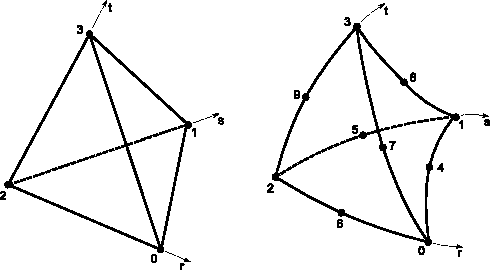
\includegraphics[width=8.5cm]{Figures/Tet4and10.pdf}
\caption{Linear tetrahedron with 4 nodes (tet4) and quadratic tetrahedron with 10 nodes (tet10)}
\label{Tet4AndTet10Illustration}
\end{figure}


The isoparametric 4-node tetrahedron interpolates the position linearly between the nodes (Fig. \ref{Tet4AndTet10Illustration}). Consequently, the stress is constant over the element and the element shows significant volumetric locking for nearly incompressible materials \cite{Belytschko2000}. In contrast, the 10-node tetrahedron interpolates positions with 2nd order polynomials and doesn't suffer from severe volume locking. Thus, in the realm of mechanical engineering it is well known that quadratic tetrahedra perform much better than linear tetrahedral meshes in many scenarios \cite{Cifuentes1992}. This is especially true for the simulation of incompressible objects.

Typically, the shape functions are defined in a local coordinate system $(r,s,t)$ and all element based operations such as calculating deformations, extracting rotations or numerical integration are performed in this local coordinate system. Polynomial functions (\emph{shape functions}) are used to map the local coordinates to the global coordinate system. If the polynomial degree of the shape functions matches the order of the basis functions, the element is called isoparametric. In case of the isoparametric 10-node tetrahedron, the shape functions are quadratic, which allows curved boundaries and therefore better approximation of the geometry (Fig. \ref{Tet4AndTet10Illustration}). 

As previously mentioned, the integrals that arise during the computation of the forces and the stiffness matrix are evaluated numerically. One cubature point per element is sufficient in order to integrate the stiffness matrix term eq. (\ref{CoRotStiffnessMatrix}) if linear basis functions are used. In contrast, four sample points are necessary to integrate the 10-node tetrahedron. Consequently, four rotation matrices have to be extracted per element for accurate integration. Alternatively, it is possible to extract just one rotation matrix per element by only using the four corner vertices in order to compute the deformation gradient. In this case the element matrix can be pre-computed and the numerical integration can be omitted, which reduces the computational costs by 75\%. This simplification will be referred to as the single rotation quadratic tetrahedron.


\subsection{Numerical validation}

Numerical simulation studies on a simple beam geometry are performed in order to compare the efficiency of the linear tetrahedral (tet4), the quadratic tetrahedral (tet10) as well as the single rotation quadratic tetrahedral (tet10SR) elements. In the first scenario, the beam deforms under gravity, while it is subjected to a twisting deformation pattern in the second scenario (Fig. \ref{BeamTwistAndGravity}). Incompressible material models (Poisson's ration $\nu=0.49$) are used throughout the study. The linear and the quadratic corotated FEM were implemented using the Simulation Open Framework Architecture (SOFA) toolkit \cite{Faure2012}. For all simulations in this study, the Newmark time integration scheme is used along with the Pardiso direct sparse solver from the Intel MKL 10.3.

\begin{figure}
   \centering   
   \psfragfig[width=0.98\textwidth]{Figures/BeamTwistAndGravity}
	\caption{Deformation under gravity (a) and twisting deformation pattern of a beam (b). A 1461 DOF tet4 mesh is compared to a 714 DOF tet10 mesh. The tet10SR element fails to capture the rotation at low resolution (b, middle), but achieves similar accuracy to the tet10 element at higher resolution (b, right).}
\label{BeamTwistAndGravity}
\end{figure}

In order to perform a quantitative analysis of the discretization error for each model, a reference solution on a high resolution quadratic mesh (100k elements) is computed for both problems. Test models of different resolutions are subsequently compared to this reference model.  We choose the root mean squared (RMS) error at the nodes of the reference solution as the error measures. The RMS errors with respect to the degrees of freedom (DOF) are depicted in Fig. \ref{ConvergenceQuadraticBeam}.

\begin{figure}
   \centering   
   \psfragfig[width=0.98\textwidth]{Figures/ConvergenceQuadraticBeam}
	\caption{RMS error over DOF for twisting deformation (left) and gravity induced deformation (right). The tet10 (green) and tet10SR (blue) elements show far superior accuracy for the same DOF than the tet4 (red) mesh.}
\label{ConvergenceQuadraticBeam}
\end{figure}

In case of the gravity induced deformation, tet4 elements need much more DOF (up to 40x) than tet10 elements in order to achieve the same accuracy. This result illustrates the locking behavior of linear tetrahedral elements. It should also be pointed out that the tet10SR formulation shows only negligible difference to the fully integrated tet10 element. Due to the displacement boundary conditions and the absence of volumetric forces, the difference in the twisting scenario is not as pronounced. However, the tet4 elements still need an order of magnitude more DOFs. It is apparent from Fig. \ref{BeamTwistAndGravity} that the tet4 mesh with 1461 DOFs still shows visible edges, while the lower resolution tet10 mesh (714 DOFs) produces a smooth deformation. It can also be seen that the tet10SR element fails to capture the rotations at low resolution (Fig. \ref{BeamTwistAndGravity}), but achieves a similar accuracy as the tet10 element for higher resolutions (right). It can be concluded that quadratic elements are superior to tet4 elements in both scenarios. Furthermore, the single rotation quadratic tetrahedral formulation (tet10SR) can be a computationally efficient alternative to the standard tet10 formulation for many applications.

%\setchapterpreamble[or][.5\textwidth]{%
\dictum[ Donald E. Knuth]{%
Science is what we understand well enough to explain to a computer. Art is everything else we do.}\vskip1em}



\chapter{Fast GPU-based finite element solver}
%\epigraphhead[5]{\epigraph{ Science is what we understand well enough to explain to a computer. Art is everything else we do. }{Donald E. Knuth}}		

In this chapter, we present a set of novel methods to efficiently simulate corotated quadratic FE models in real-time. First, we address the problem how high resolution surface meshes can be mapped to quadratic isoparametric elements. In this scenario, the difficulty arises from the fact that the mapping from the reference element to each quadratic element is not bijective and not analytically invertible. Furthermore, there are far less elements in a higher order FE mesh than in a linear mesh if compared in terms of DOF. Therefore, it becomes more important to accurately extrapolate deformations to surface points outside the FE mesh. In this chapter, we present a novel mapping scheme to overcome this problem.

Massively parallel hardware (so called general purpose graphics processing units - GPGPU) have become a popular choice in recent years for speeding up time-critical algorithms in the realm of image processing and simulation. Although this hardware type offers a significantly higher performance in terms of floating point operations per second than traditional CPU architectures, the algorithms have to be carefully designed in order to fully exploit these resources. In particular, the algorithm has to be heavily parallelizable. In the following, an efficient GPU based solver for quadratic corotated tetrahedra is presented. For this purpose, we first introduce a matrix-free scheme in order to facilitate the implementation of a GPU based conjugate gradient (CG) solver. Then, we show how the performance of this solver can be greatly enhanced by using a parallel preconditioner based on the factorized sparse approximate inverse (FSAI). Finally, we present a novel GPU-based multigrid scheme to efficiently solve elasticity models on higher order, unstructured, non-conforming grids.

\section{Accurate surface embedding for higher order finite elements}
\label{AccurateSurfaceEmbeddingSection}

In this section a novel approach to accurately map highly detailed surface meshes to a higher order FE computational mesh is presented. The novel mapping scheme relies on a representation of each surface vertex in terms of a point on the computational mesh and its distance to the FE mesh in normal direction. Through this representation, the surface deformations remain smooth and local shape features are preserved even if very low-resolution FE meshes are used for computation. An efficient algorithm based on non-linear optimization is proposed to construct the mapping. We show that the algorithm performs robustly and that its numerical complexity is linear in the number of surface nodes and constant in the number nodes in the computational mesh.

The following description and evaluation of the novel mapping scheme is based on the corresponding proceedings publication \cite{Suwelack2013}.


\subsection{Closest point search in higher order meshes}

In order to facilitate the computation of the mapping later on, we first detail an efficient scheme to compute the closest point $\mbp (r,s,t)$ in the FE mesh $\mMesh$ for each vertex $\mVert$ of the triangular surface mesh $\mSMesh$. We will first show how to find $\mbp(r,s,t)$ for a single given vertex $\mVert$. Based on this results, a recursive mapping scheme will be introduced that can be used to compute $\mbp(r,s,t)$ for all $\mVert$ in $\mSMesh$.


The distance $d(r,s,t)$ from a point $\mbp(r,s,t)$ in the element $\mElem$ to an arbitrary surface vertex $\mVert$ is given by
\begin{equation}
d(r,s,t) = \left\| \mVert - \mathbf{x}_I N_I(r,s,t) \right\|.
\label{DistanceComputation}
\end{equation}


As $\mVert$ can be outside of $\mElem$, we have to constrict $(r,s,t)$ such that $\mbp(r,s,t)$ is indeed in $\mElem$. We can thus formulate the closest point search in terms of the constrained optimization problem 
\begin{align}
	&\min d(\mbp(r,s,t)) \quad \textnormal{s.t.} \nonumber \\
	&r>0, s>0, t>0 \quad \textnormal{and} \quad r+s+t \leq 1.
	\label{ConstrainedProblem}
\end{align}

As previously mentioned, the solution to this problem can be analytically determined if linear shape functions are used. For higher order shape functions, non-linear programming techniques have to be employed. We solve the constrained optimization problem (eq. X\ref{ConstrainedProblem}) using an extended Levenberg-Marquardt algorithm \cite{Nocedal1999} \cite{Kanzow2005}. The Jacobian is calculated using finite differences. It is important to point out that simple Newton-Raphson iterations are not guaranteed to converge even in the unconstrained case when $\mVert$ is inside $\mElem$.

The solution to problem (\ref{ConstrainedProblem}) can be described as the local optimum for $\mbp (r,s,t) \in \mElem$. The next step is to find the element $\mElem_{\min}$ where $\mbp (r,s,t)$ reaches its global minimum distance $d_{\min}$ in $\mMesh$. This can be efficiently accomplished with a recursive algorithm (see algorithm \ref{PointRecursionAlgo}).


\begin{algorithm}  
\caption{Recursively find $\mbp(r,s,t) \in \mMesh$}
\label{PointRecursionAlgo}
  \begin{algorithmic}
  % \Require Starting Element $\mathbb{E}_0$
	\Procedure{ClosestPoint}{$\mVert, \mElem, d_{\min}, \mElem_{\min}, \mathcal{T}$ }
	\State Solve (\ref{ConstrainedProblem}) to find closest point $\mbp$ with distance $d$
	\State to $\mVert$ in $\mElem$
	\If{$d < d_{\min}$}		
	\State $d_{\min} = d$, $\mElem_{\min} = \mElem$		
	\EndIf
	
	\If{$\mbp$ is on face of $\mElem$}
		\If{$\mbp$ is on surface of $\mMesh$}
			\If{$\mbp$ is on surface edge}
				\State Find neighbour tetrahedron $\mElem_1$ that contains
				\State surface triangle which shares edge				
				\EndIf
		\Else			
			\State Find tetrahedron $\mElem_1$ that shares face

		\EndIf
	
	
				\If{$\mElem_1$ exists and $\mElem_1 \notin \mathcal{T}$}				
				\State Add $\mElem_1$ to $\mathcal{T}$
				\State \Call{ ($\hat \mbp, \hat d, \hat{\mElem}$) = ClosestPoint}{$\mVert, \mElem_1, d_{\min}, \mElem_{\min}, \mathcal{T}$} 	
					\If{$\hat d < d_{\min}$}		
				\State $d =  \hat d$, $\mElem = \hat{\mElem}$, ${\mbp} = { \hat \mbp}$				
				\State $d_{\min} = d$, $\mElem_{\min} = \mElem$		
				\EndIf
			\EndIf
			
			\EndIf
	
			\Return $\mbp,d, \mElem$
			\EndProcedure
		
  \end{algorithmic}
\end{algorithm}

We first select an element $\mElem$ to start the iteration. Subsequently the closest point $\mbp \in \mElem$ to $\mVert$ is computed. This procedure is recursively called on the neighboring tetrahedra, if $\mbp$ is on a face of $\mElem$. The recursion is aborted if $d=0$ (i.e. $\mbp$ is inside the current tetrahedron) or if the neighbor tetrahedron that shares the face has already been visited (i.e. is in set $\mathcal{T}$). During each recursion step, the minimum distance $d_{\min}$ in $\mElem_{\min}$ is updated if a closer point $\hat \mbp$ is found.

The algorithm efficiently computes the local minimum distance $d_{\min}$ for a given initial guess $\mElem$. This local minimum coincides with the global minimum if the initial guess $\mElem$ is close enough to the real solution.




\subsection{Recursive mapping scheme}			

We now seek to not only map the whole surface mesh $\mSMesh$ to the computation grid, but also to reliable find the global minimum $d_{\min}$ for all $\mElem_i \in \mMesh$. For this purpose we introduce an outer recursion to the presented algorithm \ref{PointRecursionAlgo}. An initial mapping correspondence is established by finding the closest surface vertex $\mVert_0$ in $\mSMesh$ for an arbitrary point $\mbp_0$ in $\mElem_0$. It is important to point out that this inverse mapping problem is much easier to solve as the resolution of $\mSMesh$ is much higher than the resolution of $\mMesh$.

In order to start the outer recursion, we arbitrarily select an initial triangle $\mTri_0$ that contains $\mVert_0$. We than start a recursive scheme which maps all points in a given triangle $\mTri$ and uses the current mapping results ($\mbp, \mElem$) as the initial guess for mapping the neighbor triangles of $\mTri$ (see algorithm \ref{TriangleRecursionAlgo}).


\begin{algorithm}  
\caption{Recursively map triangles in $\mSMesh$}
\label{TriangleRecursionAlgo}
  \begin{algorithmic}
  % \Require Starting Element $\mElem_0$
	\Procedure{MapTriangle}{$\mTri, \mElem, d_{t}, \mathcal{P}$ }
	\State triangleMapped = true
	\ForAll{Surface vertices $\mVert$ in $\mTri$} 
	\If{$\mVert \notin \mathcal{P}$}
	\State Initialize empty $\mathcal{T}$, $d_{\min} = \inf$
	\State \Call{ ($ p,  d, \hat{\mElem}$) = ClosestPoint}{$\mVert, \mElem, d_{\min}, \mElem_{\min}, \mathcal{T}$} 		
	\If{$d<d_t$}
		\State $\mElem = \hat{\mElem}$ 
		\State Map vertex $\mVert$ to point $p$ in $\mElem$
		\State Add $\mVert$ to $\mathcal{P}$		
	\Else
		\State triangleMapped = false
	\EndIf	
	\EndIf
	\EndFor
	\If{triangleMapped}
	\ForAll{Neigbour triangles $\mTri_n$}
	\State \Call{ MapTriangle}{$\mTri_i, \mElem, d_{t}, \mathcal{P}$}
	\EndFor	
	\EndIf
	\Return
	\EndProcedure
		
  \end{algorithmic}
\end{algorithm}

The initial guess for each triangle depends on the mapping order of the triangles. Thus, there might be mapping orders that don't generate initial guesses which guarantee a global optimum for $d_{\min}$. That's why the mapping order is controlled by introducing the distance threshold $d_{t}$. The triangle $\mTri$ is only mapped (and the recursion only continues) if the distance for each surface vertex in $\mTri$ is below $d_{t}$. In order to make sure that all triangles are mapped, this distance threshold is incrementally raised until all triangles are mapped. 

For implementation purposes, the recursive scheme has to be unrolled into a loop in order to ensure an efficient and stable computation for large meshes.

\subsection{Accurate surface embedding}


We now define a scheme that maps the surface mesh $\mSMesh$ onto the computational mesh $\mMesh$ such that the deformed surface $\mSMesh'$ can be extrapolated from the deformed FE mesh $\mMesh'$ in a fast and correct way. For this purpose we represent each surface model vertex $\mVert$ in terms of a point $\mbp$ on the FE grid and its distance $d$ in normal direction (see Fig. \ref{MethodIllustration}). The deformed vertex position  
\begin{equation}
\mVert ' = \mbp ' + d \mbn '
\end{equation}
can subsequently be constructed using the position of $\mbp$ in the deformed configuration ($\mbp '$) as well as the deformed normal $\mbn '$. It will become apparent from the numerical examples that the proposed mapping preserves the smoothness of the deformation (and thus local shape features) even for surface regions that lie outside of the computational mesh.

\begin{figure}
   \centering   
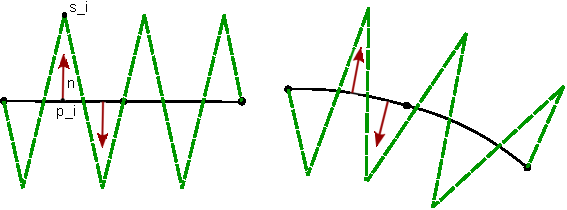
\includegraphics[width=\textwidth]{Figures/Seasaw.pdf}
\caption{Sawtooth surface attached to 1D quadratic edge. The deformation of the edge can be extrapolated to the surface while preserving local shape features.}
\label{MethodIllustration}
\end{figure}

\subsection{Smooth normal field}

At any surface point $\mbp$ on the mesh given in local coordinates $r, s$ with respect to the quadratic surface triangle, the spatial derivatives 
\begin{equation}
\frac{\partial \mbx (\mbp)}{\partial r} = \mathbf x_I \frac{\partial N_I (r,s)}{\partial r} \quad , \quad \frac{\partial \mathbf x (\mbp)}{\partial s} = \mathbf x_I \frac{\partial N_I (r,s)}{\partial s}
\end{equation}
can be calculated using the position of the nodes and the shape function derivatives at $r, s$ of the 6 node quadratic triangle. The normal $\mbn$ at $\mbp$ is then given by
\begin{equation}
\mbn  = \left( \frac{\partial \mathbf x (\mbp)}{\partial r} \times \frac{\partial \mathbf x (\mbp)}{\partial s} \right)/  \left\| \frac{\partial \mathbf x (\mbp)}{\partial r} \times \frac{\partial \mathbf x (\mbp)}{\partial s}  \right\|.
\label{NormalComputation}
\end{equation}

A smooth normal field is a necessary condition for the smoothness of the proposed mapping scheme. As the FE mesh is only $C^0$-continuous, the partial derivatives (and thus the normals) are discontinuous at element boundaries. Therefore, we average the normal at each node using the angle weighted average scheme. This results in an averaged normal $\overline{\mbn}_I$ for each surface vertex of the FE mesh and the normal 
\begin{equation}
\mathbf n  = ( \overline{\mbn}_I N_I(r, s) ) / \left\| \overline{\mbn}_I N_I(r, s) \right\|
\end{equation}
can be interpolated using the standard shape functions of the quadratic triangle. The smooth normal field that is created in this way can be efficiently computed. Furthermore, it is not necessary to re-compute the deformed vertex normals $\overline{\mbn}_I '$ every time step as shown in eq. (\ref{NormalComputation}). Instead, nodal rotation matrices can be defined at each node of the FE mesh which can be used to rotate the normal into the deformed configuration.


\subsection{Normal correction}

The aforementioned representation of each surface vertex $\mVert$ in terms of $(\mbp, d)$ can be obtained by solving a global optimization problem. The solution to this problem is not necessarily unique for complex, non-convex meshes. In order to construct the representation we first find the closest point $\mbp \in \mMesh$ to $\mVert$. Due to the normal smoothing, the normal $\mbn$ at $\mbp$ does not necessarily point in the direction of $\mVert$. Thus, we perform an additional correction step to make sure that the normal $\mbn$ at $\mbp$ does indeed point in the direction of $\mVert$. For this purpose we define the difference vector

\begin{equation}
\mathbold{\delta}(r,s,t) =  v_i - ( \mathbf{x}_I N_I(r,s,t) + d \cdot \mathbf{\overline{n}}_I N_I(r,s,t) ),
\label{NormalCorrectionComputation}
\end{equation}

where $d$ denotes the distance as defined in eq. (\ref{DistanceComputation}). The correction step can then be formulated in terms of the minimization problem 

\begin{align}
	&\min \mathbold{\delta}(r,s,t) \, \textnormal{s.t.} \nonumber \\
	&r>0, s>0, t>0 \, \textnormal{and} \, r+s+t \leq 1.
	\label{CorrectionProblem}
\end{align}

The optimization problem is solved in the same way as problem (\ref{ConstrainedProblem}): A recursive scheme along the lines of algorithm \ref{PointRecursionAlgo} is employed on top of a constrained Levenberg-Marquardt optimizer that uses finite differences to approximate the Jacobian.


\section{Matrix free conjugate gradient solver}

The necessary steps for solving the fully discretized scheme of the dynamic corotational formulation have already been outlined in section \ref{SectionProjectionBaedConstraints}. From this scheme, three computationally significant steps can be extracted: The computation of the nodal forces, the assembly of the stiffness matrix and the linear system solve. 


The nodal force computation consists of two stages. First, the elemental rotations are extracted and the elemental stiffness matrices are obtained through numerical integration. Afterwards, the elemental contributions are added to the nodal force vector. The whole process is inherently parallel and can be easily implemented on the GPU. In accordance with previous work (e.g. Allard et al. \cite{Allard2011}) we use one kernel launch to perform the elemental computations such as the polar decomposition of the deformation gradient and an additional kernel launch for the per-vertex gather operation. 


Implementing the matrix assembly and system solve step on the GPU is much more difficult. Most linear solvers (in particular the direct ones) do not parallelize well. For symmetric and positive definite systems an exception exists in the form of the conjugate gradient (CG) approach. This iterative method describes the linear system solve as a minimization problem for convex quadratic functions. The core ideas is to use so called conjugate directions instead of the local gradient for an efficient gradient descent minimization scheme \cite{Nocedal1999}. 


\begin{algorithm}  
\caption{Conjugate gradient algorithm for solving $\mathbf A \mathbf x = \mathbf b$}
\label{CGAlgo}
  \begin{algorithmic}
  % \Require Starting Element $\mathcal{E}_0$
	\State set $\mathbf x_0=0, \mathbf r_0 = \mathbf A \mathbf x_0- \mathbf b, \mathbf p_0 = -\mathbf r_0, k=0$ 
	\For{$k=0 < \textnormal{maxIter}$ } 
	\If{$\left\| \mathbf{r}_k \right\| / \left\| \mathbf{b} \right\| < \epsilon$}
		\State{break}
	\EndIf
	\State{$\alpha_k = \dfrac{\mathbf{r}^T_k \mathbf{r}_k}{\mathbf{Z}^T_k \mathbf{A} \mathbf{Z}_k} $ } 
	\State{$\mathbf x_{k+1} = \mathbf x_{k} + \alpha \mathbf p_{k}$} 
	\State{$\mathbf r_{k+1} = \mathbf x_{k} + \alpha \mathbf A \mathbf p_{k}$} 
	\State{$\beta_{k+1}=\dfrac{\mathbf{r}^T_{k+1} \mathbf{r}_{k+1}}{\mathbf{r}^T_k \mathbf{r}_k}$}
	\State{$\mathbf{Z}_{k+1} = -\mathbf{r}_{k+1}+\beta_{k+1} \mathbf{Z}_{k} $}
	\State{k=k+1}
	\EndFor
  \end{algorithmic}
\end{algorithm}


A basic sketch of the CG scheme (see Alg. \ref{CGAlgo}) reveals that only simple computational tasks such as vector addition, vector-vector multiplication and a (sparse) matrix-vector product are necessary for the system solve. In the context of an efficient GPU implementation, the most challenging part is the sparse matrix-vector product (SpMV) between the system matrix (see eq. \ref{LinearSystemNewmark}) and the current search direction $p_k$ in each CG step. In order to avoid a time-consuming matrix assembly, we don't build the system matrix every time step, but instead use a similar approach as Allard et al. \cite{Allard2011}: We first compute the per-element contributions for each nodal force and then accumulate these results for each node. In contrast to Allard et al. (and in contrast to the procedure for computing the nodal forces), we don't use a separate kernel launch for the per-vertex operations. Instead, we use a multi-coloring technique such that primarily those elements who do not share a common node are processed in parallel. With our layout it is still possible (although very rare) that the nodal force contributions of two elements of different color are updated simultaneously. We thus use an atomic operation in order to add these contributions to the nodal forces. As the atomic add causes virtually no overhead when no write conflicts occur, it is very efficient when used in combination with coloring techniques. 

The elemental contributions are computed by multiplying dense elemental matrices with corresponding nodal vectors. The performance of this kernel is limited by the memory bandwidth. In order to reduce the data transfer to global memory and to reduce the amount of shared memory used by each thread, we exploit the symmetry of the elemental matrices and use compressed matrices for data transfer. The matrix vector product is then performed using a constant lookup table for index mapping between the compressed and the uncompressed matrix.


\section{FSAI preconditioned conjugate gradients}
\label{PCGSection}

For inhomogeneous and stiff materials, the discrete elasticity problem becomes increasingly ill-conditioned, i.e. the condition number

\begin{equation}
\kappa (\mathbf{A}) = \left\| \mathbf{A} \right\|\cdot \left\| \mathbf{A}^{-1} \right\|
\end{equation}

becomes large. In this case, pure CG methods converge very poorly. A proven solution to this problem is to apply a preconditioner $\mathbf{Z}$\footnote{often denoted with $\mathbf P$ in the literature, we use $\mathbf Z$ to avoid confusion with the first Piola-Kirchhoff stress tensor} to the linear system. It is immediatly clear from  
\begin{equation}
\mathbf{Z}^{-1} \mathbf{A} \mathbf{dx} = \mathbf{Z}^{-1} \mathbf{b}
\end{equation}

that if $\mathbf{Z}^{-1}$ is close to $\mathbf{A}$, then $\mathbf{Z}^{-1}\mathbf{A}$ is near the identity matrix and the condition number $\kappa$ is low. If a preconditioner is used in a CG scheme, it has to be applied in each iteration, i.e. the equation

\begin{equation}
 \mathbf{Z} \mathbf{r} = \mathbf{z}
\label{PrecondApplication}
\end{equation}

has to be solved for the temporary vector $\mathbf{r}$ and the right hand side $\mathbf{z}$. That is why a key requirement for a good preconditioner is that its application according to eq. (\ref{PrecondApplication}) is fast and efficient. The Jacobi preconditioner therefore simply scales $\mathbf{A}$ with its inverse diagonal which means it uses the preconditioner $\mathbf{Z} = \textnormal{diag}(\mathbf{A})$.

A family of powerful preconditioners arises from the decomposition of $\mathbf{A}$ into triangular matrices. Every arbitrary square matrix can be written as the product of a lower and upper triangular matrix (LU decomposition). For symmetric, positive definite matrices the incomplete Cholesky (IC) decomposition 
\begin{equation}
\mathbf{A} \approx \mathbf{L}_A \mathbf{L}_A^T = \mathbf{Z}
\end{equation}

can drastically reduce the number of CG iterations for elastic problems \cite{Courtecuisse2010}. The application of the IC preconditioner requires two triangular solves of the sparse triangular matrices $\mathbf{L}_A,\mathbf{L}_A^T$. While this can be very efficient on the CPU, the triangular solve is inherently recursive, which makes a GPU implementation difficult.

The factorized sparse approximate inverse (FSAI) preconditioner is based on a different idea \cite{Kolotilina1993}. This method seeks to directly approximate the inverse of $\mathbf{A}$. In order to achieve this goal, $\mathbf{A^{-1}}$ is decomposed according to 

\begin{equation}
\mathbf{A^{-1}} \approx \mathbf{G}_L ^T \mathbf{G}_L = \mathbf{Z}^{-1}.
\end{equation}

In this context, the matrix $\mathbf{G}_L$ is an approximation the inverse of the lower Cholesky factor $\mathbf{L}_A$ in terms of the Frobenius norm $\left\| \mathbf{I}- \mathbf{G}_L \mathbf{L}_A  \right\|_F$. The approximation is constructed by minimizing the aforementioned Frobenius norm for a given sparsity pattern of $\mathbf{G}_L$. The commonly used FSAI(q) method uses the sparsity pattern of $\left| \mathbf{A} \right| ^q$.

The application of the FSAI preconditioner only needs two SpMV operations which are very fast on the GPU. It is clear that the more fill-ins are allowed in a higher order FSAI(q) scheme, the better is the approximation to $\mathbf{A^{-1}}$. However, at the same time the SpMV becomes increasingly time-consuming to compute. 

The biggest drawback of the FSAI preconditioner is its high set-up time. In the next section we describe how to overcome this problem.


\subsection{Preconditioner warping}
\label{PreconditionerWarping}
In the context of interactive simulations it is not feasible to compute the preconditioner every timestep, especially if complex schemes such as IC or FSAI are used. A better strategy is to compute the preconditioner just once and then appropriately adapt it every time step. For elasticity problems based on the corotated formulation, this can be efficiently achieved by local rotation warping of the preconditioner \cite{Courtecuisse2010}. The idea is based on the fact that the change in the system matrix $\mathbf{A}$ is dominated by the rotation warping of the elemental stiffness matrices (eq. \ref{CoRotStiffnessMatrix}). 

In order to apply these rotations to $\mathbf{Z}^{-1}$, we extract a local rotation $\mathbf{R}_n$ per node. We can subsequently define the global block diagonal rotation matrix $\mathbf{R}$ to formulate

\begin{equation}
\mathbf{R} \mathbf{Z}^{-1} \mathbf{R}^T \mathbf{A} \mathbf{dx} = \mathbf{R} \mathbf{Z}^{-1} \mathbf{R}^T \mathbf{b}.
\end{equation}

It is important to note that we do not have to explicitly compute $\mathbf{R} \mathbf{Z}^{-1} \mathbf{R}^T$ for each timestep, instead we serially apply the three operators. In this case it is not even necessary to build the global matrix $\mathbf{R}$, but each node can instead be rotated using the $3\times3$ matrix $\mathbf{R}_n$.

In the corotated FE model, the rotations are extracted on a per element basis. In order to compute the nodal rotations, we average the elemental rotations for each element around the node. This is done by first averaging the deformation gradient at the node before performing the rotation extraction according to Higham et al. \cite{Higham1988}. We have found this procedure to be more efficient than directly averaging the rotations using quaternions. In the case of quadratic tetrahedra, we use only the 4 corner vertices to compute the deformation gradient as explained in section \ref{QuadraticTetrahedraSection}.

Thanks to the warping scheme, the FSAI preconditioner can be computed in a pre-processing step from the linear stiffness matrix. It is even possible to store the preconditioner to disk and just load it at the beginning of each simulation.

The GPU implementation of the rotation warping and the subsequent application of the FSAI preconditioner is straight forward as the process is inherently parallel with a high data locality. As described above the rotation warping is performed by simply multiplying each node with a $3\times3$ rotation matrix. The application of the FSAI preconditioner requires two SpMV products. As the FSAI matrices do not change during the simulation, we just store them in GPU memory and apply them using a suitable CUDA library. 


\section{GPU-based multigrid solver for unstructured, non-conforming meshes}

The computational effort for the preconditioned conjugate gradient approach does scale superlinearly in terms of the number of mesh nodes (i.e. the DOF): Not only does the computational time for each PCG iteration increase, but the number of PCG steps increases as well for a fixed residual threshold. Thus, the method becomes inefficient for high resolution models. In contrast, multigrid methods can keep the computational effort proportional to the number of mesh nodes. The core idea is to efficiently remove low frequency errors by solving the linear system on a hierarchy of grids with different resolutions.

In this section, we present a novel multigrid scheme for efficiently solving elasticity problems using higher order FE on unstructured, non-conforming grids. We furthermore outline a set of methods that allows to efficiently implement the scheme on massively parallel architectures. In the following, we first give a brief general introduction to geometric multigrid schemes for solving linear systems that arise from elliptic PDEs. In this context we especially highlight the necessary components of the approach. Based on this discussion, we present a suitable prolongation/restriction scheme and a highly parallel smoothing scheme for simulations on unstructured grids. Finally, we detail a multigrid-preconditioned CG solver for the real-time simulation of deformable models.


\subsection{Basic multigrid scheme}

At the core of a multigrid solver lies a hierarchy of problem discretizations of different resolutions. This hierarchy consists of $l_{\textnormal{max}}$ levels with the associated system matrices $\mathbf A _l$. The solution scheme starts with an initial guess $\mbx _0$ on level $l=0$. In practice $\mbx _0$ is often chosen to be a vector of zeros or a value from a previous time step. The high frequency errors in this solution are subsequently attenuated by applying the smoothing operator $\mathcal{S}$. Typically, a variant of a fixed point iteration is used for this purpose (see section \ref{GPUBasedSmoothingSection} for details). In order to eliminate the low frequency errors, the remaining residual is consequently transferred to the next level $l+1$ with lower resolution. To do so, the residual $\mathbf r_l$ is first computed on the level $l$ and then transferred to the lower resolution mesh using the restriction operator $\mathcal{R}$ (refer to section \ref{MultigridHierarchySection} for more information). If the maximal mesh level $l_{\textnormal{max}}$ is reached, the remaining error $\mathbf e_{l+1}$ is determined by solving $\mathbf A _{l+1} \mathbf e_{l+1} = \mathbf r_{l+1}$ on the coarser mesh. This can be either done with a direct solver or using an iterative method such as the previously presented preconditioned gradient approach. If $l+1 < l_{\textnormal{max}}$, then the residual equation is recursively solved on the remaining levels of subsequently coarser meshes. In both cases, the error correction $\mathbf e_{l+1}$ is then transferred to the finer mesh at level $l$ by means of the prolongation operator $\mathcal{P}$. After adding the correction term $\mathbf e_{l}$ to the solution, a final smoothing step removes high-frequency errors that are introduced by the prolongation process.

In practice, several variants of the described multigrid scheme are used. First of all, the number of levels $l_{\textnormal{max}}$ can vary depending on the application. Furthermore, the described V-cycle is usually repeated several times until a given residual threshold is met. Finally, in many applications it is more efficient to spend more solving time on the coarse grids, thus leading to so called W-cycles. For a more detailed discussion on the basics of geometric multigrid methods we refer to appropriate textbooks \cite{Braess2007}.  

\begin{algorithm}  
\caption{V-cycle multigrid scheme for solving $\mathbf A \mathbf x = \mathbf b$}
\label{MGAlgo}
  \begin{algorithmic}
	\Procedure{MultigridSolve}{$\mathbf x_0 , \mathbf b , l$ }
	\State{${\mbx} \leftarrow \mathcal{S} (\mbx _0, \mathbf A_l, \mathbf b )$}	
	\State{$\mathbf r_l = \mathbf A _l {\mbx} - \mathbf b $}
	\State{$ \mathbf r _{l+1} \leftarrow \mathcal{R} (\mathbf r _l)$}
		\If{$l+1 < l_{\textnormal{max}}$}
		\State{InnerSolve $\mathbf A _{l+1} \mathbf e_{l+1} = \mathbf r_{l+1}$} 
	\Else
		\State { MultigridSolve({$\mathbf e _{l+1}, \mathbf b _{l+1}, l+1$ })}
	\EndIf	
	\State{$\mathbf e _l \leftarrow \mathcal{P} (\mathbf e _{l+1})$ }
	\State{$\mbx = {\mbx} + \mathbf e _l  $ }
	\State{${\mbx} \leftarrow \mathcal{S} (\mbx, \mathbf A_l, \mathbf b )$}	
	\State \Return{ \mbx }
	\EndProcedure	
  \end{algorithmic}
\end{algorithm}

\subsection{Multigrid hierarchy for non-conforming, higher order meshes}
\label{MultigridHierarchySection}

An accurate transfer of quantities between the meshes in the grid hierarchy is key in order to achieve an efficient multigrid scheme. For elasticity problems, the prolongation operator interpolates displacements between the meshes. The restriction operator transfers forces from a finer to a coarser grid. In many applications for geometric multigrid methods (especially in the realm of computational fluid mechanics), the finer mesh levels are constructed from an initial coarse mesh. In this way, all mesh levels cover the same region $\Omega_0$ (conforming mesh hierarchy). A construction of suitable prolongation and restriction operators is thus straight forward. Typically, these operators are linear and therefore have a matrix representation. In this context, the restriction operator is often chosen to be the transpose of the prolongation scheme. 

In order to accurately solve elasticity problems on unstructured grids, it is important to approximate the geometry as closely as possible. It is thus not desirable to construct the grid hierarchy from a coarse initial mesh. Instead, each mesh in the hierarchy should approximate the geometry as best as possible. Consequently, the meshes do not entirely overlap (non-conforming hierarchy) and thus displacements have to be extrapolated. When using linear tetrahedral grids, this can be achieved using barycentric coordinates \cite{Georgii2008}.

As outlined in section \ref{AccurateSurfaceEmbeddingSection} the interpolation and extrapolation of displacement and force fields that are defined on higher order isoparametric grids is more challenging. In our multigrid scheme, we use the previously presented mapping scheme based on the surface normal in order to interpolate the displacement between meshes (prolongation). In order to restrict the residual force vector to a coarser mesh, we do not make use of the surface normal. Rather, we map each nodal force to the corresponding element $\mElem$ in the coarse mesh that contains the closest point $\mbp (r,s,t)$ to the node. This force is then distributed among the nodes of $\mElem$ according to the basis function values at $\mbp (r,s,t)$.


\subsection{GPU-based smoothing}
\label{GPUBasedSmoothingSection}
The smoothing operators that are commonly used in geometric multigrid solvers can be expressed as fixed point iteration schemes. The idea of this class of iterative methods is to use the non-singular matrix $\mathbf B$ in order to express the linear system $\mathbf A \mbx = \mathbf b$ through
\begin{equation}
\mathbf B \mbx  + (\mathbf A - \mathbf B) \mbx = \mathbf b.
\end{equation}
The definition of the iteration 
\begin{equation}
\mathbf B \mbx ^{k+1}  + (\mathbf A - \mathbf B) \mbx^{k} = \mathbf b
\end{equation}
yields the update equation
\begin{equation}
\mbx ^{k+1} = \mbx^{k} - \mathbf B ^{-1} (\mathbf A \mbx^{k} - \mathbf b).
\label{MultigridUpdate}
\end{equation}

By decomposing $\mathbf A = \mathbf A_D + \mathbf A_L+ \mathbf A_U$ into the diagonal matrix $\mathbf A_D$ as well as the lower triangular matrix $\mathbf A_L$ and the upper triangular matrix $\mathbf A_U$, we can define two important smoothing schemes: Choosing $\mathbf B = \mathbf A_D$ yields the Jacobi method, while the Gauss-Seidel iteration scheme arises if $\mathbf B = \mathbf A_D + \mathbf A_L$. In a similar fashion as preconditioning techniques (see section \ref{PCGSection}), smoothing operators tend to work well, if $\mathbf B ^{-1}$ is a good approximation of $\mathbf A ^{-1}$. Thus, another class of commonly used smoothers are given by triangular decompositions of $\mathbf A$ such as $\mathbf B = \mathbf L \mathbf U$ (incomplete LU factorization) or $\mathbf B = \mathbf L \mathbf L^T$(incomplete Cholesky factorization).

It is apparent that the most efficient smoothers (e.g. Gauss-Seidel, ILU) rely on iteration schemes that are inherently recursive and thus not suitable for GPU implementation. For structured grids it is possible to divide the mesh into sets of non-neighboring elements (\emph{mesh coloring}) in order to parallelize the Gauss-Seidel method. However, this approach is very inefficient on unstructured grids. 

In order to facilitate a more efficient smoothing scheme, we use the previously presented FSAI technique ($\mathbf B^{-1} = \mathbf{G}_L ^T \mathbf{G}_L$). We again choose to precompute this decomposition and use the rotation warping technique to update the smoothing matrix for each time step. This results in a highly parallel algorithm that can be efficiently implemented on the GPU. In order to compute the SpMV product in the update equation (\ref{MultigridUpdate}), we again use the presented matrix-free scheme in order to avoid an assembly of the global system matrix.

\subsection{Multigrid-preconditioned CG for real-time elasticity}

We found that in many low-resolution elasticity problems, the prolongation leads to larger high-frequency errors near Dirichlet boundaries. Consequently, many smoothing steps are necessary, if the multigrid scheme is directly used for solving the linear system. An attractive alternative is to use the multigrid scheme as a preconditioner in a PCG algorithm. In this case, the accuracy of the multigrid iterations can be intentionally reduced. Thus it is enough to perform one V-cycle and 1 or 2 smoothing iterations within each preconditioning step. In order to achieve an efficient GPU implementation, we use the previously presented FSAI-preconditioned CG solver to perform the inner solve. Here, a residual threshold as high as 0.1 can be used without significantly degrading the performance of the solver. 


\section{Performance evaluations}

\subsection{Accurate surface embedding}

The novel mapping scheme was integrated into the SOFA framework \cite{Faure2012}. The constrained Levenberg-Marquardt implementation from the Levmar library was used to solve the minimization problem (eq. \ref{ConstrainedProblem}) \cite{LourakisJul.2004}. All simulations are run on a single core of an Intel i7-930 and we use nearly incompressible material models (Poisson's ratio $\nu=0.49$) in all scenarios.


\subsubsection{Accuracy}

The novel mapping scheme allows to accurately map high resolution surfaces to very low resolution quadratic tetrahedral grids. Fig. \ref{BunnySimulation} shows the deformation of the Stanford Bunny under gravity. It can be seen that the surface model mapped to a quadratic mesh with 1197 DOF deforms smoothly at the ears, although the computational mesh fails to approximate the geometry in this area. In contrast, the 9468 DOF tet4 model shows severe volume locking at the ears.

\begin{figure}
   \centering   
   \psfragfig[width=0.98\textwidth]{Figures/QuadraticTetrahedra/Bunny}
	\caption{Bunny surface mesh deforms under gravity. Volume locking is observed at ears for the simulation based on linear tetrahedra (left), while the tet10 mesh (middle) produces realistic and smooth surface deformations (right).}
\label{BunnySimulation}
\end{figure}

The gravity induced deformation of a seahorse model is considered as a second example. We construct different low resolution computational meshes from a high resolution surface mesh with 40k triangles: A linear tetrahedral (tet4) mesh with 258 DOF and 181 elements, a linear tetrahedral mesh with 992 elements and 1488 DOF as well as a mesh with 171 quadratic elements (tet10) and 1260 DOF (see Fig. \ref{SeahorseSimulation}). Barycentring coordinates are used in order to map the linear tetrahedral to mesh to the high resolution surface, while the presented mapping scheme is used to embed the tet10 mesh. As was apparent from the previous simulations of the beam geometry, linear meshes do not deform nearly as much as the quadratic FE mesh (volume locking effect). In order to ensure visually similar deformations, we thus subject the linear meshes to higher forces in order to overcome this artificial stiffness. 

\begin{figure}
   \centering   
   \psfragfig[width=0.98\textwidth]{Figures/QuadraticTetrahedra/SeahorseTet4AndTet10}
	\caption{Deformation of a seahorse model, from left to right: Linear tetrahedral FE mesh with 992 elements, the corresponding deformed surface mesh, a quadratic tetrahedral mesh with 171 elements and the deformed surface mesh mapped to the higher order FE mesh using the proposed mapping scheme.}
\label{SeahorseSimulation}
\end{figure}

For very low resolution tet4 meshes, the barycentric surface coupling results in large visible artefacts (see Fig. \ref{SeahorseSimulationCloseUp} left). In contrast, the proposed mapping scheme smoothly extrapolates the the deformation of the quadratic mesh is to the surface mesh and preserves local shape features. In case of the higher resolution tet4 mesh, the visible artefacts are substantially reduced. However, volumetric locking can still be observed at the end of the seahorse's tail. In contrast, the movement on the tail is much better captured by the quadratic mesh, also it has less DOF than the tet4 one (1260 vs. 1488). Furthermore, the barycentric mapping leads to a visible distortion of the seahorse's thorns even when using the higher resolution tet4 mesh (Fig. \ref{SeahorseSimulationCloseUp}). In contrast, the novel mapping scheme preserves the shape of the thorns. The dorsal fin of the seahorse is not included in the low resolution tet10 mesh and its deformation must thus be extrapolated during the simulation. Fig. \ref{SeahorseSimulationCloseUp} shows that this might lead to undesirable results even if the rotation invariant mapping is employed.


\begin{figure}
   \centering   
   \psfragfig[width=0.98\textwidth]{Figures/QuadraticTetrahedra/SeahorseCloseUp}
	\caption{Seahorse subjected to volumetric force: While the barycentric coupling leads to visible distortions (left, middle), the proposed mapping preserves local shape features (right).}
\label{SeahorseSimulationCloseUp}
\end{figure}


\subsubsection{Speed}

The performance and robustness of the approach is evaluated by mapping surface and volume meshes of different resolutions. We construct two volume meshes from the Asian dragon model that is included in the Stanford 3D scanning repository with 3000 elements and 1000 elements, respectively. Furthermore, surface models with mesh size from several thousands to several 100k elements are generated. The optimization algorithms robustly finds the correct surface representation (i.e. a point $\mbp$ on the computational mesh and the corresponding distance $d$) for all considered surface meshes. The convergence analysis (Fig. \ref{MappingConvergence}) confirms that the numerical complexity of the algorithm is linear in the number of surface nodes and independent of the size of the coarse computational mesh. 

Although the constrained Levenberg-Marquardt optimization that is run for each element is numerically complex, even large surface meshes with several 100k elements can be mapped in less than a minute thanks to the good convergence properties of the recursive scheme. Furthermore, the proposed surface representation can even be constructed in an offline process and the obtained coordinates can be simply loaded upon startup of the online simulation.

\begin{figure}
   \centering   
   \psfragfig[width=0.98\textwidth]{Figures/QuadraticTetrahedra/DragonConvergence}
	\caption{Different surface meshes are mapped to a 3000 element mesh (blue) and a 1000 element mesh (green). The mapping time is linear in the number of points of the surface mesh and independent of the computational mesh size.}
\label{MappingConvergence}
\end{figure}



\subsection{GPU based PCG solver}

The presented FSAI based GPU solver as well as Jacobi and ILU-preconditioned approaches were implemented using the SOFA framework \cite{Faure2012} and the Paralution library. All CPU computation are performed on a single core of an Intel i7-930, while the GPU implementation is run on a Tesla C2070. 

We again use the simple beam geometry under gravitational load (see Fig. \ref{BeamTwistAndGravity}) in order to assess the performance of the different solver configurations. We solve the dynamic problem with the Newmark integration method and scompute 200 time steps with a step size of $\Delta t = 0.05s$.

If the tet4 beam problem is solved using a CG-based scheme, the computation time of the nodal forces (right hand side) is negligible if compared to the linear system solve (see Fig. \ref{CGVsDirect}). For the 1461 DOF problem, the assembly of the nodal forces takes 10.39 ms on the CPU and the linear system solve is performed in 222.34 ms. Whereas for the smaller 1461 DOF problem only an acceleration factor of 1.3 is achieved by running the solver on the GPU, the large 58k DOF problem is solved more than 8 times faster on the GPU implementation. In case of the tet10 mesh, these observations are still valid, although the nodal force computations take about 10\% of the total solving time in this scenario. For this reason, the GPU speed-up is a bit higher for smaller problems (1.8x for the 2217 DOF beam). It can also be observed from Fig. \ref{CGVsDirect} that even the GPU-based Jacobi-preconditioned CG solver is heavily outperformed by the direct single-core Pardiso solver, which solves the 1461 DOF problem in 25 ms. 


\begin{figure}[htbp]
   \centering   
   \includegraphics[width=0.92\textwidth]{Figures/CGVsDirect.pdf}     
\caption{Solution times for the tet4 beam (top) and the tet10 beam (bottom). The complete solving time per time step for a Jacobi-preconditioned CG solver on the CPU (green) and on the GPU (red) is divided into the nodal force computations (dotted line) and the linear system solve (dashed line). Total solve time for the direct solver is shown in black.}
\label{CGVsDirect}
\end{figure}

As previously discussed, more complex preconditioners can speed up the CG scheme. Fig. \ref{PreconditionerComparison} shows that if an ILU preconditioner is used in conjunction with the presented rotation warping scheme, a speed-up by a factor of 3.6 can be obtained. Using the highly parallelizable FSAI approach leads to a speed-up of 1.7x in comparison to the Jacobi-preconditioned algorithm. For the purpose of real-time soft tissue registration it is not necessary to compute the exact solution of the linear system for each time step. By using a residual of 0.01 as the stopping criterion for the CG iterations, a sufficient accurate solution is obtained and the solution time can be significantly reduced (Fig. \ref{PreconditionerComparison} right). 

\begin{figure}[htbp]
   \centering   
   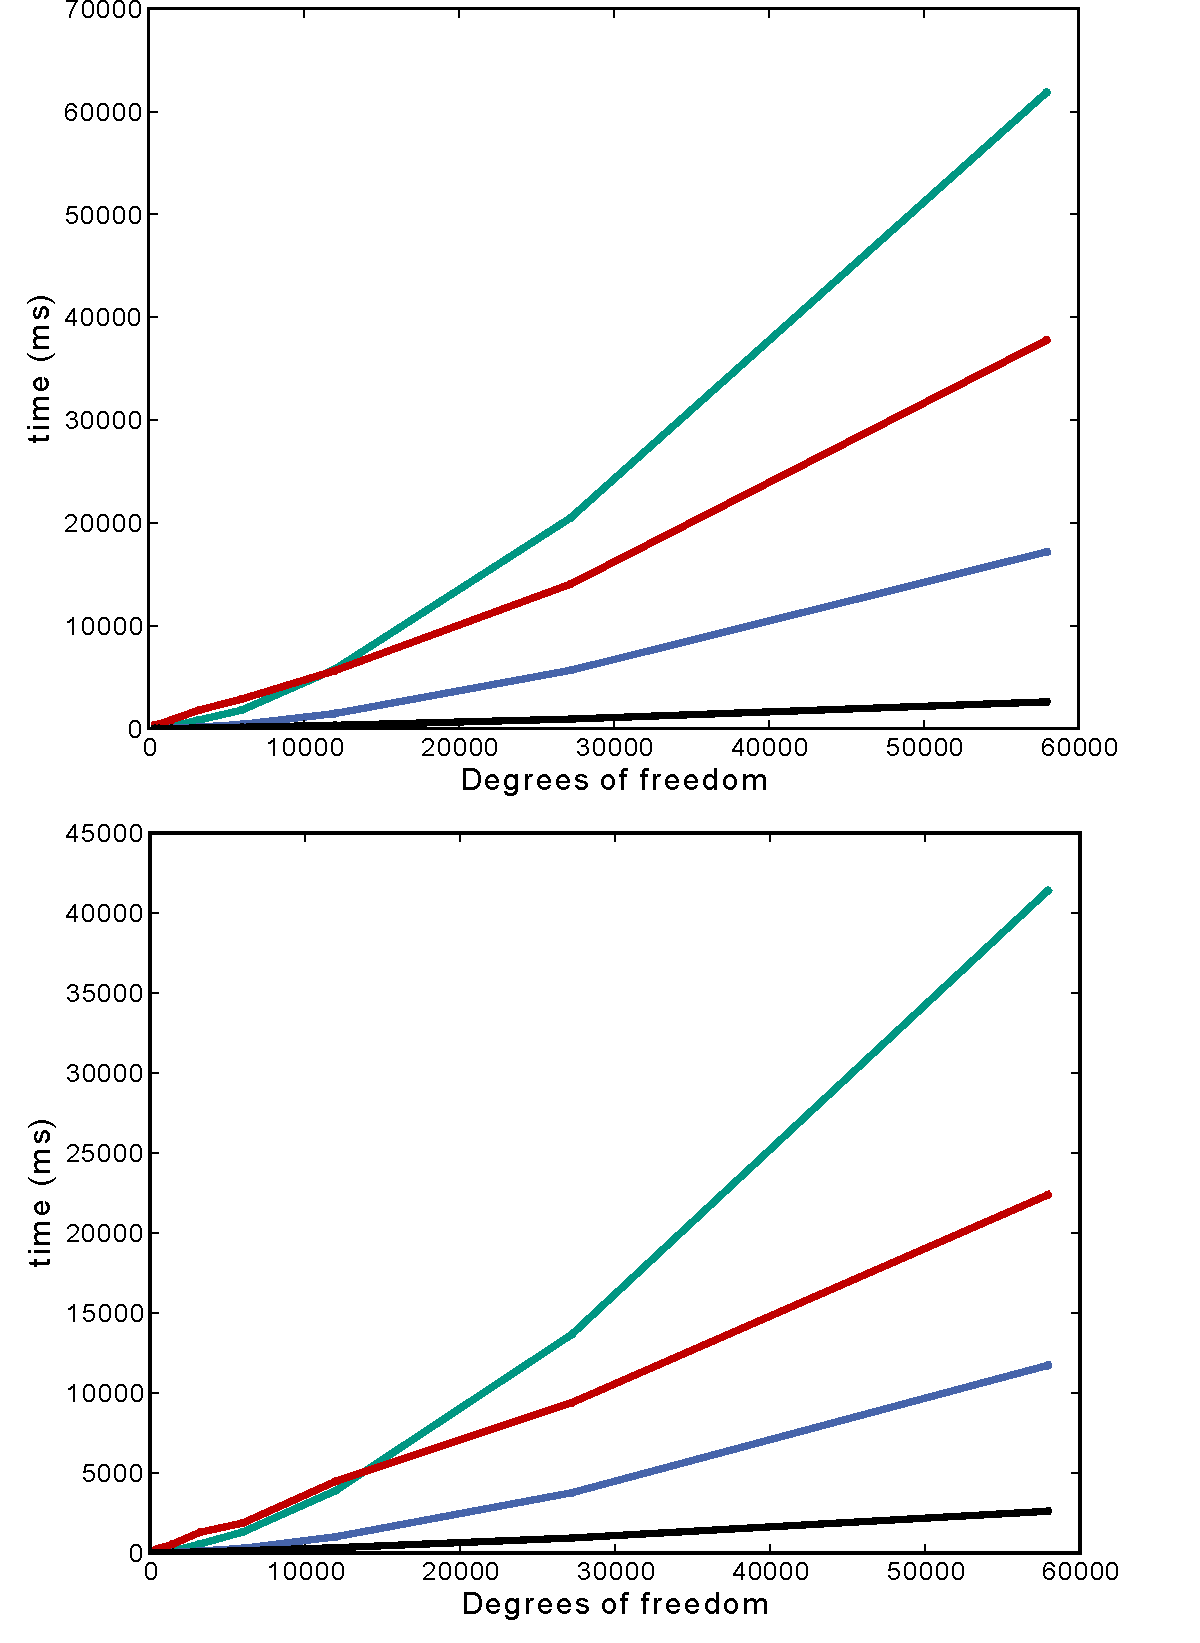
\includegraphics[width=0.92\textwidth]{Figures/PreconditionerComparison.pdf}     
\caption{Solution times for a CPU based CG solver scheme with a Jacobi (green), ILU (blue) and FSAI (red) preconditioner in comparison with a direct solver (black). The solution can be significantly speed up if a residual threshold of 1e-2 (bottom) is used for the CG scheme instead of computing the exact solution (top).}
\label{PreconditionerComparison}
\end{figure}



\begin{figure}[htbp]
   \centering   
   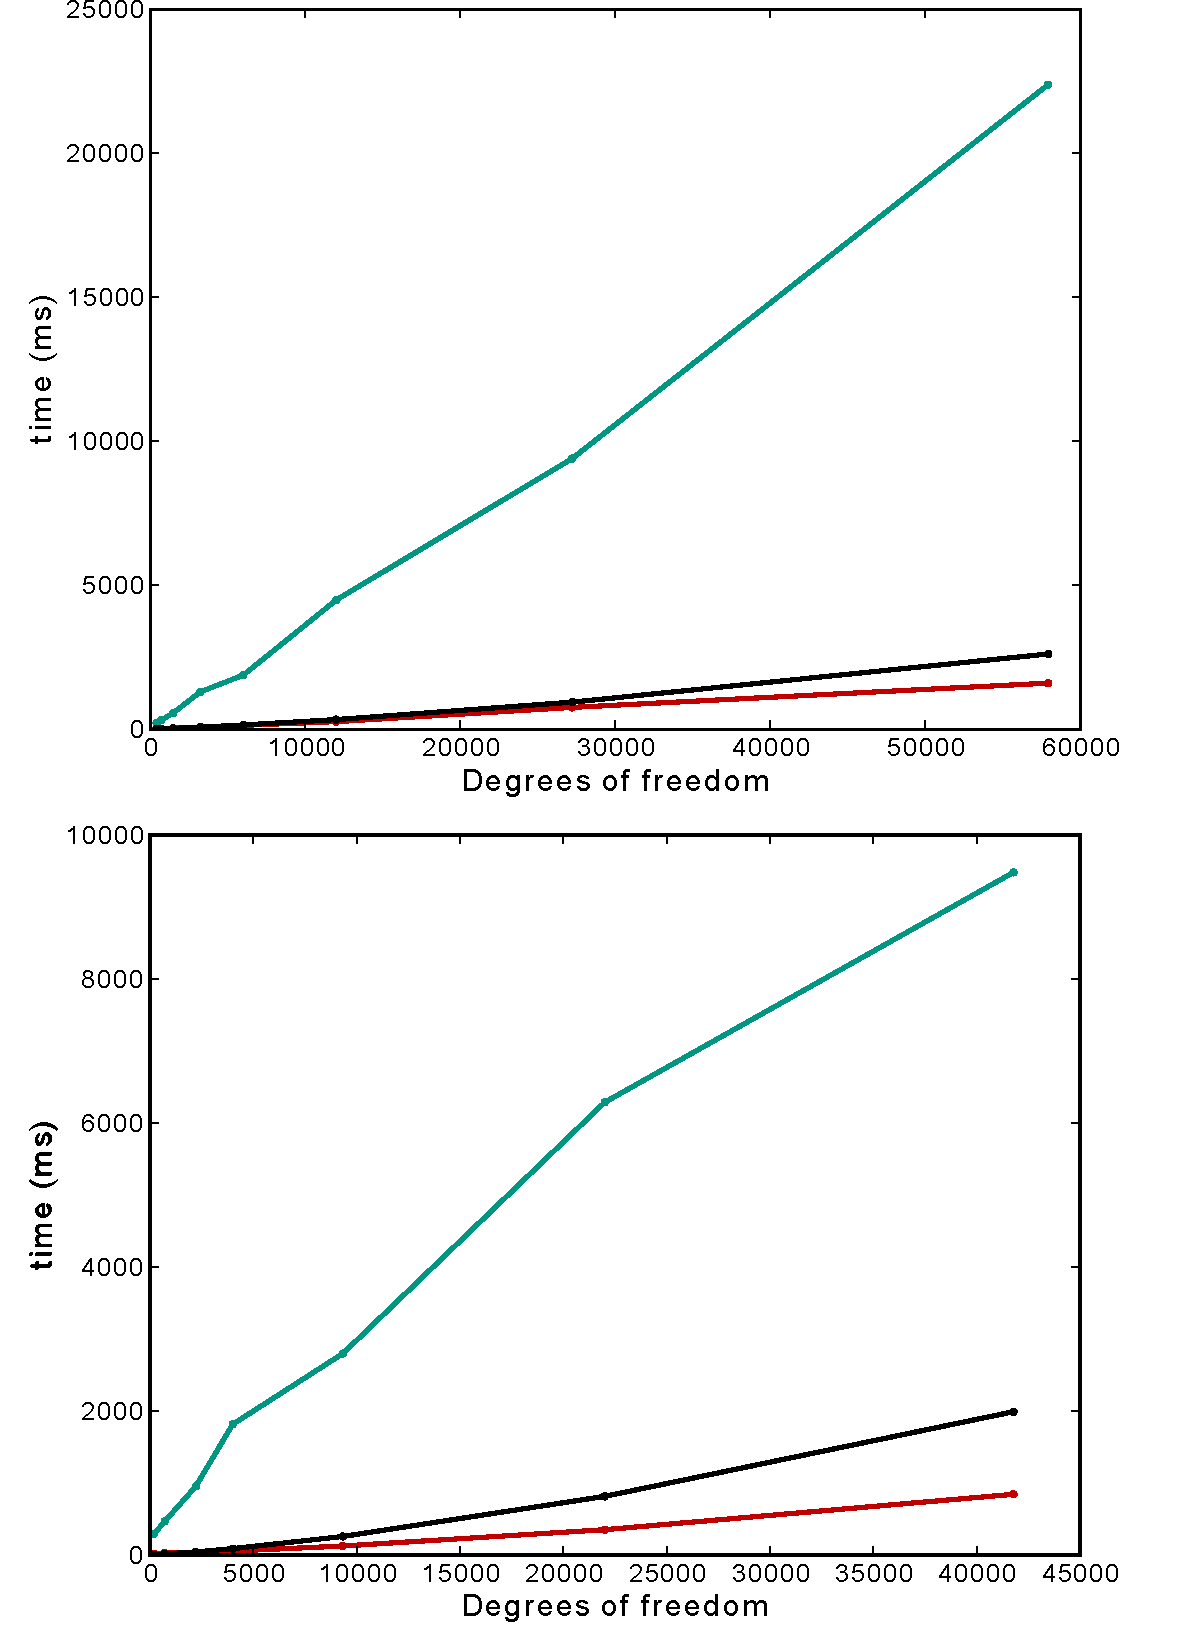
\includegraphics[width=0.92\textwidth]{Figures/PerformanceComparisonFinalGPUPardiso.pdf}     
\caption{Solution times for the tet4 beam (top) and the tet10 beam (bottom). Timings for the CPU based FSAI(2)-PCG solver (green) and the GPU variant of the algorithm (red) are listed as well as the total solve time for the direct Pardiso solver (black). }
\label{PerformanceComparisonFinalGPUPardiso}
\end{figure}

\subsection{GPU based multigrid solver}
We apply the proposed GPU based multigrid (MG) scheme to the beam model under gravitational load that was presented in the previous section. We analyze a discretization with 100120 tet4 elements (57915 DOF) and a tet10-based model with 8990 elements (41781 DOF). A residual of $0.01$ is used as the stopping criterion for the CG scheme. Furthermore, a grid hierarchy of 3 levels is used: For the tet4 beam the meshes consist of 100120, 8990 and 1810 elements, wheres the tet10 hierarchy is made up of meshes with 8990, 712 and 97 elements. For all MG computations, we use one iteration with a FSAI(2) scheme for smoothing purposes. The inner PCG solver uses an FSAI(2) preconditioner with rotation warping and a residual threshold of $0.01$.

The results of the computations are listed in Table \ref{TimingsMGComputations}. For comparison purposes, we also list the corresponding timings for the direct single-core Pardiso solver and the FSAI-preconditioned GPU-CG scheme that was extensively discussed in the previous section. As the nodal forces have to be computed on all levels in order to update the elemental stiffness matrices with the current rotation, their computation time ($t_{force}$) is slightly higher for the MG solver. However, the additional overhead stays well below $20\%$ for all scenarios. It is also apparent that the multigrid scheme is a very efficient preconditioner as the CG scheme only needs a few iterations to convergence. In contrast, the FSAI-PCG scheme needs an average of 115 (tet4) and 80 (tet10) iterations. In case of the CPU variant of the MG method, the largest amount of time is spent in the smoother (179 ms per time step for the tet4 model and 116 ms for the tet10 model). This component of the algorithm can be significantly accelerated by using GPU hardware (up to 9x for the tet4 model). In contrast, the acceleration of the inner PCG solve is not as pronounced. This is due to the low size of the inner problems, which do not utilize the full computational power of the GPU.

Overall it can be seen that the proposed GPU-based multigrid scheme is a very efficient solver. For the linear tetrahedral mesh, it achieves a speed-up of nearly 10x in comparison with the direct solver (5x in comparison with the CPU-PCG approach). For the quadratic tetrahedral discretization, this difference is even more pronounced: Here, a speed-up of more than 15x is obtained in comparison with the direct solver.


\begin{table*}
	\centering
		\begin{tabular}{cccccccccc}
				\hline & Solver &   $t_{force}$ & $t_{sm}$& $t_{in}$ & $t_{pre}$ & $t_{cg}$ & $n_{cg}$ & $t_{solve}$ & $t_{tot}$ \\\hline 
				 \parbox[t]{0.5mm}{\multirow{3}{*}{\rotatebox[origin=c]{90}{tet4}}}&Pardiso &  408&  & & & & & 2712& 3120 \\
				& GPU-PCG &  147& & & 5& 5 & 115 & 1314 & 1461\\
				&CPU-MG &  477 & 179 & 17&274&48&3&979&1476 \\
				&GPU-MG &  149 & 20 & 18 &54&5&3& 178&327 \\
				\hline
				 \parbox[t]{0.5mm}{\multirow{3}{*}{\rotatebox[origin=c]{90}{tet10}}}&Pardiso &  621& & & & & & 2001&2622 \\
				&GPU-PCG &  71& & & 5&2&80&574&645 \\
				&CPU-MG &  690&116&7&154&15&2&386&1076 \\
				&GPU-MG &  88&22&6&35&2&2 &84&172 \\
		\end{tabular}
	\caption{Computation times in ms for nodal force computation $t_{force}$, application time for preconditioner per CG step $t_{precond}$ (for MG solvers the computation times for the smoothing operator $t_{sm}$ and the inner solve $t_{in}$ are listed as well) and for one pure CG step $t_{cg}$. Additional columns list the number of CG steps $n_{cg}$, the total linear solver time $t_{solve}$ and the total computation time $t_{tot}$ per time step in ms.}
	\label{TimingsMGComputations}
\end{table*}

\section{Discussion}

In the previous chapter we have demonstrated that quadratic tetrahedral discretizations severely outperform linear tetrahedral meshes in terms of accuracy per number of degrees of freedom. Due to volume locking, the linear tetrahedral mesh needs more than a magnitude more (up to 40x) DOF in order to achieve the same accuracy as a tet10 mesh. In this chapter, a novel mapping scheme for embedding high resolution surface models into low-resolution higher order computational meshes was proposed. The mapping is constructed using a non-linear optimization algorithm whose complexity scales linearly with the number of vertices in the surface model and is nearly independent of the number of elements in the computational model.

The main contribution of this chapter is a fast GPU-based solver for quadratic corotated FE. Based on the novel mapping scheme for higher order isoparametric meshes, a novel multigrid approach for non-conforming, unstructured grids was presented. By using a novel FSAI-preconditioned CG solver as the coarse problem solver and employing a highly parallel smoothing scheme, the developed MG solver can be efficiently implemented on the GPU. The MG scheme significantly outperforms the direct Pardiso solver as well as the state-of-the-art Jacobi-preconditioned GPU-CG solver by more than an order of magnitude. It allows to simulate a high resolution, 8990 tet10 elements (41781 DOF) problem at nearly 6 time steps per second. As we will see in the upcoming chapter, this model size definitely provides sufficient accuracy in order to be used in a soft tissue registration scheme.
 


%
%\begin{table*}
	%\centering
		%\begin{tabular}{ccccccccccc}
				%\hline & Solver &  DOF &  $t_{force}$ & $t_{sm}$& $t_{in}$ & $t_{pre}$ & $t_{cg}$ & $n_{cg}$ & $t_{solve}$ & $t_{tot}$ \\\hline 
				 %\parbox[t]{2mm}{\multirow{3}{*}{\rotatebox[origin=c]{90}{tet4}}}&Pardiso & 57915 & 408&  & & & & & 2712& 3120 \\
				%& GPU-PCG & 57915 & 147.1& & & 4.79& 9.58 & 115.29 & 1836.57 & 1984\\
				%&CPU-MG & 57915 & 477.09 & 178.56 & 16.98 &274.33&47.56&3.04&978.55&1475.62 \\
				%&GPU-MG & 57915 & 148.5 & 20 & 18.26 &53.64&5.05&3.04& 178.42&326.92 \\
				%\hline
				 %\parbox[t]{2mm}{\multirow{3}{*}{\rotatebox[origin=c]{90}{tet10}}}&Pardiso & 41781 & 621.07& & & & & & 2000.98&2622.05 \\
				%&CPU-PCG & 41781 & 70.86& & & 5.23&4.71&79.87&819.47&890.33 \\
				%&CPU-MG & 41781 & 689.98&116.1&6.78&154.29&14.99&2.28&385.96&1075.94 \\
				%&GPU-MG & 41781 & 87.82&21.92&6.17&35.17&1.64&2.28 &83.93&171.75 \\
		%\end{tabular}
	%\caption{Computations times in ms for nodal force computation $t_{force}$, computation of nodal rotations $t_{nrot}$, application time for preconditioner per CG step $t_{precond}$ and for one pure CG step $t_{cg}$. Additional columns list the number of CG steps $n_{cg}$, the total linear solver time $t_{solve}$ and the total computation time $t_{tot}$ per time step in ms.}
	%\label{tab:Timings}
%\end{table*}




%Computation times for different algorithmic setups for the beam under gravity load are given in Table. \ref{tab:Timings}. All timings are averaged over 20 time steps. It can be seen that the number of CG  iterations $n_{cg}$ can be reduced by nearly an order of magnitude through the use of the FSAI preconditioner. The reduction is slightly more pronounced for the FSAI(3) preconditioned tet4 problems than for the FSAI(2) preconditioned tet10SR problems. However, the PCG approach requires the computation of the nodal rotations per time step ($t_{nrot}$) as well as the application of the preconditioner ($t_{precond}$) and its warping per CG step. While the additional nodal rotation warping is negligible and dominated by the kernel launch overhead (max. 0.08ms for all problems), the additional two SpMV multiplications needed for the preconditioner application substantially increase the computation time per CG step. Because of this increased computational complexity the speed-up related to the total linear solver time $t_{solve}$ for the PCG is about $5x$ for the tet4 problems and $3.5x$ for the tet10SR problems. It is important to point out that a residual of $1e-3$ was used as the stopping criterion for the CG iterations. A larger residual can be used in order to reduce the number of iterations for applications that don't require physical accuracy. However, there a minimal iteration count is required in order to maintain a stable simulation. It is also important to note that the reduction factor achieved through the use of a preconditioner remains approximately regardless of the enforced residual. For completeness, we list the time for the computation of the nodal forces $t_{force}$. These are dominated by the polar decomposition and the ensuing rotation of the element matrices. It is apparent that this step needs only little time in comparison with the linear system solve (especially for larger meshes). 
%
%\begin{table*}
	%\centering
		%\begin{tabular}{lcccccccccc}
				%\hline Model & Tetrahedra & DOF & Solver & $t_{force}$ & $t_{nrot}$  & $t_{precond}$ & $t_{cg}$ & $n_{cg}$ & $t_{solve}$ & $t_{tot}$ \\\hline 
				%Beam tet4 low & 4610 & 3222 & CPU CG & 16.91 & 0 &  0 & 2.33 & 798 & 1859 & 1876 \\
				%Beam tet4 low & 4610 & 3222 & CPU FSAI(3)-PCG & 16.44 & 2.6 &  1.72 & 2.39 &50 & 207.5  & 224 \\
				%Beam tet10SR low & 712 & 4002 & CPU CG & 61.15 & 0 &  0 & 2.16 & 1069 & 2309 & 2370 \\
				%Beam tet10SR low & 712 & 4002 & CPU FSAI(2)-PCG & 60.9 & 1.94 &  2.36 & 2.01 & 80 & 350 & 411 \\
				%Beam tet4 high & 19128 & 11982 & CPU CG & 69.58 & 0 &  0 & 11.21 & 1269 & 14225& 14295 \\
				%Beam tet4 high & 19128 & 11982 & CPU FSAI(3)-PCG & 69.57 & 12.23 &  8.25 & 10.65 & 147 & 2787 & 2865 \\
				%Beam tet10SR high & 4610 & 22002 & CPU CG & 378.3 & 0 &  0 & 12.99 & 1831 & 23785 & 24163 \\
				%Beam tet10SR high & 4610 & 22002 & CPU FSAI(2)-PCG & 378.8 & 11.7 &  16.52 & 12.56 & 242 & 7059 & 7436 \\
				%\hline
				%Beam tet4 low & 4610 & 3222 & GPU FSAI(3)-PCG & 4.72  & 3.38 & 0.31 &  0.67 & 50 & 49 & 53.72 \\
				%Beam tet10SR low & 712 & 4002 & GPU FSAI(2)-PCG & 16.54  & 2.25 & 2.84 &  0.82 & 80 & 90 & 107 \\
				%Beam tet4 high & 19128 & 11982 & GPU FSAI(3)-PCG & 20.7 & 4.5 &  1.03 & 1.51 & 147 & 373 & 394 \\
				%Beam tet10SR high & 4610 & 22002 & GPU FSAI(2)-PCG & 24.83 & 4.15 &  2.36 & 2.66 & 242 & 1215 & 1240 \\
		%\end{tabular}
	%\caption{Computations times in ms for nodal force computation $t_{force}$, computation of nodal rotations $t_{nrot}$, application time for preconditioner per CG step $t_{precond}$ and for one pure CG step $t_{cg}$. Additional columns list the number of CG steps $n_{cg}$, the total linear solver time $t_{solve}$ and the total computation time $t_{tot}$ per time step in ms.}
	%\label{tab:Timings}
%\end{table*}
%
%Table \ref{tab:Timings} also shows that the GPU implementation of the PCG algorithm is approx. 6x (tet10SR) to 7x (tet4) faster than the CPU implementation. The slightly higher speed-up for linear elements can be attributed to the fact that some parallelization strategies (e.g. coloring) depend on the number of elements rather than the number of nodes. In this context, the quadratic mesh sizes of 712 and 4610 elements respectively might even be too small to use the GPU to full capacity. Although our GPU code for nodal force computation isn't fully optimized it is apparent that for larger problems (tet10SR, 22002 DOF problem), this part of the FE simulation can greatly benefit from a GPU implementation.

%
%\section{Discussion}
%
%We have presented a detailed numerical and graphical comparison between linear and quadratic corotated finite elements for deformable body simulation. It is apparent that linear elements often need more than order of magnitude more DOFs to achieve the same accuracy than quadratic elements. This is not only true for high-resolution meshes, but also for small model sizes. In order to leverage the power of higher order isoparametric elements, we proposed a novel mapping scheme for embedding highly detailed triangular surface meshes to the computational grid. This mapping preserves local shape features and causes only negligible overhead during the simulation. It is constructed
%by representing each surface vertex in terms of points on the computational mesh and its distance to the FE mesh in normal direction. We proposed a recursive mapping scheme based on non-linear optimization to robustly construct this representation for curved isoparametric higher order FE meshes. The numerical complexity of the mapping scheme is linear in the number of surface nodes and independent of the size of the coarse computational mesh. 
%
%The numerical results show that the solution time of the FE algorithm is dominated by the linear solver. In order to speed up this component we presented an efficient GPU-based PCG algorithm. This is achieved by using an explicit, pre-computed preconditioner that is adapted for each time step using nodal rotation warping. Using the GPU-based approach, the complete FE simulation runs between $20x$ (quadratic elements) and $36x$ (linear elements) faster than a CPU based pure CG scheme. As the computational time for quadratic meshes is comparable to linear meshes with the same number of DOF, it is apparent that a combination of quadratic elements with the GPU based solver can yield speed-ups of more than two order of magnitude compared to a co-rotational method with linear shape functions on the CPU. 
%
%The main drawback of the method is the setup time for the FSAI preconditioner. If a single core implementation is used, the building of the preconditioner can take hours for larger meshes. This disadvantage can be alleviated by building the preconditioner offline in a precomputation step and just loading it from disk at the beginning of each simulation. Furthermore, recent work in this area shows that GPU implementation of the building phase can drastically reduce the setup time \cite{Dehnavi2012}.
%
%We would like to point out that the mapping scheme is neither restricted to quadratic elements nor to tetrahedral elements. The approach can be used to map highly detailed surface mesh to shell or volume meshes of arbitrary order and element type. The mapping approach might thus be able to facilitate the use of higher order elements for real-time simulations.   
%
%It is well known that multigrid based techniques constitute very efficient solving scheme for elastic problems \cite{Zhu2010}. Since these schemes scale linearly with the mesh size, they are especially useful for high resolution meshes. However, the implementation of multigrid schemes on the GPU for unstructured grids is challenging. We would like to emphasize that the contributions of this paper provides the two essential blocks for a GPU-based multigrid scheme for unstructured higher order FE meshes. Not only can the proposed mapping technique be used to transfer displacements between the grids at different resolution, but the FSAI preconditioner can also be used as a smoother in a multigrid scheme \cite{Heuveline2012}. Thanks to the rotation warping technique, FSAI based smoothing can be used in real-time simulations.



  



\begin{appendix}
%\input{AppendixA}

%\chapter{Appendix}

\chapter{Additional remarks on elasticity theory and FE methods} 

\section{Basics of vector analysis} 

\subsection{Divergence theorem}
\label{ADivergenceTheorem}
For any smooth vector field $\mv(\mbx)$ and any smooth tensor field $\mathbf{A}(\mbx)$ that are defined on a compact region $\Omega$ which is enclosed by the smooth, closed surface $\partial \Omega$ we have
\begin{eqnarray}
\int _{\partial \Omega} \mv \cdot \mn \mdA = \int _{\Omega} \mdiv \mv \mdV \qquad \textnormal{or} \qquad \int _{\partial \Omega} v_i n_i \mdA = \int _{\Omega} \frac{\partial v_i}{\partial x_i} \mdV
\end{eqnarray}

\begin{eqnarray}
\int _{\partial \Omega} \mathbf{A}  \mn \mdA = \int _{\Omega} \mdiv \mathbf{A} \mdV \qquad \textnormal{or} \qquad \int _{\partial \Omega} A_{ij} n_j \mdA = \int _{\Omega} \frac{\partial A_{ij}}{\partial x_j} \mdV
\end{eqnarray}

\subsection{Product differentiation rules for tensors}
\label{AProductRule}
For any smooth vector field $\mv(\mbx)$ and any smooth tensor field $\mathbf{A}(\mbx)$ we have

\begin{eqnarray}
\mdiv(\mathbf{A}^T \mv) = \mdiv(\mathbf{A}) \cdot \mv + \mdiv(\mathbf{A}) : \mgrad( \mv)
\end{eqnarray}

\section{Work conjugancy of $\mbS$ and $\dot{\mbE}$} 
\label{WorkConjugancySE}

It has already been shown in section (\ref{SectionMechanicalEnergyInElasticBodies}) that the first Piola-Kirchhoff stress tensor $\mbP$ is work conjugated to the material time derivative of the deformation gradient $\mbF$. It is quickly shown that the material time derivative of the Cauchy-Green strain tensor $\mbC$
\begin{alignat}{1}
\dot \mbC = \mddt \left( \mbF ^T \mbF \right) = \mbdotF ^T \mbF + \mbF ^T \mbdotF
\end{alignat}
related to the material time derivative of the Green-Lagrange strain tensor by
\begin{alignat}{1}
\dot \mbE = \mddt \frac{1}{2} \left( \mbF ^T \mbF  - \mbI\right) = \frac{1}{2} \left( \mbdotF ^T \mbF + \mbF ^T \mbdotF \right) = \frac{1}{2} \dot \mbC.
\end{alignat}

Based on the results of section \ref{SectionMechanicalEnergyInElasticBodies} (work conjugancy of $\mbP$ and $\mbdotF$), we can thus derive 
\begin{alignat}{1}
\mbP : \mbdotF  &= \mtr(\mbP ^T \mbdotF) = \mtr(\mbdotF ^T \mbP) = \mtr(\mbdotF ^T \mbF \underbrace{ \mbF ^{-1} \mbP}_{\mbS}) \\
&= \mtr(\mbS \mbdotF^T \mbF) =  \mtr(\mbS \mbF \mbdotF^T ) = \mtr(\mbS \frac{1}{2}(\mbdotF^T \mbF +  \mbF \mbdotF^T )) \\
&= \frac{1}{2} \mbS: \dot{\mbC} = \mbS: \dot{\mbE}
\end{alignat}

\section{The Saint Venant-Kirchhoff model} 
\label{ASVKModel}

The elastic energy functional for Saint-Venant Kirchhoff model is defined by
 \begin{equation}
 \mPsi  (\mbE )  = \frac{\lambda}{2} (\mtr \mbE)^2 + \mu \mtr (\mbE^2).
\end{equation}

In order to express the relation 
 \begin{equation}
 \mbS (\mbE) = \frac{ \partial \mPsi  (\mbE )}{\partial \mbE},
\end{equation}

we note the partial derivatives 

 \begin{equation}
\frac{\partial \mtr (\mbE)}{\partial \mbE} = \frac{1}{\partial E_{ij}} \sum_{k=1} ^3 E_{kk} = \delta_{ij} = \mbI
\end{equation}

and

 \begin{equation}
 \mbS (\partial \mbE) = \frac{\partial \mtr (\mbE^2)}{\partial \mbE} = \frac{1}{\partial E_{ij}} \sum_{k,l=1} ^3 E_{kl} E_{kl} = 2 E_{ij} = 2 \mbE.
\end{equation}

Thus, we obtain

 \begin{equation}
\frac{ \partial \mPsi  (\mbE )}{\partial \mbE} = \frac{\lambda}{2} \frac{ \partial \left( (\mtr \mbE)^2 \right)}{\partial \mbE } + \mu \frac{ \partial \left( \mtr (\mbE^2) \right) }{\partial \mbE} = \lambda \mtr{\mbE} \mbI + 2 \mu \mbE.
\end{equation}

\section{Polynomial shape functions for selected elements} 
\label{AShapeFunctions}

\begin{figure}
   \centering   
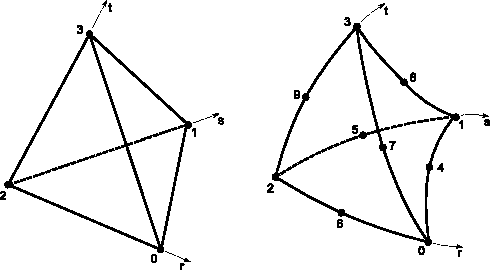
\includegraphics[width=8.5cm]{Figures/Tet4and10.pdf}
\caption{Linear tetrahedron with 4 nodes (tet4) and quadratic tetrahedron with 10 nodes (tet10)}
\label{TetraAppendix}
\end{figure}

\subsection{Nodal shape functions in local (curvilinear) coordinates}
Linear 4-node tetrahedron (node numbering as shown in Fig. \ref{TetraAppendix}):
\begin{alignat}{1}
N_0(r,s,t) &= r\\ 
N_2(r,s,t) &= s\\
N_3(r,s,t) &= 1-r-s-t\\
N_4(r,s,t) &= t\\
\end{alignat}

Quadratic 10-node tetrahedron (node numbering as shown in Fig. \ref{TetraAppendix}):
\begin{alignat}{1}
N_0(r,s,t) &= (2r-1)r\\ 
N_1(r,s,t) &= (2s-1)s\\
N_2(r,s,t) &= (2 (1-r-s-t) -1)(1-r-s-t)\\
N_3(r,s,t) &= (2t-1)t\\
N_4(r,s,t) &= 4rs\\
N_5(r,s,t) &= 4(1-r-s-t)s\\
N_6(r,s,t) &= 4(1-r-s-t)r\\
N_7(r,s,t) &= 4st\\
N_8(r,s,t) &= 4rt\\
N_9(r,s,t) &= 4(1-r-s-t)t\\
\end{alignat}

\subsection{Nodal shape functions in global coordinates}

The standard triangle [(1,0,0) (0,1,0) (0,0,0) (0,0,1)] is mapped to the global coordinate system using the shape functions (isometric elements). If $\mathbf X_k$ denotes the initial position of the k-th node of the n-node tetrahedron, we define the function $\xi(\mathbf r)$ that maps the local coordinates $\mathbf r = (r,s,t)$ to the global coordinates $\mbX = (X_1, X_2,X_3)$:
\begin{equation}
\xi (\mathbf {r}) = \mbX (\mathbf{ r}) = \mbX (r,s,t) = \sum_{k=0} ^n \mbX _k N_k(r,s,t)
\end{equation}

The global derivatives of the shape functions are
\begin{equation}
\frac{\partial N_I(\mbx)}{\partial \mbX} = \mathbf J^{-1} \frac{\partial N_I(\mbx)}{\partial \mathbf r}
\end{equation}

where $\mathbf J$ is the jacobian
\begin{equation}
\mathbf J = \nabla \xi = \left(
\begin{array}{ccc}
\frac{\partial X_1}{\partial r} & \frac{\partial X_2}{\partial r} & \frac{\partial X_3}{\partial r}\\
\frac{\partial X_1}{\partial s} & \frac{\partial X_2}{\partial s} & \frac{\partial X_3}{\partial s}\\
\frac{\partial X_1}{\partial t} & \frac{\partial X_2}{\partial t} & \frac{\partial X_3}{\partial t}
\end{array}
\right)
\end{equation}




\section{Internal nodal forces and the stiffness matrix for linear elasticity} \label{ANodalForces}

As detailed in section \ref{SectionMatrixFormulation}, the internal nodal forces are given by

\begin{eqnarray}
\mfint = \mfintThree = \mIntRConf \mfintDens \mdVZero = \sum_{e} \mIntREl \mfintDens \mdVZero = \mIntRConf \msigma_{ik}  \left( \nabla \mtfTwo \right)_{kI} \mdVZero.
\end{eqnarray}

By noting that the gradient of the displacement vector reads
\begin{eqnarray}
\nabla \mbu = \nabla (\mcu _I \mtf ) =  \mcu _I \nabla \mtf = \mcu _{iI} \left( \nabla \mtfTwo \right)_{kI},
\end{eqnarray}

we can express its the derivative with respect to the nodal displacements through
\begin{eqnarray}
\frac{\partial}{\partial \mcu _{jJ}} \left( \nabla \mcu \right)_{ik}  = \frac{\partial}{\partial \mcu _{jJ}} \left( \mcu _{iI} \left( \nabla \mtfTwo \right)_{kI} \right) = \delta _{ij} (\nabla \mtfTwo_{kJ}).
\end{eqnarray}


The derivative of the Cauchy strain with respect to the nodal displacements can thus be derived as
\begin{eqnarray}
\frac{\partial \meps _{ik}}{\partial \mcu _{jJ}} &=& \frac{1}{2} \frac{\partial}{\partial \mcu _{jJ}} \left( \nabla \mbu + (\nabla \mbu )^T \right) \notag \\
&=& \frac{1}{2} \frac{\partial}{\partial \mcu _{jJ}} \left(  \mcu _{iI} \left( \nabla \mtfTwo \right)_{kI}  + \mcu _{kI} \left( \nabla \mtfTwo \right)_{iI} \right) \notag \\
&=& \frac{1}{2}  \left( \delta _{ij} (\nabla \mtfTwo)_{kJ} + \delta _{kj} (\nabla \mtfTwo)_{iJ} \right).
\end{eqnarray}

Consequently, the derivation of the Cauchy stress follows as
\begin{eqnarray}
\frac{\partial \msigma _{ik}}{\partial \mcu _{jJ}} &=& 2\mu \frac{\partial \meps_{ik}}{\partial \mcu _{jJ}} + \lambda \delta _{ik} \frac{\partial \meps_{ll}}{\partial \mcu _{jJ}} \notag \\
&=& \mu \left( \delta _{ij} (\nabla \mtfTwo)_{kJ} + \delta _{kj} (\nabla \mtfTwo)_{iJ} \right) + \frac{\lambda}{2}  \delta _{ik} \left( \delta _{lj} (\nabla \mtfTwo)_{lJ} + \delta _{lj} (\nabla \mtfTwo)_{lJ} \right) \notag \\
&=& \mu \left( \delta _{ij} (\nabla \mtfTwo)_{kJ} + \delta _{kj} (\nabla \mtfTwo)_{iJ} \right) + \frac{\lambda}{2} 2 \delta _{ik} (\nabla \mtfTwo)_{jJ} \notag \\
&=& \mu \delta _{ij} (\nabla \mtfTwo)_{kJ} + \mu \delta _{kj} (\nabla \mtfTwo)_{iJ}  + \lambda \delta _{ik} (\nabla \mtfTwo)_{jJ} 
\end{eqnarray}

and the derivative of the internal force density can be expressed as
\begin{eqnarray}
\frac{\partial \mfintDens}{\partial \mcu _{jJ}} &=& \frac{\partial}{\partial \mcu _{jJ}} \left( \msigma_{ik}  \left( \nabla \mtfTwo \right)_{kI} \right) \mdVZero \notag \\
&=&  \frac{\partial \msigma_{ik}}{\partial \mcu _{jJ}} \left( \nabla \mtfTwo \right)_{kI}  \notag \\
&=& \left( \mu \delta _{ij} (\nabla \mtfTwo)_{kJ} + \mu \delta _{kj} (\nabla \mtfTwo)_{iJ}  + \lambda \delta _{ik} (\nabla \mtfTwo)_{jJ} \right) \left( \nabla \mtf \right)_{kI}  \notag \\
&=& \left( \mu \delta _{ij} (\nabla \mtfTwo)_{kJ} + \mu \delta _{kj} (\nabla \mtfTwo)_{iJ}  + \lambda \delta _{ik} (\nabla \mtfTwo)_{jJ} \right) \left( \nabla \mtf \right)_{kI}  \notag \\
&=&   \mu \delta _{ij} (\nabla \mtfTwo)_{kJ} \left( \nabla \mtf \right)_{kI} + \mu (\nabla \mtfTwo)_{iJ} \left( \nabla \mtf \right)_{jI} \notag \\
& & + \lambda  (\nabla \mtfTwo)_{jJ} \left( \nabla \mtf \right)_{iI}.
\end{eqnarray}

This yields the stiffness matrix
\begin{eqnarray}
\frac{\partial \mfintThree}{\partial \mcu _{jJ}} = \mIntRConf \frac{\partial \mfintDens}{\partial \mcu _{jJ}} \mdVZero = \sum_{e} \mIntREl \frac{\partial \mfintDens}{\partial \mcu _{jJ}} \mdVZero = \sum_{e} \mathbf{K}^e =  \msmat.
\end{eqnarray}

\section{Internal nodal forces and the stiffness matrix for corotated elasticity} \label{ACorotNodalForces}

The polar decomposition of deformation gradient (see section \ref{SectionPolarDecomposition})

\begin{eqnarray}
\mathbf F = \mathbf R \mathbf U
\end{eqnarray}

is used to define the stretch measure
\begin{eqnarray}
\mathbf U = \mathbf {R} ^T \mathbf F.
\end{eqnarray}

We express the displacement gradient through the nodal positions 
\begin{eqnarray}
\nabla \mbu = \mbF - \mbI = \nabla ( \mcx_J  \mbf ) =  \mcx_J  \nabla  \mbf - \mbI
\end{eqnarray}

in order to relate the Cauchy strain to the nodal positions:
\begin{eqnarray}
\meps &=& \frac{1}{2} \left( (\mbF - \mbI ) + (\mbF - \mbI  )^T \right)  = \frac{1}{2} \left( (\mcx_J  \nabla  \mbf - \mbI)+ (\mcx_J  \nabla  \mbf - \mbI )^T \right)  \notag \\
&=& \frac{1}{2} \left( \mcx_{iJ} (\nabla \mtfn)_{jJ} +  \mcx_{jJ} (\nabla \mtfn)_{iJ} \right) - \mbI.
\end{eqnarray}

For corotated elasticity, the deformation gradient is replaced by the stretch measure
\begin{equation}
\mSt = \mrot^T \nabla \mbF = R_{ki} \mcx_{kJ}  (\nabla \mtfn)_{jJ}.
\end{equation}



Consequently, the corotated Cauchy strain reads
\begin{eqnarray}
\meps ^{CR} &=& \meps_{ij} ^{CR} = \frac{1}{2} \left( \mrot^T \mcx_J \nabla \mbf +  (\mrot^T \mcx_J \nabla \mbf)^T \right) - \mbI
\end{eqnarray}

and the corotated stress is derived to
\begin{eqnarray}
\msigma_{ij} ^{CR} &=& 2\mu \meps^{CR}_{ij} + \lambda \delta _{ij} \meps^{CR}_{ll} \notag.
\end{eqnarray}

We note that the internal nodal forces can be written in terms of the variation of nodal position 
\begin{eqnarray}
D_{\delta \mcu} \meFunc (\mbu _h) _{int} &=& \mIntRConf \msigma : \delta \meps  \mdVZero =  \mIntRConf \msigma : \frac{1}{2} \left( \delta \nabla \mbu + (\delta \nabla \mbu)^T \right)  \mdVZero \notag\\
&=&  \mIntRConf \msigma :  \delta \nabla \mbu  \mdVZero = \mIntRConf \msigma : \left( \delta \mcu_I \nabla \mtf \right) \mdVZero \notag\\
&=& \mIntRConf \msigma : \left( \delta \mcx_I \nabla \mtf \right) \mdVZero
\end{eqnarray}

in order to derive the corotated nodal forces
\begin{eqnarray}
D_{\delta \mcu} \meFunc (\mbu _h) _{int} &=& \mIntRConf \msigma : \left( \mrot^T \delta \mcx_I \nabla \mtf \right) \mdVZero = \mIntRConf (\mrot \msigma) : \left(  \delta \mcx_I \nabla \mtf \right) \mdVZero \notag \\
&=& \delta \mcx_{iI} \mIntRConf \mrot_{im} \msigma_{mk}  (\nabla \mtfTwo)_{kI} \mdVZero = \delta \mcx_{iI} \mIntRConf \mfintDensCR \mdVZero  \notag \\
&=& \delta \mcx_{iI} \mfintThreeCR= \delta \mcx_I \mfintTwoCR
\end{eqnarray}

with
\begin{eqnarray}
\mfintDensCR =   \mIntRConf \mrot_{im} \msigma^{CR}_{mk}  (\nabla \mtfTwo)_{kI} \mdVZero.
\end{eqnarray}

In order to formulate the corotated stiffness matrix, we first compute the derivate of the corotated Cauchy strain with respect to the nodal positions:
\begin{eqnarray}
\frac{\partial \meps _{mk}}{\partial \mcx _{jJ}} &=& \frac{1}{2} \frac{\partial}{\partial \mcx _{jJ}} \left(R_{nm} F_{nk} + F_{nm} R_{nk}  \right) - \mbI \notag \\
&=& \frac{1}{2} \frac{\partial}{\partial \mcx _{jJ}} \left(R_{nm} \mcx_{nI} \left( \nabla \mtfTwo \right)_{kI}  + \mcx_{nI} \left( \nabla \mtfTwo \right)_{mI} R_{nk}  \right) \notag \\
&=& \frac{1}{2}  \left( \delta_{nj} R_{nm}  \left( \nabla \mtfTwo \right)_{kJ}  + \delta_{nj}\left( \nabla \mtfTwo \right)_{mJ} R_{nk}  \right) 
\end{eqnarray}

In a similar fashion as in the linear elastic case we derive
\begin{alignat}{1}
& \frac{\partial \msigma^{CR} _{mk}}{\partial \mcx _{jJ}} = 2\mu \frac{\partial \meps^{CR}_{mk}}{\partial \mcx _{jJ}} + \lambda \delta _{mk} \frac{\partial \meps^{CR}_{ll}}{\partial \mcx _{jJ}} \notag \\
&= \mu \left(  \delta_{nj} R_{nm}  \left( \nabla \mtfTwo \right)_{kJ}  + \delta_{nj}\left( \nabla \mtfTwo \right)_{mJ} R_{nk}  \right) \notag \\
& + \frac{\lambda}{2}  \delta _{mk} \left( \delta_{nj} R_{nl}  \left( \nabla \mtfTwo \right)_{lJ}  + \delta_{nj}\left( \nabla \mtfTwo \right)_{lJ} R_{nl}  \right)  \notag \\
&= \mu \left(  \delta_{nj} R_{nm}  \left( \nabla \mtfTwo \right)_{kJ}  + \delta_{nj}\left( \nabla \mtfTwo \right)_{mJ} R_{nk}  \right) + \lambda  \delta _{mk}  \delta_{nj} R_{nl}  \left( \nabla \mtfTwo \right)_{lJ}
\end{alignat}

and express the corotated force density through
\begin{eqnarray}
& &\frac{\partial \mfintDens}{\partial \mcx _{jJ}} = \frac{\partial}{\partial \mcx _{jJ}}  \mrot_{im} \msigma^{CR}_{mk}   \left(  \nabla \mtfTwo \right)_{kI} = \mrot_{im} \frac{\partial \msigma^{CR}_{mk}}{\partial \mcx _{jJ}}    \left(  \nabla \mtfTwo \right)_{kI} \notag \\
&=&   \mrot_{im} \left( \mu \left(  \delta_{nj} R_{nm}  \left( \nabla \mtfTwo \right)_{kJ}  + \delta_{nj}\left( \nabla \mtfTwo \right)_{mJ} R_{nk}  \right) + \lambda  \delta _{mk}  \delta_{nj} R_{nl}  \left( \nabla \mtfTwo \right)_{lJ}  \right)   \left(  \nabla \mtfTwo \right)_{kI}  \notag \\
&=& \mrot_{im}   \mu \left(  \delta_{nm} R_{jn}  \left( \nabla \mtfTwo \right)_{kJ} \left(  \nabla \mtfTwo \right)_{kI} + \left( \nabla \mtfTwo \right)_{mJ} R_{jk} \left(  \nabla \mtfTwo \right)_{kI} \right) \notag \\
& &+ \lambda    R_{jl}  \left( \nabla \mtfTwo \right)_{lJ} \left(  \nabla \mtfTwo \right)_{mI}   \notag \\
&=& \mrot_{im}   \mu \left(  \delta_{nm}   \left( \nabla \mtfTwo \right)_{kJ} \left(  \nabla \mtfTwo \right)_{kI} R_{jn} + \left( \nabla \mtfTwo \right)_{mJ}  \left(  \nabla \mtfTwo \right)_{nI} \right) R_{jn} \notag \\
& &+ \lambda     \left( \nabla \mtfTwo \right)_{nJ} \left(  \nabla \mtfTwo \right)_{mI}  R_{jn}  \notag \\
&=& \mrot_{im}   \left( \mu \left(  \delta_{nm}   \left( \nabla \mtfTwo \right)_{kJ} \left(  \nabla \mtfTwo \right)_{kI}  + \left( \nabla \mtfTwo \right)_{mJ}  \left(  \nabla \mtfTwo \right)_{nI} \right) + \lambda     \left( \nabla \mtfTwo \right)_{nJ} \left(  \nabla \mtfTwo \right)_{mI} \right) R_{jn}  \notag \\
&=& \mrot_{im}  \frac{\partial \hat{f}  ^{int}_{mI} }{\partial \mcx _{nJ}}   R_{jn} = \mathbf{R}  \frac{\partial \mfintTwoCR }{\partial \mcx _{J}}   \mathbf{R}^T .
\end{eqnarray}

The global corotated stiffness matrix is then given by
\begin{eqnarray}
\msmat ^{CR} =  \sum_{e} \mIntREl \frac{\partial \mfintDens}{\partial \mcx _{jJ}} \mdVZero = \sum_{e} \mIntREl  \mathbf{R}  \frac{\partial \mfintDensTwo }{\partial \mcx _{J}}   \mathbf{R}^T \mdVZero. 
\end{eqnarray}

%Similarly, we can derive the tangent stiffness for $\mthZero \mcx$:
%\begin{eqnarray}
%\mthZero \msmat_{IJ}  = \mthZero \msmat_{iIjJ}  =  \sum_{e} \mIntREl \frac{\partial \mfintDens}{\partial \mthZero \mcx  _{jJ}} \mdVZero  &=&  \sum_{e} \mIntREl  \mrot_{im}  \frac{\partial \hat{f}  ^{int}_{mI} }{\partial \mthZero \mcx  _{nJ}}  \mdVZero = \sum_{e} \mIntREl  \mathbf{R}  \frac{\partial \mfintDensTwo }{\partial \mthZero \mcx   _{J}}  \mdVZero  
%\end{eqnarray}
%
%Consequently the internal forces can be described as:
%\begin{eqnarray}
%\mfint_{I} = \msmat_{IJ}^{CR} \mcx  _{J} - \mthZero \msmat_{IJ}^{CR} \mthZero \mcx  _{J}
%\end{eqnarray}





\chapter{Glossary}





%\printglossaries
\setlength{\tabulinesep}{3pt}


    \begin{longtabu}{ R{2.4cm}  L{8cm} }
		$\mathbf A$ & arbitrary matrix (e.g. system matrix for linear system) \\
		$\mathcal{A}$ & additional DOF for sign enriched elements\\
		$\mBody$ & body (object) under analysis \\
		$\mbC$ & Cauchy-Green strain tensor \\
		$\mboC$ & modified (isochoric) Cauchy-Green strain tensor \\
		$\mdmat$ & damping matrix\\
		$\mbd$ & rate of deformation tensor \\
				$\mbdA , \mdA \mbn $& infinitesimal area element in current configuration \\
				$\mbdA_0 , \mdA_0 \mbN $& infinitesimal area element in reference configuration \\
				$\mdiv$ & divergence operator in current configuration \\
				$\mDiv$ & divergence operator in reference configuration \\
					$\mdV $& infinitesimal volume element in current configuration \\
		$\mdVZero $& infinitesimal volume element in reference configuration \\
		$\mbdx,\mdx_i $& line element in current configuration \\
		$\mbdX,\mdX_i$& line element in reference configuration \\
				$\mcdu$ & difference vector of nodal displacements \\
						$\mcdv$ & difference vector of nodal velocities \\
		$\mcdx$ & difference vector of nodal positions \\
		$\mdt$ & increment during time integration \\

		$\mbE$ & Green-Lagrange strain tensor \\
		$\mElemSetVert$ & set of elements in $\mMesh$ \\
		$\meps$ & infinitesimal strain tensor \\
		$\mfext$, $\mfextTwo$, $\mfextThree$ & vector of external nodal forces \\
		$\mfint$, $\mfintTwo$, $\mfintThree$ & vector of internal nodal forces \\
		
		$\mfintDens$ & internal force density \\	
		$\mfintCR$, $\mfintTwoCR$, $\mfintThreeCR$ & vector of corotated internal nodal forces \\
			$\mfintDensCR$ & internal force density \\		
		$\mbF $& deformation gradient tensor \\
		$\mbdotF $& time derivative of the deformation gradient tensor\\
		$\mboF$ & modified (isochoric) deformation gradient tensor \\
		$\mBCC$& boundary of the cut with zero Neumann (force) boundary conditions \\
		$\mBCN$& boundary with Dirichlet (displacement) boundary conditions \\
		$\mBCD$& boundary with Neumann (force) boundary conditions \\
		$\mrf$ & Cauchy-elastic response function\\ %G
		$\mgrad$ & gradient operator in current configuration\\
		$\mGrad$ & gradient operator in reference configuration\\		
		$\mbg$ & gravity acceleration vector \\		
		$\mrF$ & hyperelastic response function \\%H
		$\mH$ & Hamiltonian\\
		$\mbI $& identity matrix \\
		$\mbl$ & spatial velocity gradient \\
		$\msmat$ & stiffness matrix\\
		$\mK$ & kinetic energy \\
		$\mL$ & Lagrangian \\
		$\mmmat$ & mass matrix \\
		$\mMesh$ & finite element mesh \\		
		$\mbf, \mbffull$ & basis functions \\
		$\mtf, \mtfTwo_{iI}$ & test functions \\
		$\mbn$ & normal in current configuration \\
		$\mbN$ & normal in reference configuration \\
		$\mVert$& vertex in $\mSMesh$ \\
		$\liftOp$& lifting operator \\
		$\mRConf$ & region that is occupied by $\mBody$ in reference configuration \\ %Omega
		$\mCConf$ & region that is occupied by $\mBody$ in current configuration \\
		$\mbP$ & first Piola-Kirchhoff stress tensor \\
		$\mbp$ & point in $\mBody$ \\
		$\mPext$ & rate of external mechancial work (power input) \\
		$\meFunc$ & potential energy functional\\
		$\mPint$ & rate of internal mechanical work \\
		$\mPsi$ & internal elastic energy \\
		$\mrot$ & rotation matrix obtained from polar decomposition of $\mathbf F$\\
		$\rho$ & densitiy in current configuration \\
		$\rho_0$ & density in reference configuration \\
		$\mbS$ & second Piola-Kirchhoff stress tensor \\
		$\mSMesh$ & triangular surface mesh \\
		$\msigma$ & Cauchy stress tensor\\
		$\mt$ & traction vector in current configuration\\
		$\mbT$ & traction vector in reference configuration\\
		$\mTri$& element in $\mSMesh$\\
		$\mElem$ & element in $\mMesh$ \\
		$\mtr$ & trace operator \\
		$\mSt$ & stretch matrix obtained from polar decomposition of $\mathbf F$\\
     $\mbu,u_i $& displacement field \\
		$\mcu, \mcu_J, \mcu{jJ}$ & nodal displacement field \\
		$\mcv$& vector of nodal velocities \\
		$\mca$& vector of nodal accelerations \\
		$\mTFunc$ & variation of the displacement field\\
		$\mbw$ & rate of rotation tensor \\
		$\mv$ & velocity field	\\
		$\mdotv$ & acceleration field	\\
		$\mVertSetElem$ & set of vertices in $\mMesh$ \\		
		$\mBCSPD$ & space of functions that fulfill the Dirichlet boundary conditions on $\mBCD$\\
		$\mBCSPN$ & space of functions that fulfill the Neumann boundary conditions on $\mBCN$\\
		
		$\mwint$ & stress power per unit reference volume \\
		$\mbx,x_i$& positional field in the current configuration \\
		$\mbX,X_i $& positional field in the reference configuration \\
		$\mcx, \mcx_J, \mcx{jJ}$ & nodal positions \\
		
		
		
    \end{longtabu}







%elasticity basics

%

%
%\newcommand{\mgrad}{\ensuremath{ \textnormal{grad}}}
%\newcommand{\mGrad}{\ensuremath{ \textnormal{Grad}}}
%\newcommand{\mdiv}{\ensuremath{ \textnormal{div}}}
%\newcommand{\mDiv}{\ensuremath{ \textnormal{Div}}}
%
%\newcommand{\mddt}{\ensuremath{ \frac{\textnormal{D}}{\textnormal{Dt}}}}
%\newcommand{\mddtS}{\ensuremath{ \frac{\textnormal{D}^2}{\textnormal{Dt}^2}}}
%\newcommand{\mDDt}{\ensuremath{ \frac{\textnormal{D}}{\textnormal{Dt}}}}
%
%\newcommand{\mbU}{\ensuremath{\mathbf {U} }} 
%\newcommand{\mbC}{\ensuremath{\mathbf {C} }} 
%\newcommand{\mbE}{\ensuremath{\mathbf {E} }} 
%\newcommand{\mbeps}{\ensuremath{\boldsymbol \epsilon }}


%
%\newcommand{\mPext}{\ensuremath{\mathcal P _{ext}}} 
%\newcommand{\mPint}{\ensuremath{\mathcal P _{int}}} 
%\newcommand{\mKext}{\ensuremath{\mathcal K }} 
%\newcommand{\mK}{\ensuremath{\mathcal K }} 
%
%\newcommand{\mcg}{\ensuremath{\mathcal{g}}} 
%\newcommand{\mcG}{\ensuremath{\mathcal{G}}} 
%
%\newcommand{\mcM}{\ensuremath{\mathcal{M}}} 
%
%\newcommand{\mPsi}{\ensuremath{\Psi}} 
%
%
%\newcommand{\mbdF}{\ensuremath{\textnormal{d} \mathbf {f} }} 
%
%
%\newcommand{\mbP}{\ensuremath{\mathbf {P} }} 
%\newcommand{\mbS}{\ensuremath{\mathbf {S} }} 
%
%\newcommand{\mrho}{\ensuremath{\rho}}
%
%\newcommand{\mBody}{\ensuremath{\mathcal{B} }} 
%\newcommand{\mv}{\ensuremath{\mathbf {v} }} 
%\newcommand{\mdotv}{\ensuremath{\mathbf {\dot v} }} 
%
%\newcommand{\mdotu}{\ensuremath{\mathbf {\dot u} }} 
%
 %
%\newcommand{\mSt}{\ensuremath{\mathbf {U }}} 
%
%\newcommand{\meFunc}{\ensuremath{\Pi}} 
%\newcommand{\mH}{\ensuremath{H}} %Hamiltonian
%\newcommand{\mL}{\ensuremath{L}} %Lagrangian
%%\newcommand{\mPotEn}{\ensuremath{\Pi}} 
%
%\newcommand{\meps}{\ensuremath{\boldsymbol{\epsilon}}} 
%
 %
%\newcommand{\mRConf}{\ensuremath{\Omega _0 }}  
%\newcommand{\mCConf}{\ensuremath{\Omega }}
%\newcommand{\mIntRConf}{\ensuremath{\int _{\Omega _0} }}
%\newcommand{\mIntCConf}{\ensuremath{\int _{\Omega } }}
%\newcommand{\mIntREl}{\ensuremath{\int _{\mElem} }}
%\newcommand{\mIntBCRConf}{\ensuremath{\int _{\partial \Omega _0} }}
%\newcommand{\mDRConf}{\ensuremath{\textnormal{dV}_0 }}
%\newcommand{\mDCConf}{\ensuremath{\textnormal{d}\Omega }}
%
%\newcommand{\mcu}{\ensuremath{\mathcal{U} }} 
%%\newcommand{\mca}{\ensuremath{\mathcal{A} }} 
%\newcommand{\mcx}{\ensuremath{\mathcal{X} }} 
%\newcommand{\mbf}{\ensuremath{N_J }} 
%\newcommand{\mbffull}{\ensuremath{N_{jJ} }} 
%\newcommand{\mtf}{\ensuremath{N_I }} 
%\newcommand{\mtfTwo}{\ensuremath{N}} 
%\newcommand{\mtfderiv}{\ensuremath{N_{I,i} }} 
%\newcommand{\mtfn}{\ensuremath{N }} 
%
%\newcommand{\mcdx}{\ensuremath{\textnormal{d}\mathpzc{x}  }}
%\newcommand{\mcdv}{\ensuremath{\textnormal{d}\dot{\mathcal{U}}  }}
%\newcommand{\mcdu}{\ensuremath{\textnormal{d}{\mathcal{U}}  }}
%
%\newcommand{\mesym}{\ensuremath{T }} 
%\newcommand{\mfsym}{\ensuremath{\partial T }} 
%
%\newcommand{\mfext}{\ensuremath{\mathbf f ^{ext}}} 
%\newcommand{\mfextTwo}{\ensuremath{\mathbf f ^{ext}_I}} 
%\newcommand{\mfextThree}{\ensuremath{f  ^{ext}_{iI}}} 
%
%\newcommand{\mfint}{\ensuremath{\mathbf f ^{int}}} 
%\newcommand{\mfintTwo}{\ensuremath{\mathbf f ^{int}_I}} 
%\newcommand{\mfintTwoX}{\ensuremath{\mathbf f ^{int}_I}} 
%\newcommand{\mfintThree}{\ensuremath{f  ^{int}_{iI} }} 
%\newcommand{\mfintDens}{\ensuremath{\hat{f}  ^{X,int}_{iI} }} 
%\newcommand{\mfintDensTwo}{\ensuremath{\mathbf {\hat{f}} ^{int}_I}} 
%\newcommand{\mfintDensTwoX}{\ensuremath{\mathbf {\hat{f}} ^{X,int}_I}} 
%
%\newcommand{\mfintCR}{\ensuremath{\mathbf f ^{int,CR}}} 
%\newcommand{\mfintTwoCR}{\ensuremath{\mathbf f ^{int,CR}_I}} 
%\newcommand{\mfintThreeCR}{\ensuremath{f  ^{int,CR}_{iI} }}
%\newcommand{\mfintDensCR}{\ensuremath{\hat{f}  ^{int,CR}_{iI} }}
%
%\newcommand{\mnode}{\ensuremath{P}} 
%\newcommand{\mnnode}{\ensuremath{n}} %number of all nodes
%\newcommand{\mmnode}{\ensuremath{m}} %number of all extended nodes
%
%\newcommand{\mmmat}{\ensuremath{\mathbf M}} 
%\newcommand{\msmat}{\ensuremath{\mathbf K}}
%\newcommand{\mdmat}{\ensuremath{\mathbf D}}
%
%\newcommand{\mBCN}{\ensuremath{\Gamma _N}}
%\newcommand{\mBCD}{\ensuremath{\Gamma _D}}
%\newcommand{\mBCC}{\ensuremath{\Gamma _C}}
%
%\newcommand{\mBCSPD}{\ensuremath{V_D(\mBCD,\overline{\mbu})}}
%\newcommand{\mBCSPDX}{\ensuremath{V_D(\mBCD,\overline{\mbx})}}
%\newcommand{\mBCSPN}{\ensuremath{V_N(\mBCN,\overline{\mt})}}
%\newcommand{\mBCSPC}{\ensuremath{V_C(\mBCC,0)}}
%
%
%\newcommand{\mTFunc}{\ensuremath{\delta \mbu}}  
%\newcommand{\mSTFunc}{\ensuremath{{C}_0 ^{\infty}}}
%\newcommand{\mSCTFunc}{\ensuremath{{C}_0 ^{\infty} \cap V_D(\mBCD,0)}}
%\newcommand{\mSCTFuncTwo}{\ensuremath{{C}_0 ^{0} \cap V_D(\mBCD,0)}}
%\newcommand{\mSCTFuncThree}{\ensuremath{{H}^1  \cap V_D(\mBCD,0)}}
%
%\newcommand{\mSSol}{\ensuremath{{C} ^{2}(\Omega) \cap {C} ^{1} (\overline{\Omega})}}
%\newcommand{\mSSolBC}{\ensuremath{{C} ^{2}(\Omega) \cap {C} ^{1} (\overline{\Omega}) \cap \mBCSPD \cap \mBCSPN}}
%
%\newcommand{\mca}{\ensuremath{{\mathcal{\ddot{U}}}}}
%\newcommand{\mcv}{\ensuremath{{\mathcal{\dot{U}}}}}
%
%\newcommand{\mtvh}{\ensuremath{\hspace*{0.2em}^{t+\Delta t}\vspace*{-0.2em} }}
%\newcommand{\mth}{\ensuremath{\hspace*{0.2em}^{t}\vspace*{-0.2em} }}
%\newcommand{\mthZero}{\ensuremath{\hspace*{0.2em}^{0}\vspace*{-0.2em} }}
%
%\newcommand{\mdt}{\ensuremath{\Delta t }}
%
%\newcommand{\mintdt}{\textnormal{dt}}
%
%\newcommand{\mrot}{\ensuremath{\mathbf{R}}}
%
%\newcommand{\mstretchmat}{\ensuremath{\mathbf{U}}}
%
%\newcommand{\mMesh}{\mathcal{M}}
%\newcommand{\mSMesh}{\mathcal{S}}
%\newcommand{\mElem}{\tau}
%\newcommand{\mTri}{\mathbb{T}}
%\newcommand{\mVert}{\nu}
%\newcommand{\mbp}{\mathbf{p}}
%
%\newcommand{\mElemSetVert}{\mathcal{E}}
%\newcommand{\mVertSetElem}{\mathcal{V}}
%
%\newcommand{\oProd}{\otimes}
%\newcommand{\liftOp}{\mathbf O}
%
%
%






\end{appendix}

                             % only in book class (arabic page #s)
                 % Print a "part" heading
\part{Tutorials}
\chapter{Getting started}                % Print a "chapter" heading
This chapter describes how to work with virtualized environments that contain pre-configured simulation packages. There are several such packages available. Each contains an implementation of the Medical Simulation Markup Language (MSML) as well as different simulation backends. In the following we describe how to run these environments based on Docker containers\footnote{\url{www.docker.com} }. We also describe how to connect to server instances that run dockerized MSML environments.   
 
\section{Running MSML-based Docker containers}
In this section, we describe how to run a pre-configured deployment of the Simulation Open Framework Architecture (SOFA) simulation package. 

\subsection{Installing the container}                  % Print a "section" heading

\begin{enumerate}
	\item Install the Docker framework for your Linux distribution. Further details can be found on the Docker homepage. For Ubuntu Linux there is the possibility to use either pre-configured packages (see \url{www.ubuntuupdates.org/ppa/docker} or to install Docker manually (\url{http://docs.docker.com/installation/ubuntulinux/}).
	\item Optional: You can add your user to the docker group in order to avoid the use ofsudo in front of the docker commands:
		\begin{lstlisting}[language=sh]
  $ sudo -aG docker username
\end{lstlisting}
Please remember to log out in order to for the changes to take effect.
	\item Pull the SOFA container from the Docker Hub: 
	\begin{lstlisting}[language=sh]
  $ docker pull ssuwelack/msml_sofa
\end{lstlisting}
\end{enumerate}

\subsection{Running the container} 

There are two different options to run a graphical application inside the simulation container:
\begin{enumerate}
	\item Start an SSH server inside the container and connect to it. This typically is a very stable set-up, but introduces an additional overhead.
	\item Link the host X-server into the container. This approach can achieve bare metal performance, if the native graphics drivers are part of the container. However, it does not work on all host systems and has problems with Qt-based apps.	
\end{enumerate}

In the following we describe how to start the container in each mode. The start-up procedures described below are available in script form from Github:
 \begin{lstlisting}[language=sh, breaklines=true]
  $ git clone https://github.com/ssuwelack/msml-docker-runtime.git
\end{lstlisting}

\subsubsection{Communicating to the container over SSH (recommended)}

\begin{enumerate}
 \item The following command starts the Docker container as a daemon, assigns it the name msml\_sofa and binds it's SSH port to port 22000 of the localhost:
	\begin{lstlisting}[language=sh, breaklines=true]
  $ docker run -d -p 127.0.0.1:22000:22 --name msml_sofa ssuwelack/msml_sofa /root/start_ssh.sh 
\end{lstlisting}

\item Alternatively, the startup script can be used:
	\begin{lstlisting}[language=sh, breaklines=true]
  $ ./start_ssh_msml_sofa.sh
\end{lstlisting}

\item We can use the pre-configured user msml (password: msml) to connect to the running container using SSH:
	\begin{lstlisting}[language=sh]
  $ ssh -XC msml@localhost -p 22000
\end{lstlisting}

\item The sofa runtime is located at /opt/sofa/bin. All data is stored in the home directory of the msml user.

\item The container can be stopped by executing
\begin{lstlisting}[language=sh, breaklines=true]
  $ docker stop msml_sofa
\end{lstlisting}
on the host machine. It can be re-started using the command
\begin{lstlisting}[language=sh, breaklines=true]
  $ docker start msml_sofa
\end{lstlisting}
Stopped containers can be deleted through
\begin{lstlisting}[language=sh, breaklines=true]
  $ docker rm msml_sofa
\end{lstlisting}

\end{enumerate}

\subsubsection{Communicating to the container via X-server sockets}

In order to run the container with minimally overhead, the X-server socket can be forwarded. A start-up script is available in the above mentioned repository that carries out the necessary steps:
\begin{lstlisting}[language=sh, breaklines=true]
  $ ./run_msml_sofa.sh
\end{lstlisting}



\section{Connecting to a server instance}  
 
In order to avoid the work of setting up individual environments, the containers can be run on a server instance. In order to connect to such a container, you need the following information:
\begin{itemize}
	\item Server name
	\item Public port number of the container
	\item Jump host name (if server is protected by a firewall)
	\item If not changed by the container provider, login credentials are: 
	
	\begin{description}
		\item[User: msml] 
		\item[Password: msml] 
	\end{description}
	
\end{itemize}

\subsection{Connecting from a Linux client}

In order to connect from a linux clients, just run:
	\begin{lstlisting}[language=sh]
  $ ssh -XC msml@servername -p portnumber
\end{lstlisting}

\subsection{Connecting from a Windows client}

The MobaXterm framework can be used to connect from a windows machine.
 In this section, we describe how to run SOFA on a server instance. The server i61sv002.ira.uka.de exposes 25 docker container that run SOFA from port 22001 to 22025. In order to access these containers from a Linux machine inside the the HIS network, simply run
	\begin{lstlisting}[language=sh, breaklines=true]
  $ ssh -XC msml@i61sv002.ira.uka.de -p 22010
\end{lstlisting}

In the following we describe how the containers can be accessed from any Windows machine.

\begin{enumerate}
	\item Install the MobaXterm framework which you can download on its homepage (http://mobaxterm.mobatek.net/download-home-edition.html).
	\item Open MobaXterm and start a new session (cf. figure \ref{mobaXtermNewSession}).
	\item Configure your SSH session (cf. figure \ref{mobaXtermSessionConfig}):
		\begin{itemize}
 			 \item server name
 			 \item user / password (standard is msml/msml)
 			 \item port number
 			 \item jump host for port forwarding and login credentials for jump host
		\end{itemize}	
\end{enumerate} 

\begin{figure}[h]
  	\centering
    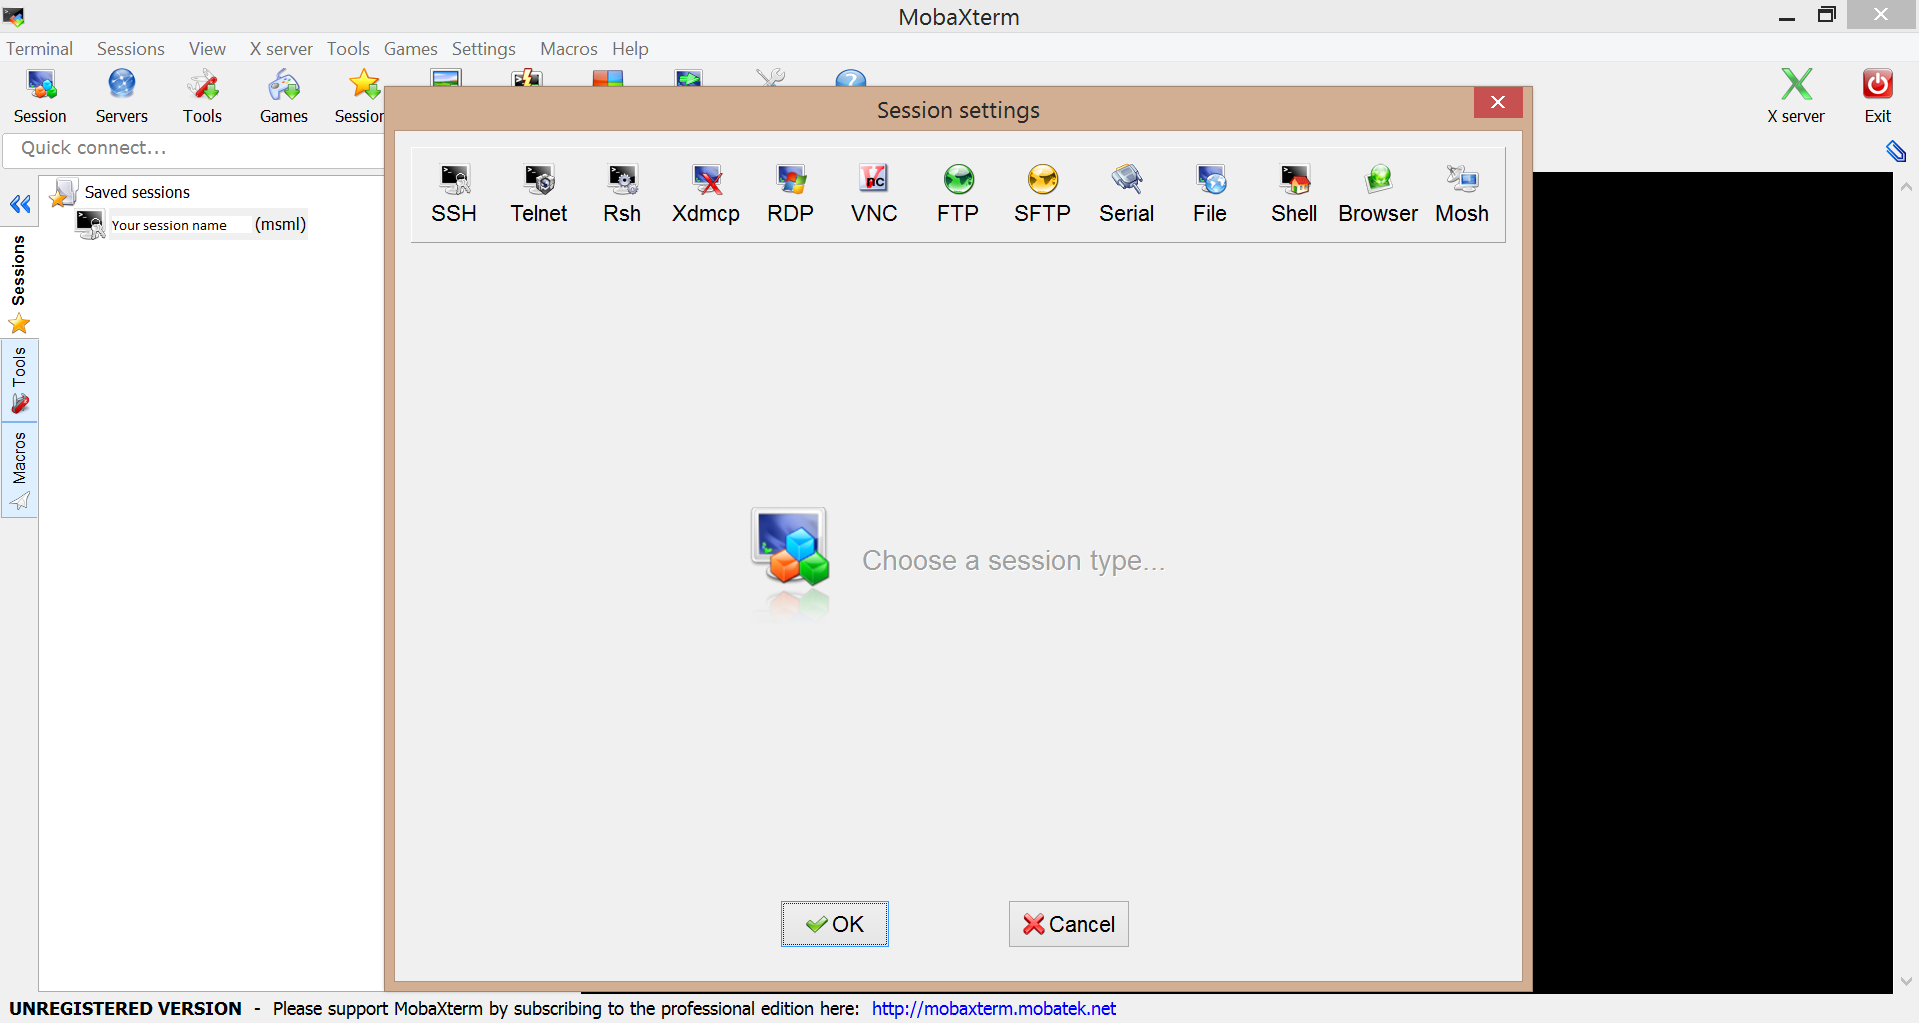
\includegraphics[width=\textwidth]{pictures/MobaXterm_newSession}
    \caption{Screenshot of MobaXterm after starting a new session.}
    \label{mobaXtermNewSession}
\end{figure}

 
\begin{figure}[h]
  	\centering
    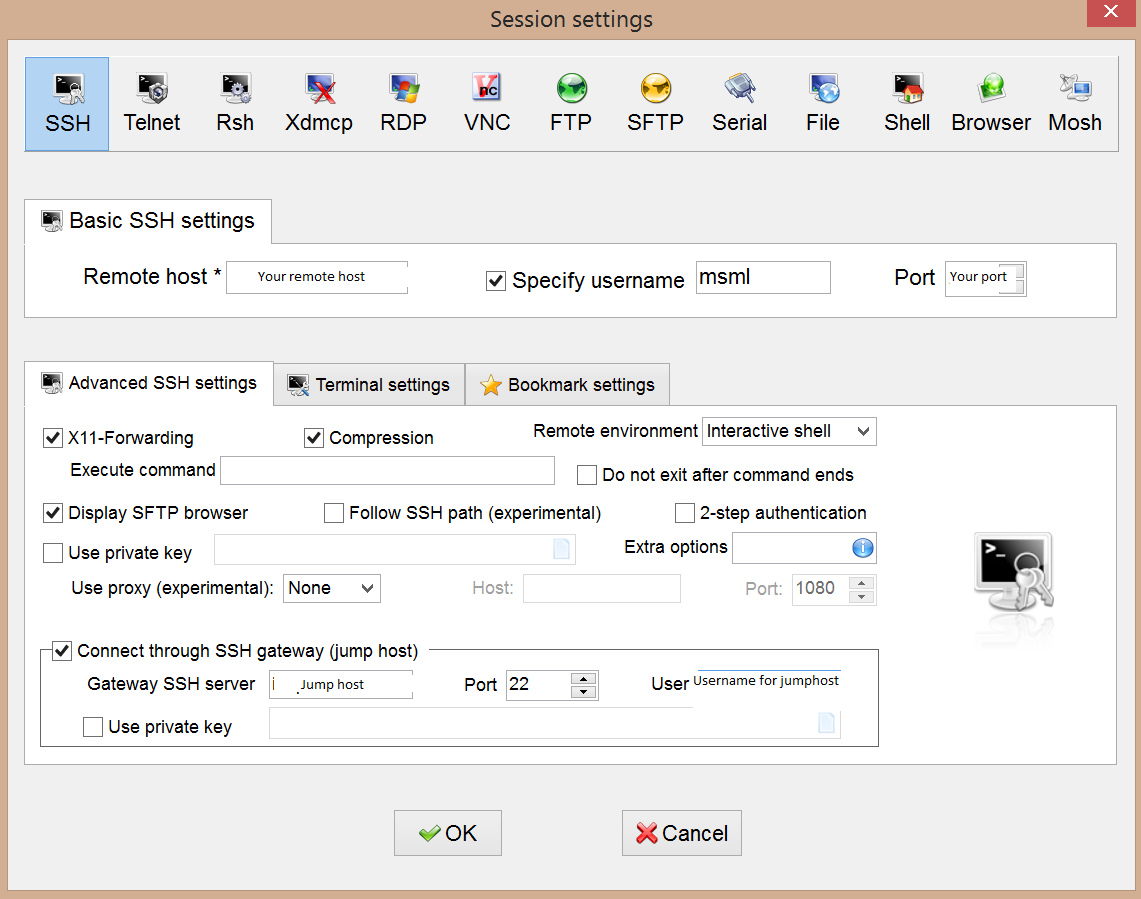
\includegraphics[width=\textwidth]{pictures/MobaXterm_SessionConfig}
    \caption{Screenshot of MobaXterm after starting a new session.}
    \label{mobaXtermSessionConfig}
\end{figure}

 
%\section{Own Installation}
%\label{sec:own-installation}
%
%If you need better OpenGL support or more speed, you should install SOFA and MSML by yourself. This process takes a couple of time for installing several dependencies and  compiling. You should calculate with two or three hours, depending on your system performance.
%
%\subsection{SOFA Installation}
%\label{sec:sofa-installation}
%
%Start by getting the latest SOFA version\footnote{More detail: \url{https://wiki.sofa-framework.org/wiki/Getting_Started}}. 
%
%\begin{lstlisting}[language=sh, breaklines=true]
%git clone --depth 1 git://scm.gforge.inria.fr/sofa/sofa.git
%\end{lstlisting}
%For the compilation you need to install following packages (Ubuntu): 
%\begin{lstlisting}[language=sh, breaklines=true]
%sudo apt-get install cmake cmake-qt-gui cmake-curses-gui ccache \
%build-essential libqt4-dev libglew-dev\
%freeglut3-dev libpng-dev zlib1g-dev\
%python2.7-hdev libxml2-dev libcgal-dev libblas-dev\
%liblapack-dev libsuitesparse-dev \
%libboost-all-dev libassimp-dev 
%\end{lstlisting}
%
%Create a new folder, go into it, and trigger CMake. 
%
%\begin{lstlisting}[language=sh, breaklines=true]
%mkdir sofa-build
%cd sofa-build
%cmake ../sofa
%cmake ../sofa 
%make -j 8
%\end{lstlisting}
%
%\subsection{MSML}
%
%MSML consists of two parts: C++ functionality and a Python core.  
%First, check out the MSML repository:
%
%\begin{lstlisting}[language=sh, breaklines=true]
%git clone --depth 1 https://github.com/CognitionGuidedSurgery/msml.git
%\end{lstlisting}
%
%
%For C++ we need several libraries (Ubuntu):
%
%\begin{lstlisting}[language=sh, breaklines=true]
%sudo apt-get install libtet1.5-dev libcgal-dev libvtk6-dev \
%libxml2-dev  
%libboost-filesystem-dev libboost-python-dev \
%libboost-program-options-dev libboost-graph-dev \
%libboost-iostreams-dev \
%python-vtk6 swig python-pip 
%\end{lstlisting}
%
%The CMake build process takes care about everything else.
%
%\begin{lstlisting}[language=sh, breaklines=true]
  %mkdir msml-build
  %cd msml-build
  %cmake ../msml/operators
  %make -j 8
%\end{lstlisting}
%
%The Python dependencies are installed via pip:
%
%\begin{lstlisting}[language=sh, breaklines=true]
%pip install -r msml/requirements.txt
%\end{lstlisting}
%
%
%
%
%%%% Local Variables:
%%%% mode: latex
%%%% TeX-master: "../SoftTissueSimulationBook"
%%%% End:

\chapter{Tutorial 1: Phenomenological Modeling}  

\section{Pendulum with implicit Euler time integration}

Start the SOFA scene file \emph{Spring\_EulerImplicit.scn} that describes a simple mass-spring system which is discretized using an implicit Euler scheme.

If you are using the pre-built Docker container this can be achieved by executing
\begin{lstlisting}[language=sh, breaklines=true]
$ cd /opt/sofa/bin 
\end{lstlisting}

\begin{lstlisting}[language=sh, breaklines=true]
$ ./runSofa /home/msml/tutorials/Tutorial1/Spring_EulerImplicit.scn
\end{lstlisting}

In order to see the spring-mass model as shown Fig. \ref{PendulumScreenshot}, please click \emph{All} in the tab \emph{View}. To animate a scene click on \emph{animate}. For moving a particle press \emph{shift} and click on the specified particle.

\begin{figure}[h]
  	\centering
    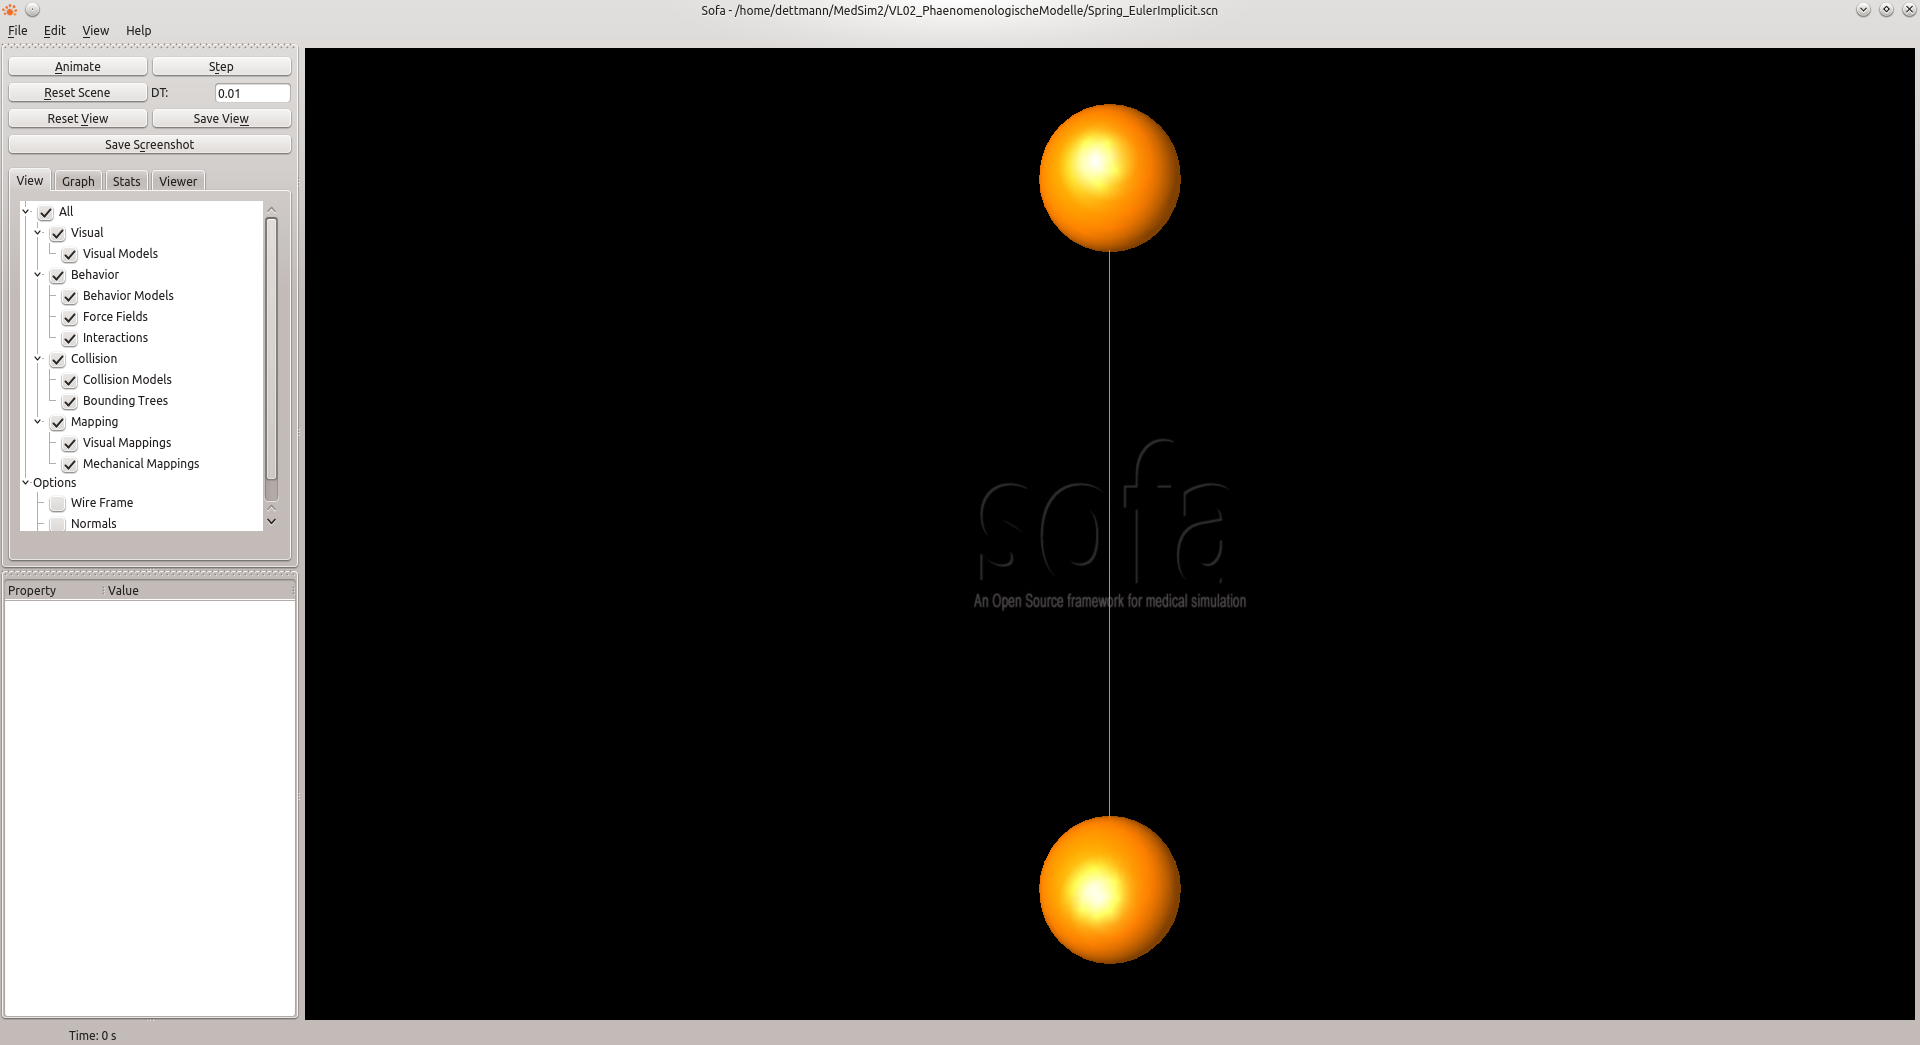
\includegraphics[width=\textwidth]{pictures/sofa_screenshot.png}
    \caption{SOFA framework running a simple pendulum simulation.}
    \label{PendulumScreenshot}
\end{figure}

Parametric studies can be used to get a better understanding of numerical methods. In order to analyze the implicit Euler technique, change the following input parameters
\begin{itemize}
	\item time step size dt in s [0.001, 0.01, 0.1, 1]
	\item stiffness $K_s$ and damping coefficient $K_d$ of the spring (spring='Id1, Id2, $K_s$, $K_d$, L')
\end{itemize}

The parameters can be changed by opening the SOFA scene file (.scn) in a suitable text editor, e.g.
\begin{lstlisting}[language=sh, breaklines=true]
$ geany /home/msml/tutorials/Tutorial1/Spring_EulerImplicit.scn &
\end{lstlisting}

While changing the parameters observe the behavior of the simulation. In particular, try to answer the following questions
\begin{itemize}
	\item How does the parameter effect the stability of the simulation?
	\item Does the frequency or amplitude change?
	\item How does the energy of the system behave over time?
\end{itemize}

\section{Pendulum with explicit Euler time integration}

The pendulum can also be discretized with an explicit Euler time integration scheme (\emph{Spring\_EulerImplicit.scn}). Repeat your analysis on this set-up. In particular, compare the behavior of the explicit and the implicit scheme. 

\chapter{Tutorial 2: Simple Beam Model with MSML}

The medical simulation markup language (MSML) is a flexible XML-based description for the biomechanical modeling workflow and finite-element based biomechanical models.

The example files include several scenarios based on a simple beam model. One scenario describes a linear elastic beam under gravity load. If you are using the pre-built Docker container you can open the scenario with 
\begin{lstlisting}[language=sh, breaklines=true]
$ geany /opt/msml/examples/BeamExample/beamLinearGravity.msml.xml
\end{lstlisting}

In order to simulate the scenario the MSML exec command can be executed from the command line:
\begin{lstlisting}[language=sh, breaklines=true]
$ cd /opt/msml/src
\end{lstlisting}
\begin{lstlisting}[language=sh, breaklines=true]
$ ./msml.py exec -o outputfolderPath /opt/msml/examples/BeamExample/beamLinearGravity.msml.xml
\end{lstlisting}

To get the help information of MSML type the following:
\begin{lstlisting}[language=sh, breaklines=true]
$ ./msml.py -h (or for methods: $ ./msml.py exec -h)
\end{lstlisting}

ParaView can be used to view the results and inspect the meshes:
\begin{lstlisting}[language=sh, breaklines=true]
$ cd /opt/paraview/bin
\end{lstlisting}
\begin{lstlisting}[language=sh, breaklines=true]
$ ./paraview
\end{lstlisting}

After starting ParaView as shown in Fig. \ref{ParaViewScreenshot} you have to load the output file (
before you can press \emph{play} you have to click on \emph{Apply} in the tab \emph{Properties}). The output mesh for each timestep is usually labeled 'dispx.vtu'.

\begin{figure}[h]
  	\centering
    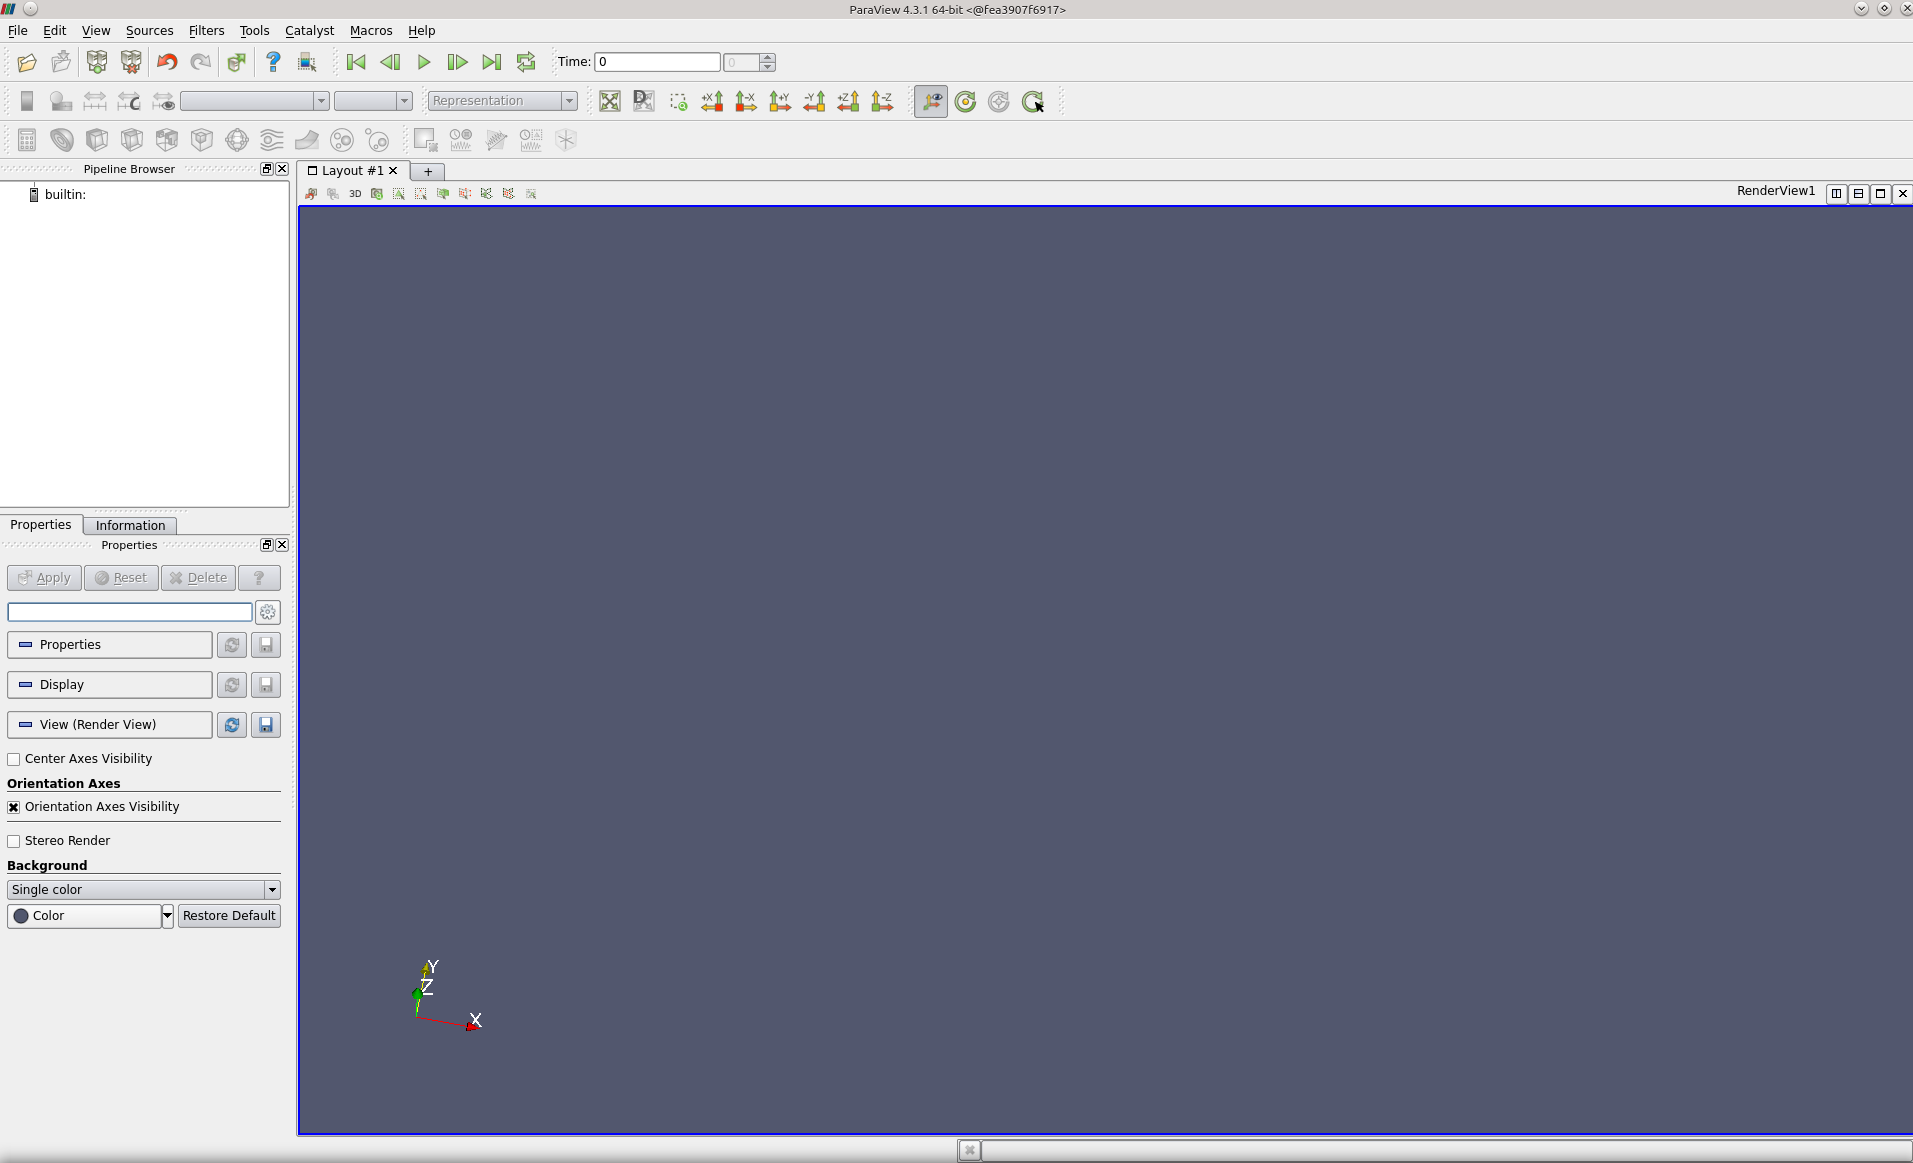
\includegraphics[width=\textwidth]{pictures/start_paraview.png}
    \caption{Start window of ParaView.}
    \label{ParaViewScreenshot}
\end{figure}

The scenario settings (e.g. material parameters, boundary conditions) can be changed by opening the XML-file in a suitable text editor, e.g.
\begin{lstlisting}[language=sh, breaklines=true]
$ geany /opt/msml/examples/BeamExample/beamLinearGravity.msml.xml &
\end{lstlisting}





\section{Using the Python API}

This section describes how to create a running script for MSML in Python.

First open an editor (e.g. geany) and create a new file \emph{myScript.py}.
To run MSML from a python environment we need some imports as described in the following:
\begin{lstlisting}[language=Python]
import os
import sys
sys.path.insert(0, envconf.MSML_ROOT)) #to use msml imports
import msml.api.simulation_runner as api
\end{lstlisting}

Then you have to define the input file and the output directory:
\begin{lstlisting}[language=Python]
msml_infile = os.path.abspath("/opt/msml/examples/LiverExample/liverLinear.msml.xml")
msml_outdir = os.path.abspath("/tmp/MSMLResultsBeam/")
\end{lstlisting}

To start MSML the following code is necessary:
\begin{lstlisting}[language=Python]
myRunner = api.SimulationRunner(msml_infile, "sofa", msml_outdir)
myRunner.run()
\end{lstlisting}

Now your script is complete. Start the script with
\begin{lstlisting}[language=sh, breaklines=true]
$ python myScript.py
\end{lstlisting}
 


\bibliography{bibliography}
\bibliographystyle{alpha} %for english bib
\interlinepenalty=100

\newpage                            
\pagestyle{empty}


\end{document}                          % The required last line


